\documentclass[a4paper,14pt]{extarticle}

\usepackage{cmap}
\usepackage[T2A]{fontenc}
\usepackage[utf8x]{inputenc}
\usepackage[english, russian]{babel}

\usepackage{misccorr} % в заголовках появляется точка, но при ссылке на них ее нет
\usepackage{amssymb,amsfonts,amsmath,amsthm}  
\usepackage{indentfirst}
\usepackage[usenames,dvipsnames]{color} 
\usepackage[unicode,hidelinks]{hyperref}
% \hypersetup{%
%     pdfborder = {0 0 0}
% }

\usepackage{makecell,multirow} 
\usepackage{ulem}
\usepackage{graphicx,wrapfig}
\graphicspath{{img/}}
\usepackage{geometry}
\geometry{left=2cm,right=2cm,top=3cm,bottom=3cm,bindingoffset=0cm,headheight=15pt}
\usepackage{fancyhdr} 
\linespread{1.05} 
\frenchspacing 
\renewcommand{\labelenumii}{\theenumii)} 
\newcommand{\mean}[1]{\langle#1\rangle}
% \usepackage{caption}
%%%%%%%%%%%%%%%%%%%%%%%%%%%%%%%%%%%%%%%%%%%%%%%%%%%%%%%%%%%%%%%%%%%%%%%%%%%%%%%
%%%%%%%%%%%%%%%%%%%%%%%%%%%%%%%%%%%%%%%%%%%%%%%%%%%%%%%%%%%%%%%%%%%%%%%%%%%%%%%

\def\labauthors{Сарафанов Ф.Г., Платонова М.В.}
\def\labgroup{430}
% \def\department{Кафедра электроники и квантовой физики}
\def\labnumber{1}
\def\labtheme{Движение носителей заряда в электрических и магнитных полях}

%%%%%%%%%%%%%%%%%%%%%%%%%%%%%%%%%%%%%%%%%%%%%%%%%%%%%%%%%%%%%%%%%%%%%%%%%%%%%%%
	%применим колонтитул к стилю страницы
\pagestyle{fancy} 
	%очистим "шапку" страницы
\fancyhead{} 
	%слева сверху на четных и справа на нечетных
\fancyhead[L]{\labauthors} 
	%справа сверху на четных и слева на нечетных
\fancyhead[R]{Отчёт по лабораторной работе №\labnumber} 
	%очистим "подвал" страницы
\fancyfoot{} 
	% номер страницы в нижнем колинтуле в центре
\fancyfoot[C]{\thepage} 
\renewcommand{\phi}{\varphi}
%%%%%%%%%%%%%%%%%%%%%%%%%%%%%%%%%%%%%%%%%%%%%%%%%%%%%%%%%%%%%%%%%%%%%%%%%%%%%%%

\usepackage{float}
\usepackage[mode=buildnew]{standalone}
\usepackage{tikz} 
% \usepackage{subcaption}
\usepackage{tikz,csvsimple}
\usetikzlibrary{scopes}
\usetikzlibrary{%
     decorations.pathreplacing,%
     decorations.pathmorphing,%
    patterns,%
    calc,%
    scopes,%
    arrows,%
    % arrows.spaced,%
}
\makeatletter
\newif\if@gather@prefix 
\preto\place@tag@gather{% 
  \if@gather@prefix\iftagsleft@ 
    \kern-\gdisplaywidth@ 
    \rlap{\gather@prefix}% 
    \kern\gdisplaywidth@ 
  \fi\fi 
} 
\appto\place@tag@gather{% 
  \if@gather@prefix\iftagsleft@\else 
    \kern-\displaywidth 
    \rlap{\gather@prefix}% 
    \kern\displaywidth 
  \fi\fi 
  \global\@gather@prefixfalse 
} 
\preto\place@tag{% 
  \if@gather@prefix\iftagsleft@ 
    \kern-\gdisplaywidth@ 
    \rlap{\gather@prefix}% 
    \kern\displaywidth@ 
  \fi\fi 
} 
\appto\place@tag{% 
  \if@gather@prefix\iftagsleft@\else 
    \kern-\displaywidth 
    \rlap{\gather@prefix}% 
    \kern\displaywidth 
  \fi\fi 
  \global\@gather@prefixfalse 
} 
\newcommand*{\beforetext}[1]{% 
  \ifmeasuring@\else
  \gdef\gather@prefix{#1}% 
  \global\@gather@prefixtrue 
  \fi
} 
\makeatother

\usepackage{booktabs}
\usepackage{pgfplots, pgfplotstable}

\usepackage[outline]{contour}
\usepackage{tocloft}
\renewcommand{\cftsecleader}{\cftdotfill{\cftdotsep}} % for parts
% \renewcommand{\cftchapleader}{\cftdotfill{\cftdotsep}} % for chapters
\usepackage{pgfplots,pgfplotstable,booktabs,colortbl}
\pgfplotsset{compat=newest}
\usepackage{physics}
\usepackage{mathtools}
\mathtoolsset{showonlyrefs=true}
\newcommand\Smat{\hat { \mathbf { S } }}

\newcommand*\dotvec[1][1,1]{\crossproducttemp#1\relax}
\def\crossproducttemp#1,#2\relax{{\qty[\vec{#1}\times\vec{#2}\,]}}

\newcommand*\prodvec[1][1,1]{\crossproducttempa#1\relax}
\def\crossproducttempa#1,#2\relax{{\qty[{#1}\times{#2}\,]}}

% \def\E{\mathscr{E}_H}
\def\Rdim{\,\frac{\text{м}^3}{\text{А} \cdot \text{с}}}

\renewcommand{\vec}{\mathbf} % for parts

\begin{document}
\begin{titlepage}
\begin{center}
% \vspace{-3em}
{\small\textsc{Нижегородский государственный университет имени Н.\,И. Лобачевского}}
\vskip 2pt \hrule \vskip 3pt
{\small\textsc{Радиофизический факультет}}

\vfill


{{\large Отчет по лабораторной работе №\labnumber}\vskip 12pt {\LARGE \bfseries Исследование отражательного\\[0.2em] клистрона}}

	
\vspace{2cm}
{\large Работу выполнили студенты \\[-0.25em] 440 группы радиофизического факультата \\[0.5em] {\Large \bfseries \labauthors}}

% \vspace{0.5cm}
% {e-mail: sfg180@yandex.ru}

% \vspace{2cm}

\end{center}

\vfill
	
% \begin{flushright}
% 	{Выполнили студенты 430 группы\\ \labauthor}%\vskip 12pt Принял:\\ Менсов С.\,Н.}
% \end{flushright}
	
% \vfill
	
\begin{center}
	{Нижний Новгород, 10 сентября -- \today}
\end{center}

\end{titlepage}
\tableofcontents
\newpage


\section{Теоретическая часть}

\addcontentsline{toc}{subsection}{Введение}
\subsection*{Введение}

Отражательный клистрон
\footnote{Название <<клистрон>> происходит от греческого слова «клизо», что означает береговой волнорез.}, 
изучению которого посвящена лабораторная работа, предназначен для генерации электромагнитных колебаний СВЧ диапазона. Исторически именно генераторы клистронного типа позволили освоить диапазоны сантиметровых и дециметровых волн, в которых традицион­ные электронные лампы оказались неэффективными [1].

Генерация в клистронах осуществляется за счет преобразования кинетической энергии пучка электронов, ускоренных статическим электрическим полем, в энергию сверхвысокочастотных колебаний. Для получения СВЧ колебаний пучок электронов модулируется по плотности и проводится че­ рез резонатор клистрона, в котором переменный конвекционный ток пучка возбуждает колебания.

Неоднородный электронный поток в приборах клистронного типа созда­ется посредством так называемого динамического способа управления плот­ностью зарядов. При этом способе управления однородный электронный по­ток пропускается через переменное электрическое поле управляющего 
(груп­пирующего) устройства. Переменное поле воздействует на скорости электро­
нов в потоке, периодически ускоряя и замедляя их движение в зависимо­
сти от фазы высокочастотного поля, существующей в момент пролета элек­тронов через управляющее устройство. Возникающее различие в скоростях
электронов приводит к их группировке при последующем движении за пре­
делами управляющего устройства. При этом в определенной точке простран­
ства в определенный момент времени происходит образование электронного
сгустка. Поток приобретает пульсирующий характер, причем электронные
уплотнения и разрежения в данной точке пространства возникают с перио­дичностью, соответствующей частоте управляющего поля
\footnote{При использовании приемов т. н. электростатического управления основной результат управ­
ления состоит в мо дуляции электронного потока по плотности непосредственно в области управ­
ляющего поля [2, 3].}.

Характер процесса группировки электронов, координата и время образования сгустка в клистронах определяются условиями движения вне управляющего промежутка.

В пролетных клистронах группировка происходит при движении электронов по инерции в пространстве, свободном от внешних постоянных или переменных полей; группировка становится возможной за счет того, что «быстрые» электроны догоняют «медленные», вылетевшие из управляюще­го промежутка раньше «быстрых».

В отражательных клистронах электроны, вышедшие из группирующего устройства, движутся в постоянном тормозящем электрическом поле. Значение этого поля таково, что все электроны, вылетевшие из управляющего устройства, возвращаются назад. Группировка в отражательных клистронах происходит благодаря тому, что «быстрые» электроны находятся в пространстве группировки дольше «медленных», и на обратном пути оказывается возможной встреча «быстрых» электронов с медленными, вышедшими из управляющего промежутка позже «быстрых».

Принципиальная схема отражательного клистрона представлена на рис. \ref{fig:1}. Функции управляющего устройства и устройства, накапливающего энергию электромагнитных колебаний в отражательном клистроне, объединены здесь в тороидальном резонаторе.

\begin{figure}[h!]
  \centering
  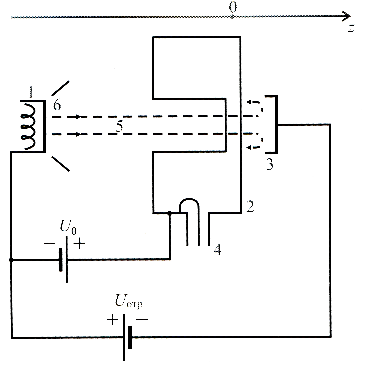
\includegraphics[width=0.4\textwidth]{fig/fig1}
  \caption{Идеализированная принципиальная схема клистрона: 1 — катод, 2 — резонатор, 3 — отражатель, 4 — вывод энергии, 5 — электронный поток, 6 — управляющий электрод}
  \label{fig:1}
\end{figure}

Электронный поток, эмитируемый катодом, ускоряется в промежутке между катодом и резонатором, после чего первый раз попадает в зазор резонатора, образованный двумя прозрачными для потока металлическими сетками. В зазоре происходит модуляция электронного потока по скорости. После выхода из резонатора электроны движутся в тормозящем поле отражающего электрода, возвращаются назад и повторно проходят зазор. При соответствующем выборе потенциалов на электродах клистрона сгусток электронов формируется в сечении зазора резонатора в момент времени, когда высокочастотное поле в зазоре тормозит возвращающиеся электроны, при этом происходит преобразование кинетической энергии электронов в энергию колебаний резонатора. Существование стационарных колебаний в клистроне оказывается возможным при компенсации потерь и резонаторе и нагрузке притоком энергии от модулированного электронного потока.

\subsection{Резонатор клистрона}

Резонатор в клистроне выполняет две функции: служит для модуляции электронного потока по скорости и для преобразования кинетической энергии пучка электронов в энергию электромагнитного ноля. Использовать для выполнении этих функций резонатор, геометрические размеры которого сравнимы с длиной волны основного колебания, возбуждаемого в них, невозможно из-за низкой эффективности взаимодействия электромагнитного поля и пучка электронов, пролетающих через этот резонатор
\footnote{Следует отметить, что существует способ группировки электронного потока по плотности, при котором модулируемый поток проводится через область, в которой фаза управляющего поля успевает многократно измениться за время пролета электрона. При использовании этого способа скорости электронов на выходе из управляющего поля окатываются практически одинаковыми, а электронный поток промодулированным по плотности [3].}. Действительно. если средняя скорость электронов $v$ значительно меньше скорости света $с$, то время их пролета $t = a/v$ через резонатор, имеющий форму ку­ ба со стороной а, намного превосходит период колебания поля $T =\sqrt{2}a/c$. Электрон при движении через такой резонатор то ускоряется, то тормозится, поэтому обмен энергией между ним и полем незначителен. Время пролета можно уменьшить, взяв вместо куба призму с достаточно малой высотой:
при неизменной низшей частоте колебаний время пролета электрона через резонатор уменьшается. Однако сокращение объема резонатора приводит к
уменьшению его добротности. Использование в генераторе низкодобротной колебательной системы не позволяет производить эффективное преобразование кинетической энергии электронов в энергию электромагнитных колебаний и не обеспечивает стабильности частоты генератора.

Для увеличения объема резонатора и его добротности необходимо, оставляя длину пролетного промежутка малой, создавать дополнительные резервуары энергии. Именно такой резонатор используется в отражательном клистроне.

Схема резонатора представлена на рис. \ref{fig:2}. Геометрические размеры резонатора удовлетворяют неравенствам $a,b \ll \lambda /4,l \ll \lambda /4,d \ll l$, где $\lambda$ — длина волны, соответствующая частоте основной моды резонатора. По­скольку размеры резонатора много меньше длины волны на частоте основ­
ного колебания, резонатор можно рассматривать как колебательный контур с сосредоточенными параметрами.

При этом в резонаторе можно выделить емкостной объем, заключенный между сетками резонатора, и индуктивный объем, т. е. собственно тороидальную часть.

\begin{figure}[H]
  \centering
  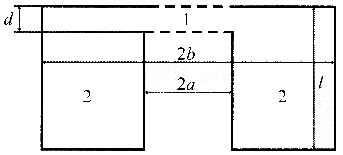
\includegraphics[width=0.5\textwidth]{fig/fig2}
  \caption{Поперечное сечение тороидального резонатора: 1 — емкостной объем резонатора, 2 — индуктивный объем резонатора}
  \label{fig:2}
\end{figure}

При наличии потерь энергии поля в резонаторе, возникающих из-за конечной проводимости стенок и отвода мощности в нагрузку, свободные колебания резонатора являются затухающими, при этом в рамках метода комплексных амплитуд удобно вводить комплексную частоту $\omega = w^{\prime}+i\omega ^{\prime \prime}$. Ве­
личина $\omega ^{ \prime \prime }$ может быть выражена через добротность резонатора, которая, как правило, измеряется экспериментально.

В клистронах применяются резонаторы, допускающие механическую перестройку резонансной частоты. Наиболее распространены два способа перестройки: индуктивный и емкостной. Индуктивная перестройка осуществляется введением в область магнитного поля металлических поршней, кото­рые, уменьшая занятый полем объем, уменьшают индуктивность резонатора и тем самым повышают его резонансную частоту. Емкостная перестройка может быть осуществлена путем деформации гибкой мембраны. Сближение сеток резонатора, обеспечиваемое прогибом мембраны, ведет к увеличению емкости зазора и уменьшению резонансной частоты. Механические способы перестройки обеспечивают отстройку от основной частоты на 20-25\%.

\subsection{Модуляция скорости электронов в пучке}

Рассмотрим процесс модуляции электронного потока по скорости. В установившемся режиме колебания в резонаторе близки к гармоническим, поле в зазоре имеет вид 
$E = E _ { z } = E _ { m } \text { sin } \omega t$, 
где $E _ { m } = \frac { U _ { m } } { d }$, $U _ { m }$ амплитуда напряжения на зазоре,$E _ { z }$ проекция электрического ноля на ось $z$,
$d$ - ширина зазора, $\omega$ частота стационарных колебаний. Найдем приращение энергии электрона, прошедшего через зазор. Кинетическая энергия,
приобретаемая одиночным электроном при прохождении пути $\dd z$ внутри за­зора, равна работе силы электрического поля: 
$\dd W = - e \frac { U _ { m } } { d } \sin \omega t \dd z$, 
где $e$ - модуль заряда электрона (знак заряда учтен в явном виде)
\footnote{Если напряжение (потенциал второй сетки относительно первой) $U = -U_m \sin \omega t$ положительно, оно ускоряет электрон, движущийся в положительном направлении оси z.}. 
Электрон, прошедший расстояние между катодом и резонатором, имеет кинетическую энергию 
$\frac { m v _ { 0 } ^ { 2 } } { 2 } = e U _ { 0 }$ , где $U_0 > 0$-- потенциал резонатора относительно ка­тода, $v_0$ — скорость электрона, $m$ — его масса. Отсюда при условии $v _ { 0 } \ll c$ имеем
\footnote{Пренебрежение релятивистскими поправками возможно до значений $U_0$ порядка нескольких
десятков киловольт.} 
$v _ { 0 } = \sqrt { \frac { 2 e U _ { 0 } } { m } }$

При выполнении условия 
$\frac { U _ { m } } { U _ { 0 } } \ll 1$ возмущения скорости $v_0$ под воздействием высокочастотного поля незначительны. Поэтому если $t_0$ — время про­
хождения электроном центра зазора, то время его нахождения в точке с координатой $z$ есть $t = t _ { 0 } + \frac { z } { v _ { 0 } }$. Полное приращение энергии имеет вид

\begin{equation}
   { \Delta W = \int\limits _ { - d / 2 }^{{ + d / 2 }} \frac { - e U _ { m } } { d } \sin \left( \omega t _ { 0 } + \frac { \omega z } { v _ { 0 } } \right) d z = } \\ 
   { - e U _ { m } \sin \omega t _ { 0 } \frac { \sin \left( \theta _ { 3 } / 2 \right) } { \theta_ { 3 } / 2 } = - e M U _ { m } \sin \omega t _ { 0 }, } 
\end{equation}

где $\theta _ { 3 } = \frac { \omega d } { t _ { 0 } }$ - невозмущенный угол пролета электрона через модулирующий зазор, $M = \frac { \sin \left( \theta _ { 3 } / 2 \right) } { \theta _ { 3 } / 2 }$ - коэффициент взаимодействия электронного потока с полем зазора. Полная кинетическая энергия электрона, вошедшего в зазор с начальной скоростью на выходе из него может быть представлена в виде:
\begin{equation}
  W = \frac { m v ^ { 2 } } { 2 } = \frac { m v_0 ^ { 2 } } { 2 } + \Delta W = e U _ { 0 } + \Delta W.
\end{equation}
Таким образом, скорость электрона на выходе из зазора оказывается равной
\begin{equation}
  v = \sqrt { \frac { 2 e } { m } U _ { 0 } } \left( 1 - \frac { M U _ { m } } { U _ { 0 } } \sin \omega t _ { 0 } \right) ^ { 1 / 2 }.
\end{equation}
При выполнении условия $\frac { U _ { m } } { U _ { 0 } } \ll 1$ можно разложить выражение для $v$ в ряд Тейлора и ограничиться двумя первыми членами ряда:
\begin{equation}
  v = \sqrt { \frac { 2 e } { m } U _ { 0 } } \left( 1 - \frac { 1 } { 2 } \frac { M U _ { m } } { U _ { 0 } } \sin \omega t _ { 0 } + \ldots \right) \approx v _ { 0 } - v _ { 1 } \sin \omega t _ { 0 },
\end{equation} где $v _ { 1 } = \frac { M U _ { m } } { 2 U _ { 0 } } v _ { 0 }$
Из полученного выражения видно, что скорость электро­на на выходе из зазора определяется фазой поля, существовавшей в момент прохождения им центра зазора. Наибольшая амплитуда скоростной модуляции $v_1$ достигается при стремлении коэффициента взаимодействия $M$ к единице, что выполняется при стремлении $\theta_3$ к нулю.

\subsection{Модуляция электронного пучка по плотности}

В пространстве между резонатором и отражателем электроны двигаются в статическом тормозящем поле. Уравнение движения имеет вид 
$mz''- e \frac { U _ { 0 } - U _ { \text{отр} } } { L }$ где $U_{\text{отр}} < 0$ — напряжение на отражателе, $L$ — расстояние между резонатором и отражателем. Интегрируя первый раз уравнение движения и учитывая выражение для скорости $v$ при выходе из зазора, имеем
\begin{equation}
  z ^ { \prime } = v - \frac { e } { m } \frac { U _ { 0 } - U _ { \text { отр } } } { L } \left( t - t ^ { \prime } \right)
\end{equation}
где $t'$ — момент выхода электрона из зазора. Через t в дальнейшем будем обозначать момент, когда тот же электрон возвращается в плоскость второй сетки. Повторное интегрирование уравнения (5) дает
\begin{equation}
  z = v \left( t - t ^ { \prime } \right) - \frac { e } { m } \frac { U _ { 0 } - U _ { \text { отр } } } { L } \frac { \left( t - t ^ { \prime } \right) ^ { 2 } } { 2 } + \frac { d } { 2 }
\end{equation}

Время пролета электрона в пространстве группировки можно найти из условия $z = d / 2$ при $t=t''$, откуда следует, что 
$t ^ { \prime \prime } - t ^ { \prime } = 0$ и 
$\frac { e } { m } \frac { U _ { 0 } - U _ { \text { отр } } } { L }\cdot \frac { \left( t ^ { \prime \prime } - t ^ { \prime } \right) } { 2 v } = 1$
Первое решение $(t' = t'' )$ соответствует моменту вылета электрона из зазора, второе дает время его пролета в тормозящем поле:
\begin{equation}
  t ^ { \prime \prime } - t ^ { \prime } = \frac { 2 m } { e } \frac { v L } { L _ { 0 } - U _ { \text { отр } } }
\end{equation}

При выполнении условия $U_{ m } / U _{ 0 } \ll 1$ время пролета в зазоре определяется скоростью $v_0$, поэтому связь времени вылета электрона из зазора со временем его нахождения в центре зазора можно приближенно записать в виде
$t'' = t _ { 0 } + d / \left( 2 v _ { 0 } \right)$. Таким образом, подставляя выражение для скорости (4) в (7), получим
\begin{equation}
  t ^ { \prime \prime } = t ^ { \prime } + \frac { 2 m L } { e \left( U _ { 0 } - U _ { \text { отр } } \right) } \left( v _ { 0 } - \frac { M U _ { m } } { 2 U _ { 0 } } v _ { 0 } \sin \left( \omega t ^ { \prime } - \frac { \omega d } { 2 v _ { 0 } } \right) \right)
\end{equation}

Из найденного выражения видно, что время пролета электронов в пространстве группировки зависит от фазы высокочастотного напряжения, существующего в момент пролета электроном середины зазора, и от амплитуды этого напряжения.

На рис.\ref{fig:3} представлены примеры пространственно-временных диаграмм(зависимостей координат электронов от времени) для таких значений потенциалов на резонаторе и отражателе, при которых электроны, вышедшие из резонатора в различные моменты времени, возвращаются в него одновремен­но, образуя сгусток. Сверхвысокочастотное поле в резонаторе в рассматриваемых в случаях в момент времени пролета сгустка максимально и является для него тормозящим. Уменьшение кинетической энергии электронов при этом приводит к возрастанию энергии СВЧ поля. Разумеется, при других значениях потенциалов на электродах клистрона сгусток может сформироваться и вне зазора резонатора, при этом эффективная передача энергии от пучка полю становится невозможной.

Домножим соотношение (8) на ы и введем следующие величины:
\begin{equation}
  \theta _ { \text{г} } = \frac { 2 m } { e } \frac { v _ { 0 } \omega L } { U _ { 0 } - U _ { \text{ oтр } } }
\end{equation} — угол пролета электрона в пространстве группировки,
\begin{equation}
  X = \theta _ { \text{г} } \frac{M U _ { m } } { 2 U _ { 0 } }
\end{equation} — параметр группировки. В результате получим выражение, связывающее время возвращения электрона в плоскость второй сетки $(t'' )$ со временем выхода электрона из зазора $(t')$:
\begin{equation}
  \omega t ^ { \prime \prime } = \omega t ^ { \prime } + \theta _ { r } - X \sin \left( \omega t ^ { \prime } - \frac { \theta _ { 3 } } { 2 } \right)
\end{equation}
Соотношение (11) является исходным для нахождения конвекционного тока пучка электронов.

\begin{figure}[h!]
  \centering
  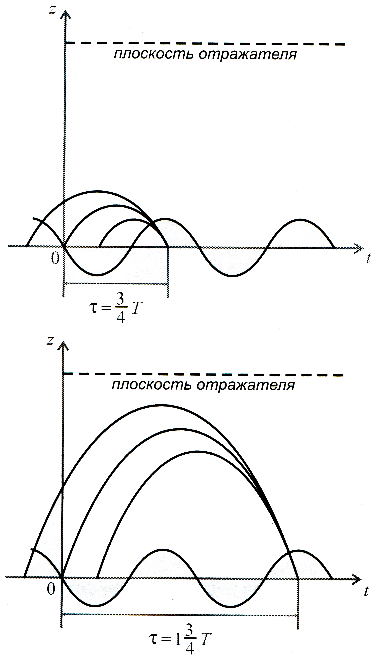
\includegraphics[width=0.5\textwidth]{fig/fig3}
  \caption{Пространственно-временные диаграммы движения электронов при двух значениях оптимального времени пролета $\tau$ в пространстве группировки ($z=0$ координата, соответствующая середине зазора)}
  \label{fig:3}
\end{figure}

\subsection{Возбуждение резонатора клистрона током пучка}
Сгруппированный электронный пучок формирует ток $I$, возбуждающий колебания в резонаторе. При этом условие возбуждения клистрона принимает следующий вид:
\begin{equation}
  \pi + 2 \pi n < \left( \theta _ { 3 } + \theta _ { \text{г} } \right) < 2 \pi ( n + 1 )
\end{equation}где $n=1,2,3,\dots $.

Указанные интервалы углов пролета, при которых возможна генерация, носят название зон генерации клистрона. В центре зон генерации, т. е. при
$\theta _ { \text{г} } + \theta _ { \text{з} } = 2 \pi ( n + 3 / 4 )$ амплитуда максимальна, а на краях равна нулю. Угол пролета в пространстве группировки $\theta _ { \text{г} }$ можно варьировать, изменяя ли­бо напряжение на резонаторе, либо напряжение на отражателе (см. (9)).
Пространственно-временные диаграммы, соответствующие двум оптималь­ным углам пролета, представлены на рис.\ref{fig:3}.

Одной из важных характеристик клистрона является пусковой ток — значение тока $I_0$, при котором клистрон возбуждается:

\begin{equation}
  I _ { 0 \, \text { пуск } } = - \frac { 2 U _ { 0 } G } { M ^ { 2 } 
  \theta _ { \text{ г } } \sin \left( \theta _ { \text{з} } + \theta _ { \text{ г } } \right) }
\end{equation} где G — действительная часть проводимости резонатора.

Как видаю из соотношения (13), пусковой ток клистрона тем меньше, чем меньше величина G. С ростом номера зоны самовозбуждение клистрона облегчается. Ток, требующийся для самовозбуждения клистрона, тем меньше, чем ниже ускоряющее напряжение $U_0$. Легче всего клистрон возбуждается в центрах зон. Напротив, на их краях 
$\sin \left( \theta _ { \text{з} } + \theta _ { \text{г} } \right) \rightarrow 0$ и 
$I _ { 0\, \text { пуск } } \rightarrow \infty$.

\section{Экспериментальная часть}

Исследуемый клистрон предназначен для работы в десятисантиметровом диапазоне.

На рис. \ref{fig:4} показана схема включения клистрона. С блока питания (выпрямители I, II, III) напряжение подается на отражатель, резонатор и управляющий электрод. Контроль величин напряжений на электродах клистрона осуществляется по вольтметру, последовательно подключаемому с помощью
переключателя П1 к любому из электродов. К отражателю клистрона с по­мощью переключателя П2 может подключаться генератор пилообразного
напряжения; СВЧ колебания, генерируемые отражательным клистроном, с помощью петли связи через ответвитель подводятся к кристаллическому
детектору и волномеру ВМТ-10. В цепи детектора стоит микроамперметр, показания которого пропорциональны уровню выходной мощности клистрона
\footnote{При наблюдении зон генерации клистрона на экране осциллографа переключатель П2 ставится  в положение <<модуляция>> (<<Вкл>>), П3--в положение <<Выкл>>(<<Осциллограф>>)}.
\begin{figure}[H]
  \centering
  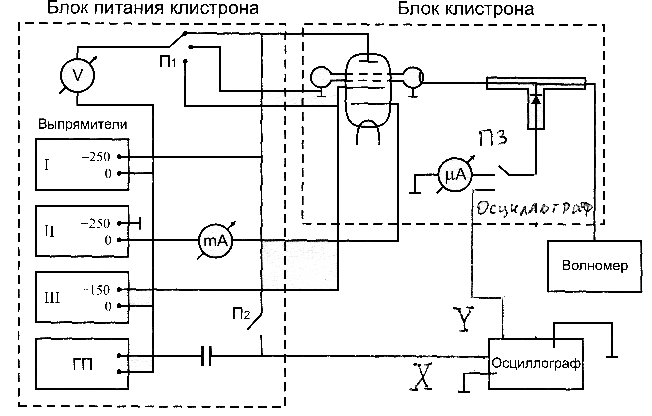
\includegraphics[width=\textwidth]{fig/fig4}
  \caption{ Блок-схема включения клистрона}
  \label{fig:4}
\end{figure}

\subsection{Задания}
\begin{enumerate}
  \item  Включить установку и выставить рабочий режим клистрона, подо­
  брав подходящие значения напряжения на резонаторе (в интервале от 0 до
  -250 В), ускоряющем электроде (от 0 до + 150 В) и отражающем электроде
  (от 0 до —250 В).
  \item  Визуально исследовать режим генерации клистрона на экране осциллографа. Для этого подать на отражатель пилообразное напряжение, поста­
  вив переключатель П2 в положение «модуляция»: На вход Y осциллографа
  подается напряжение с детектора, а на вход X в качестве развертки — пилообразное напряжение с модулятора.
    \begin{enumerate}
      \item Используя кальку, зарисовать зоны генерации клистрона и пронумеровать их. Выяснить, как меняются зоны генерации в зависимости от потенци­
      алов электродов клистрона. Выбрать оптимальный режим работы клистрона (найти значения напряжения на электродах, при которых реализуется
      \item Уменьшая амплитуду пилообразного напряжения на отражателе клистрона, получить на экране только одну зону генерации. Определить с  по­мощью волномера ширину частотной перестройки клистрона. Для этого, из­меняя настройку волномера, проследить на экране осциллографа движение
      метки по зоне генерации. Зафиксировав показания волномера в крайних точках зоны, определить ширину частотной перестройки клистрона вдоль
      зоны генерации.
    \end{enumerate}
  
  При выполнении остальных заданий переключатель П2 должен быть в положении «выкл», при этом должен быть выключен и осциллограф.

  \item Снять зависимости тока в цепи детектора (ток пропорционален мощ­
  ности колебаний) от: 
    \begin{enumerate}
      \item напряжения на отражателе (при нескольких фиксированных напряжениях на резонаторе),
      \item напряжения на резонаторе (при нескольких фиксированных напряжениях на отражателе).
    \end{enumerate} 
  Экспериментальные данные представить в виде графиков.
  
  Рекомендуется снятие характеристик в этом задании совмещать с измерением частотных зависимостей (см. задание 4).

  \item Измерить при помощи волномера длину волны колебаний, генерируемых клистроном, и проследить, как она меняется вдоль каждой зоны. Для
  этого снять зависимости частоты от:
    \begin{enumerate}
      \item  напряжения на отражателе (при фиксированном напряжении на резонаторе) ,
      \item  напряжения на резонаторе (при фиксированном напряжении на отражателе).
    \end{enumerate}
  
  Экспериментальные данные представить в виде графиков.

  \item  Снять зависимость тока в цепи детектора от тока пучка для различных зон генерации клистрона. Потенциал отражателя для каждой зоны устанавливается по максимальной интенсивности колебаний (т.е. в центре зоны). Экспериментальные данные представить в виде графиков. На основании измерений определить пусковой ток клистрона для каждой зоны. Регулировку  тока пучка осуществлять изменением величины потенциала на управляющем электроде.

  \item  Объяснить полученные экспериментальные данные.

\end{enumerate}
\newpage
\subsection{Задание 2}
Значения напряжения на электродах, при которых наблюдаются три зоны генерации клистрона:
\begin{itemize}
  \item $U_{\text{рез}}=96$ В
  \item $U_{\text{уск}}=126$ В
  \item $U_{\text{отр}}=42$ В
\end{itemize}
\begin{figure}[h!]
  \centering
  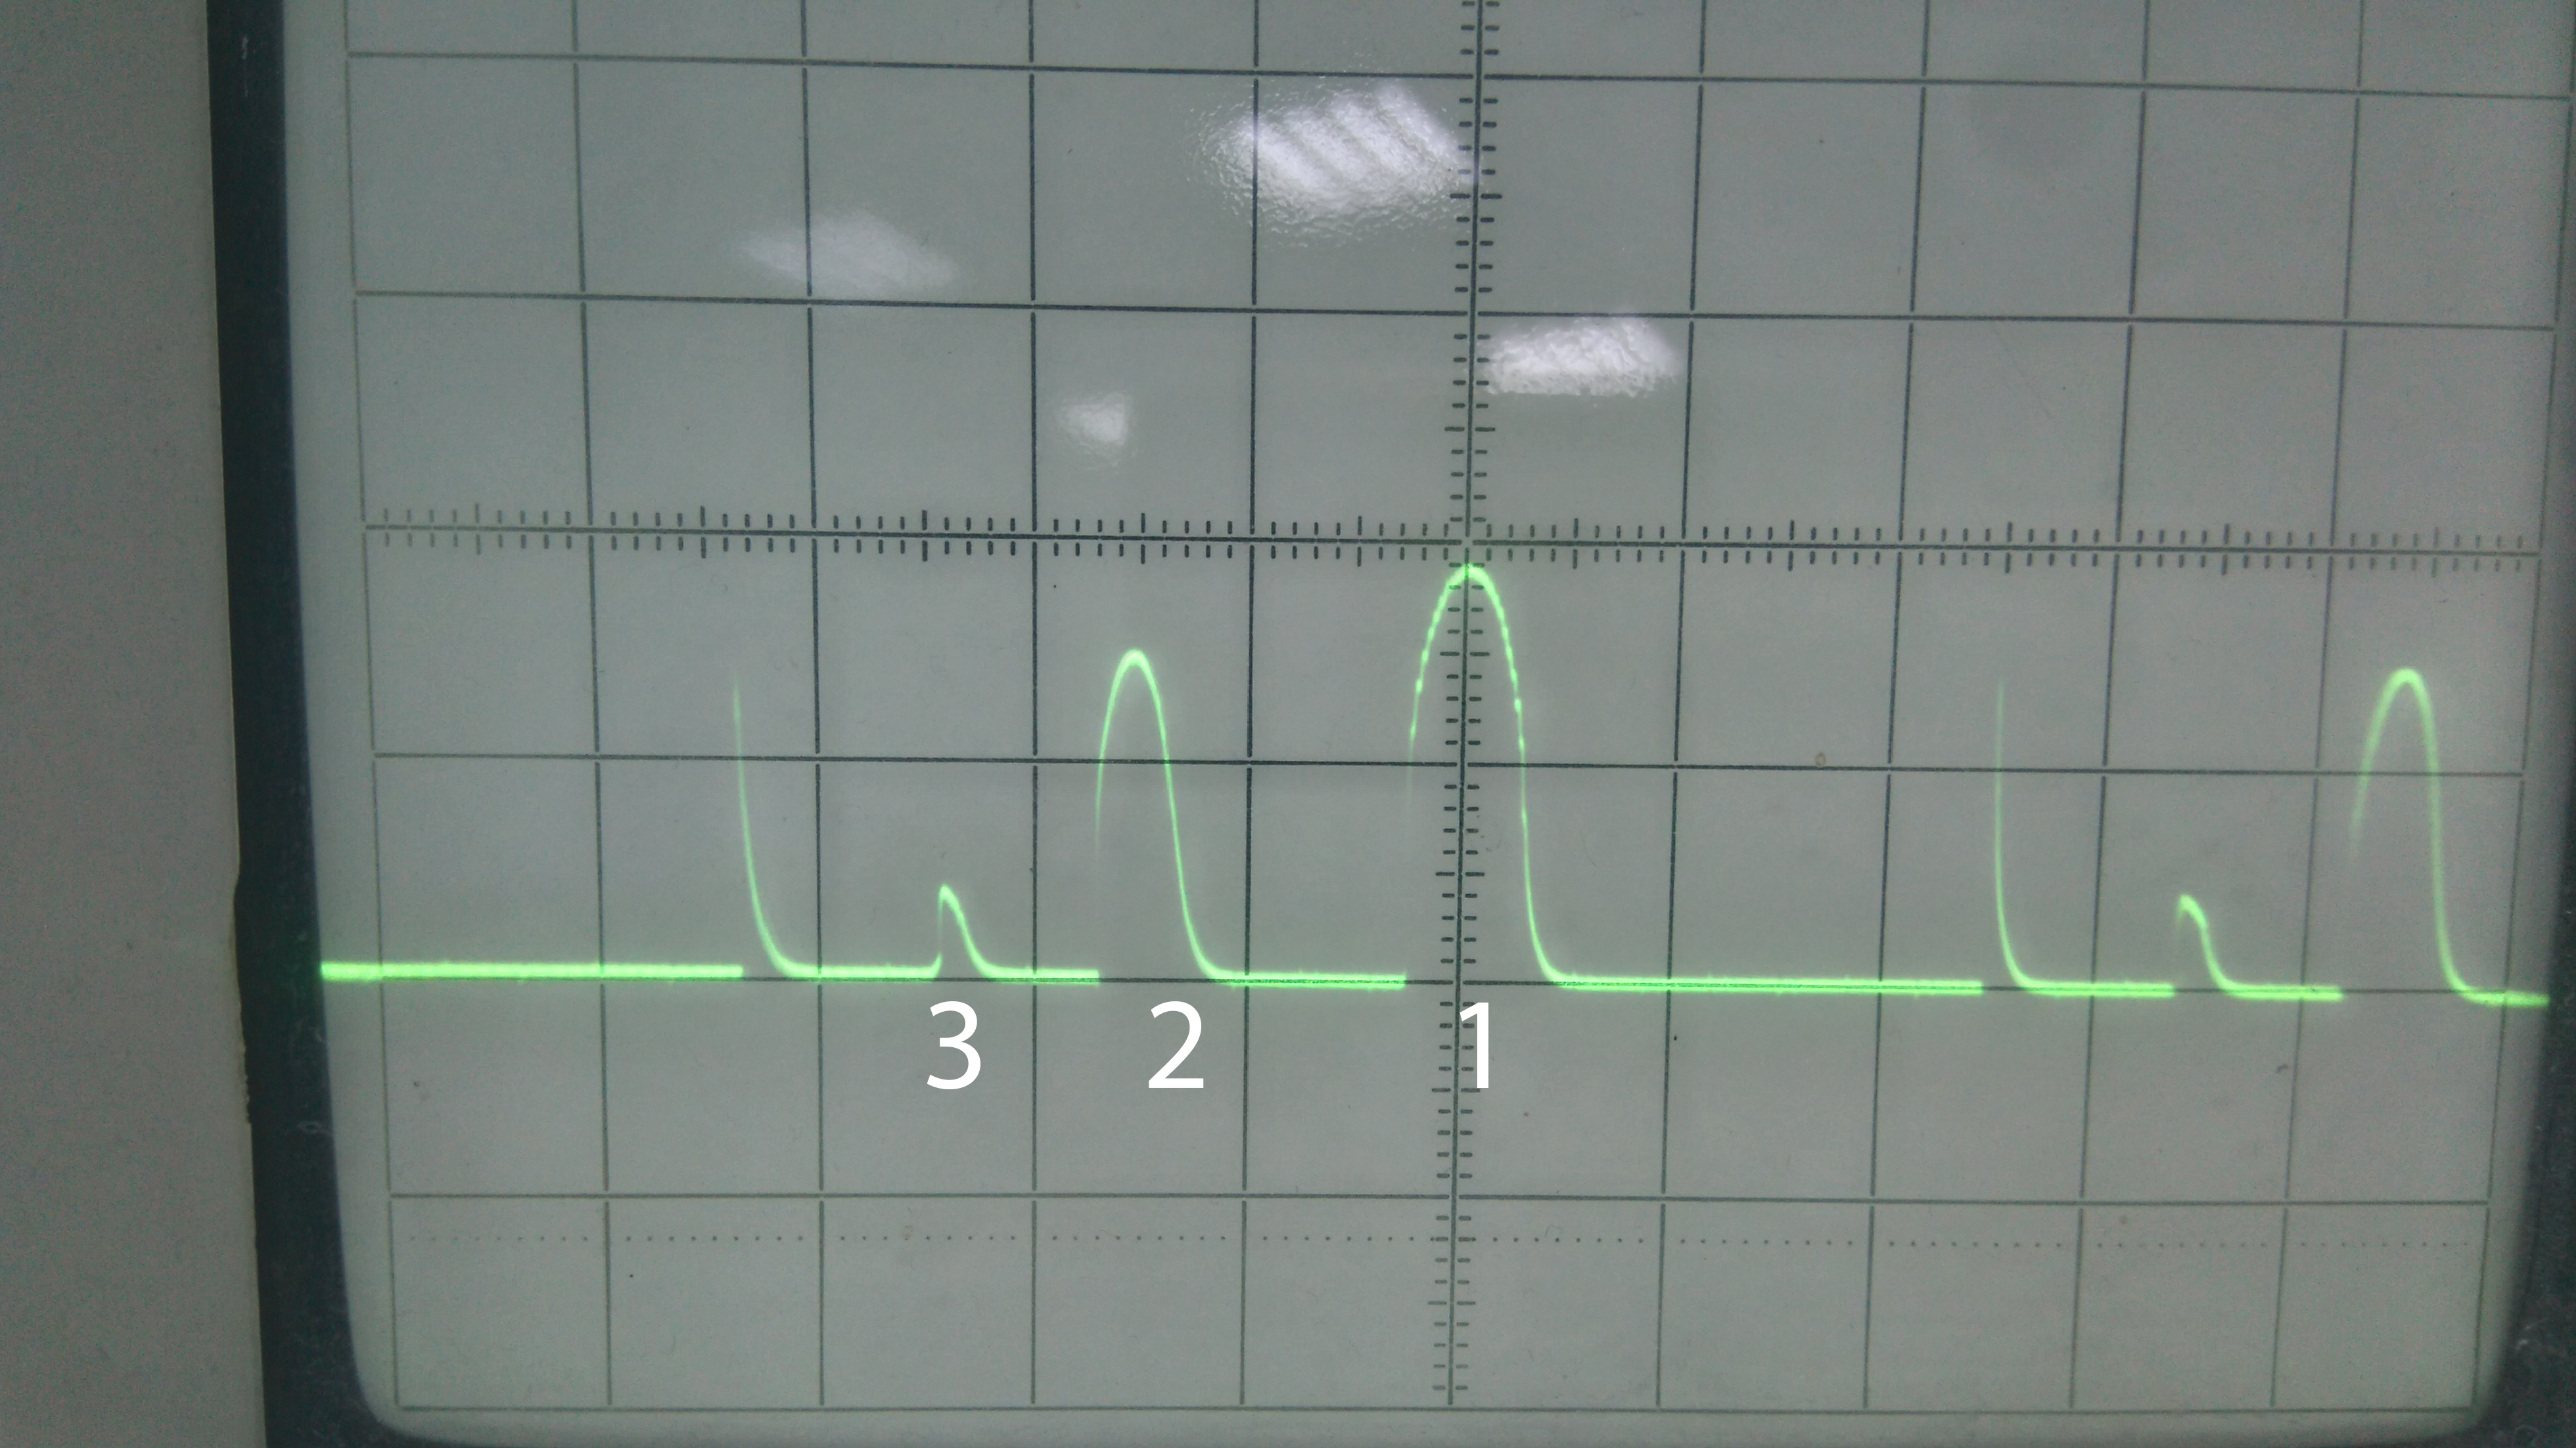
\includegraphics[width=\linewidth]{img/img1}
  \caption{Характерный вид зон генерации клистрона на осциллографе}
  \label{fig:img1}
\end{figure}
\newpage
\begin{figure}[h]
  \begin{minipage}[h]{0.45\linewidth}
    \centering
    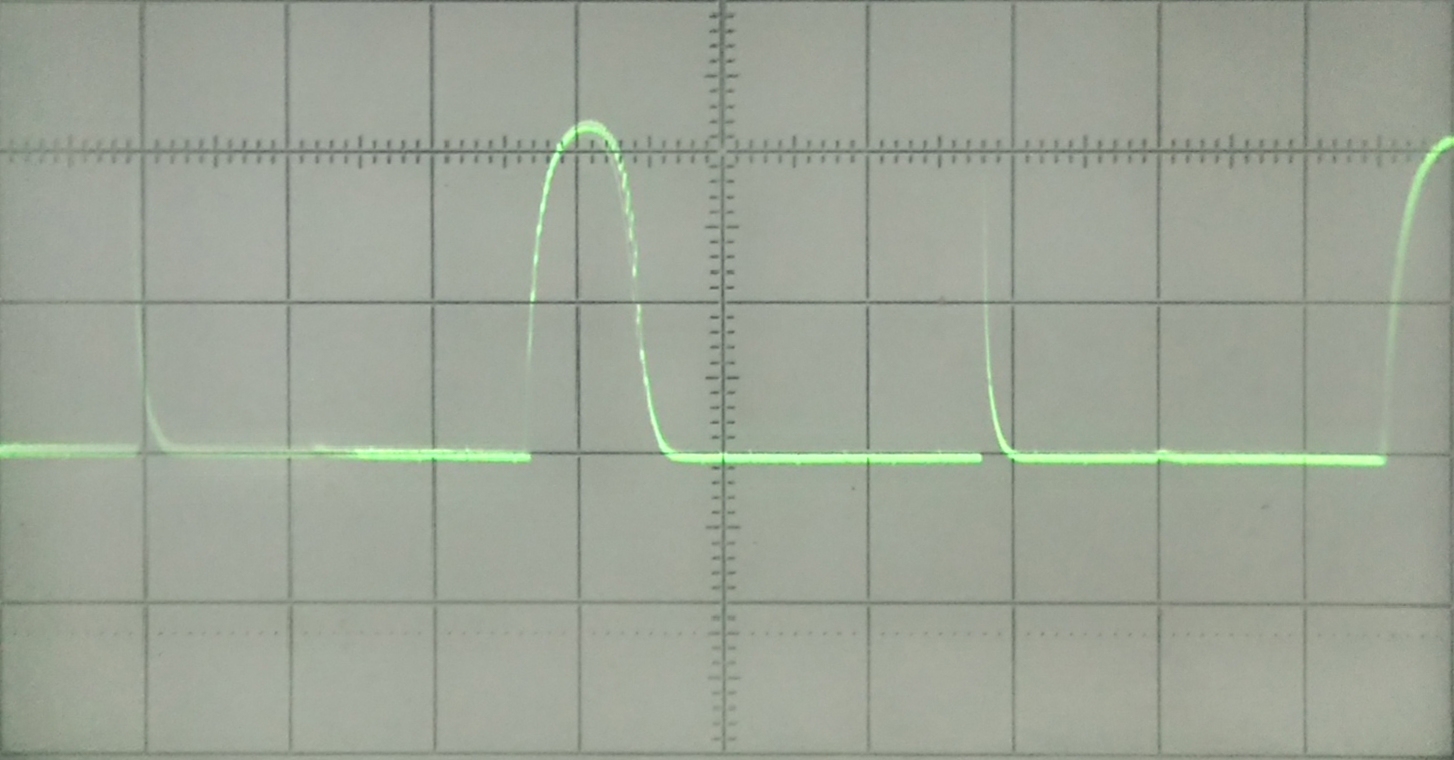
\includegraphics[width=\textwidth]{img/img2}
    \caption{$U_{\text{уск}}=159$ В}
    \label{fig:img2}
  \end{minipage}
  \hfill
  \begin{minipage}[h]{0.45\linewidth}
    \centering
    {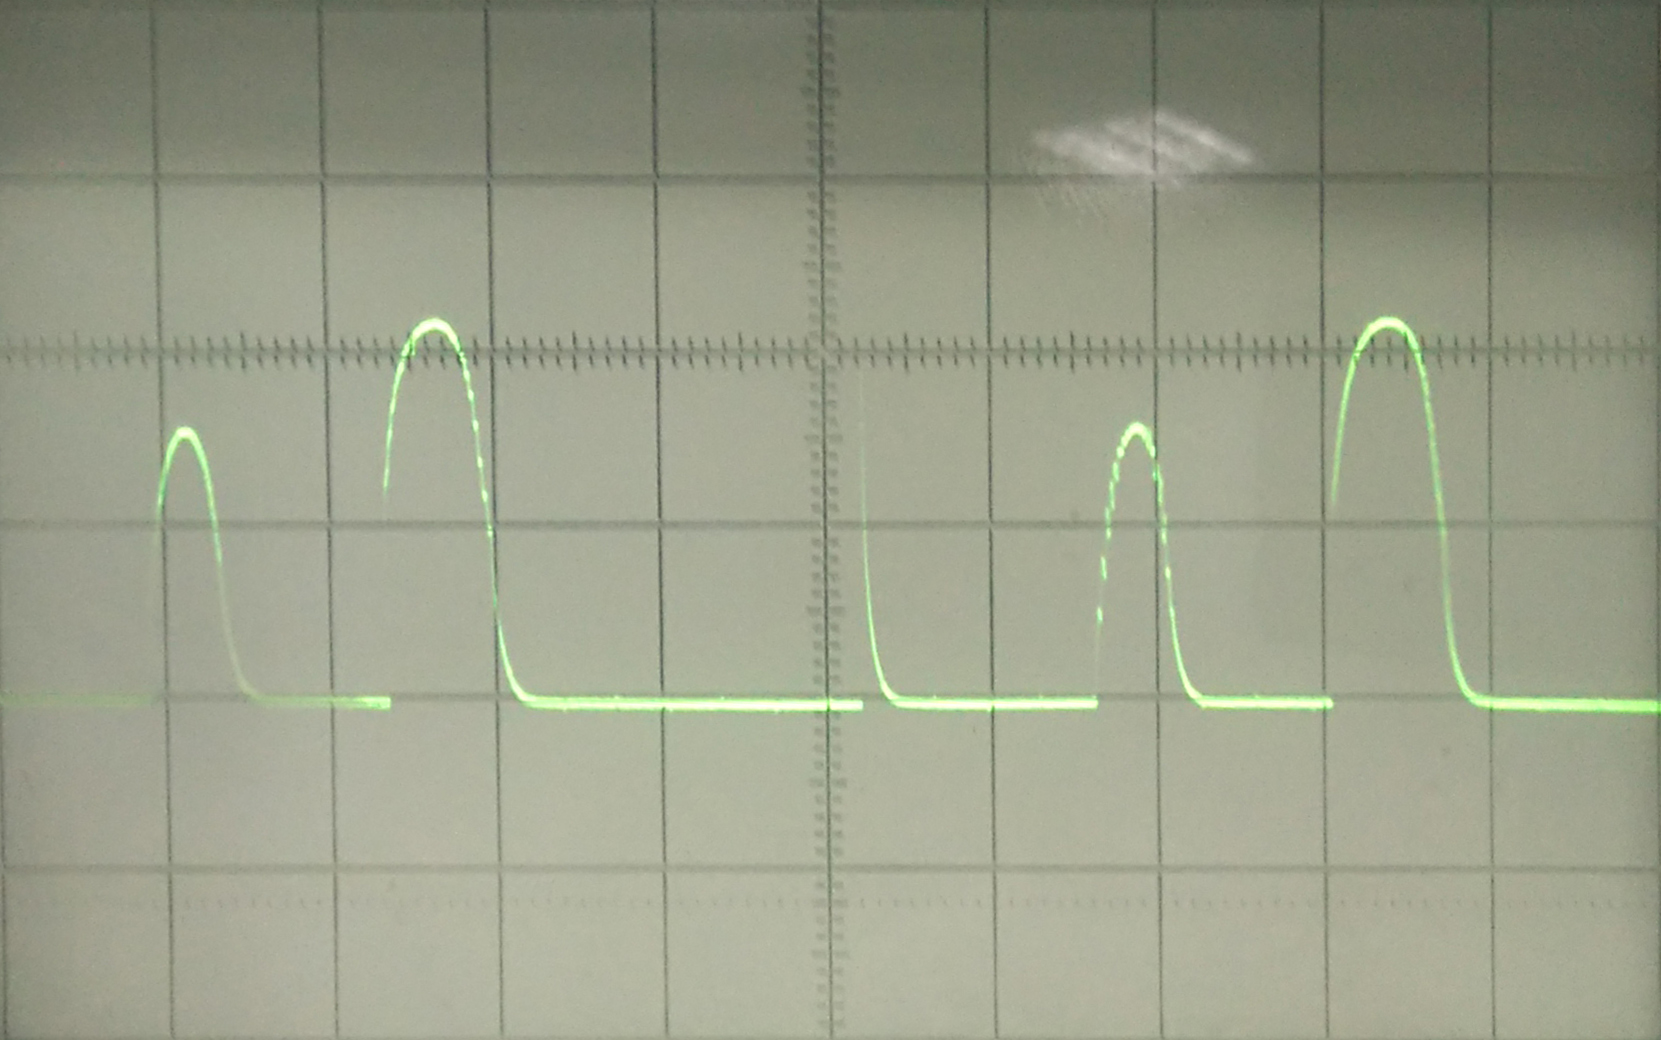
\includegraphics[width=\textwidth]{img/img3}}
    \caption{$U_{\text{уск}}=152$ В}
    \label{fig:img3}
  \end{minipage}
  \vfill
  \vspace{1em}
  \begin{minipage}[h]{0.45\linewidth}
    \centering
    {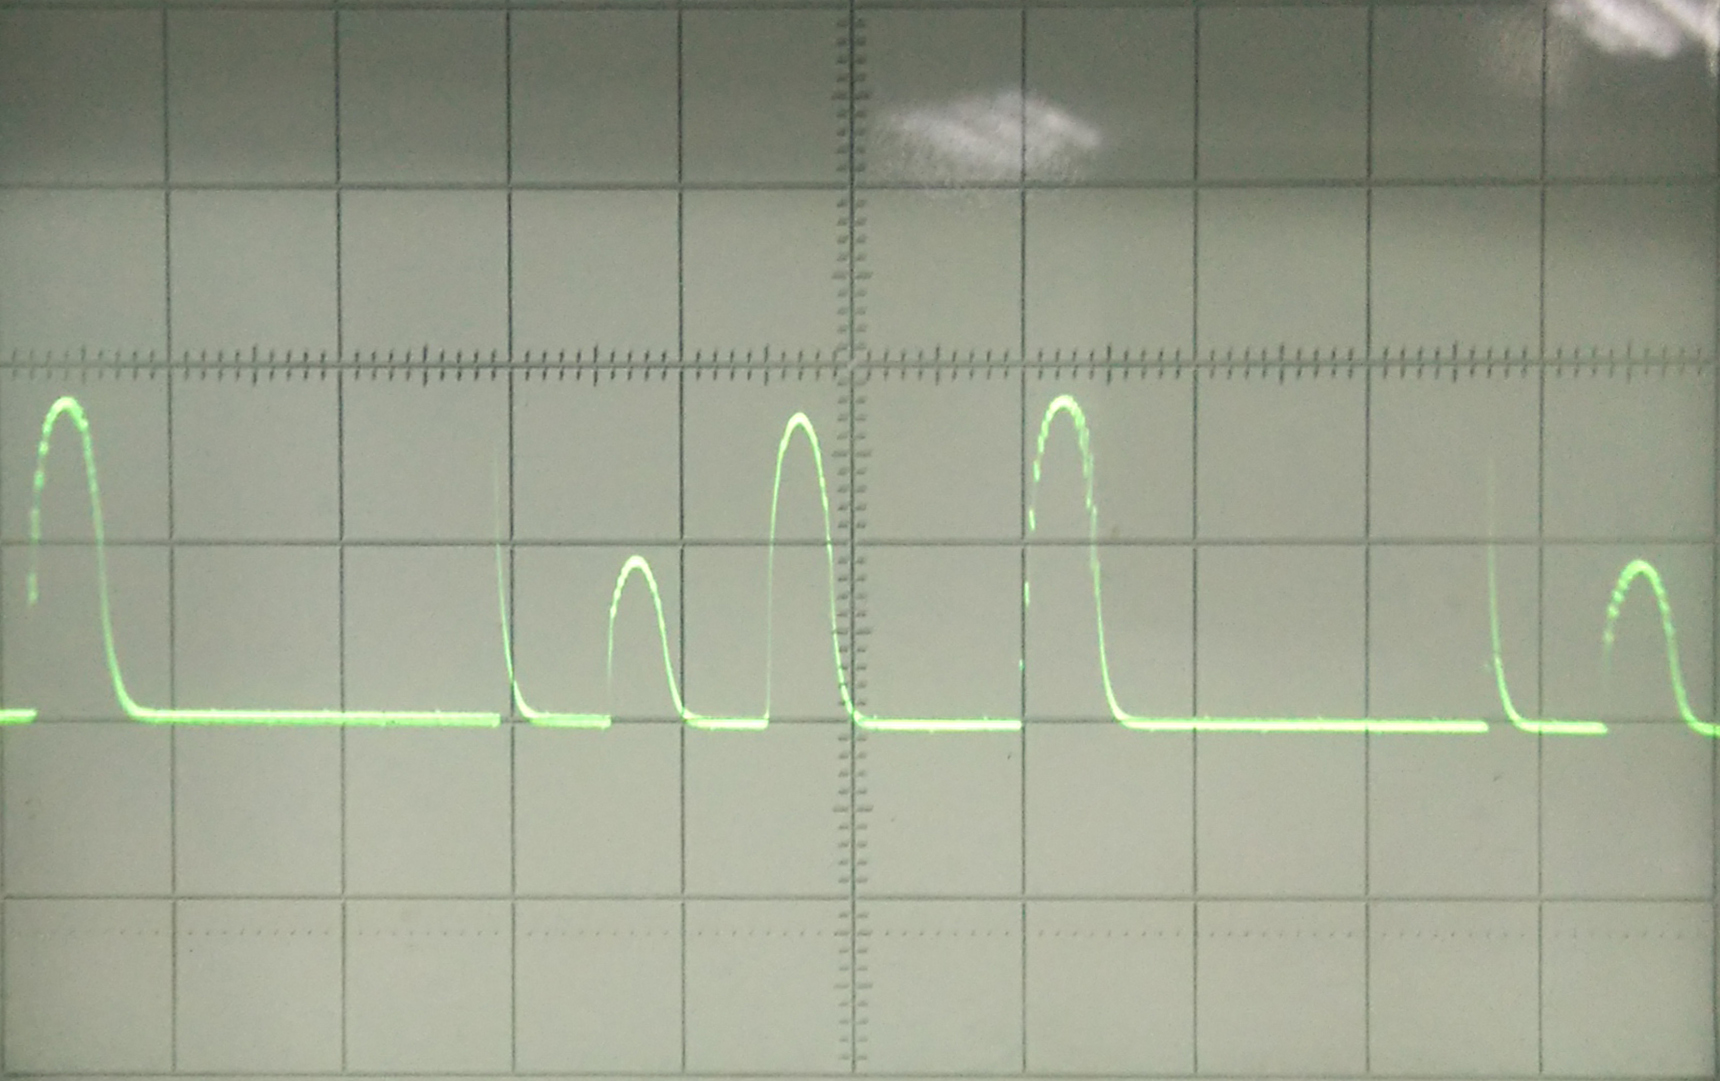
\includegraphics[width=\textwidth]{img/img4}}
    \caption{$U_{\text{уск}}=132$ В}
    \label{fig:img4}
  \end{minipage}
  \hfill
  \begin{minipage}[h]{0.45\textwidth}
    \centering
    {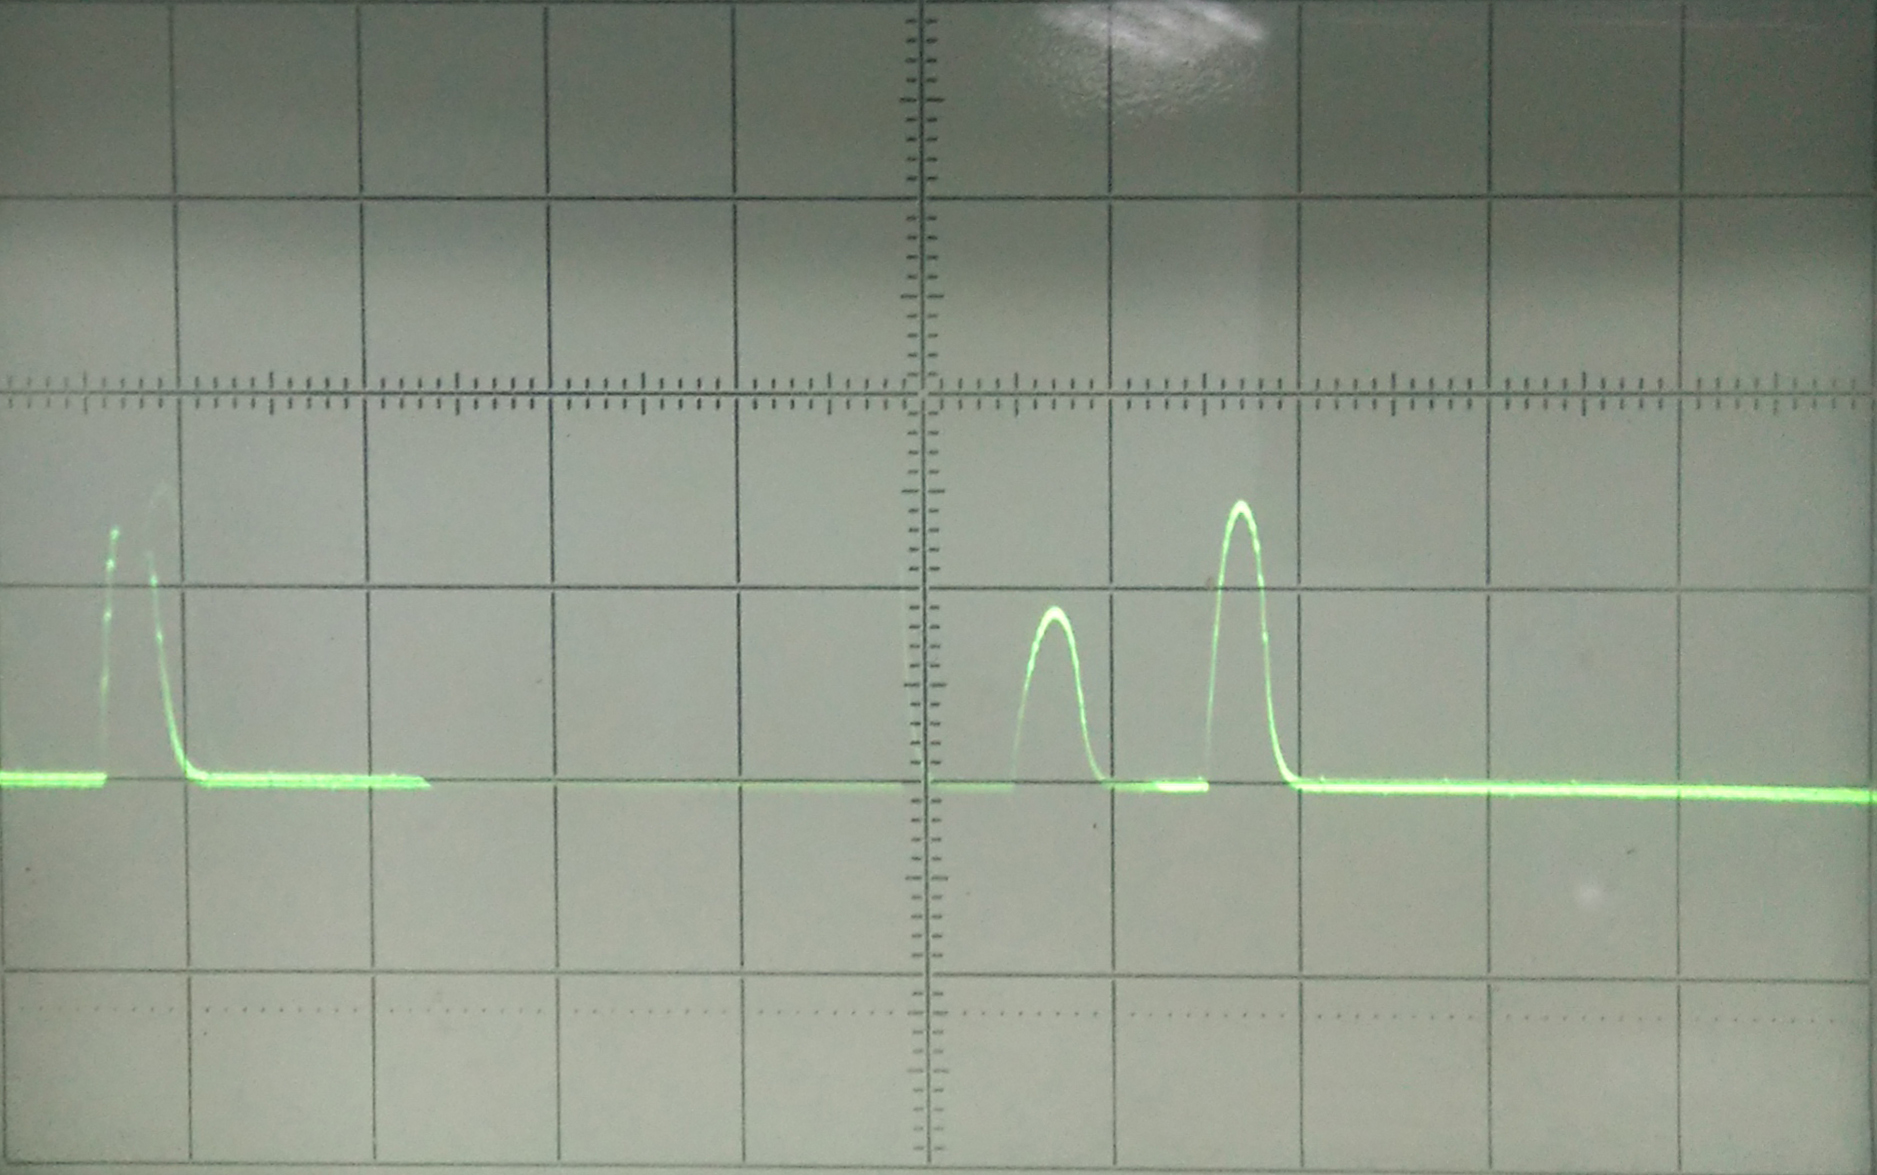
\includegraphics[width=\textwidth]{img/img5}}
    \caption{$U_{\text{уск}}=90$ В}
    \label{fig:img5}
  \end{minipage}

    \begin{minipage}[h]{0.45\textwidth}
    \centering
    {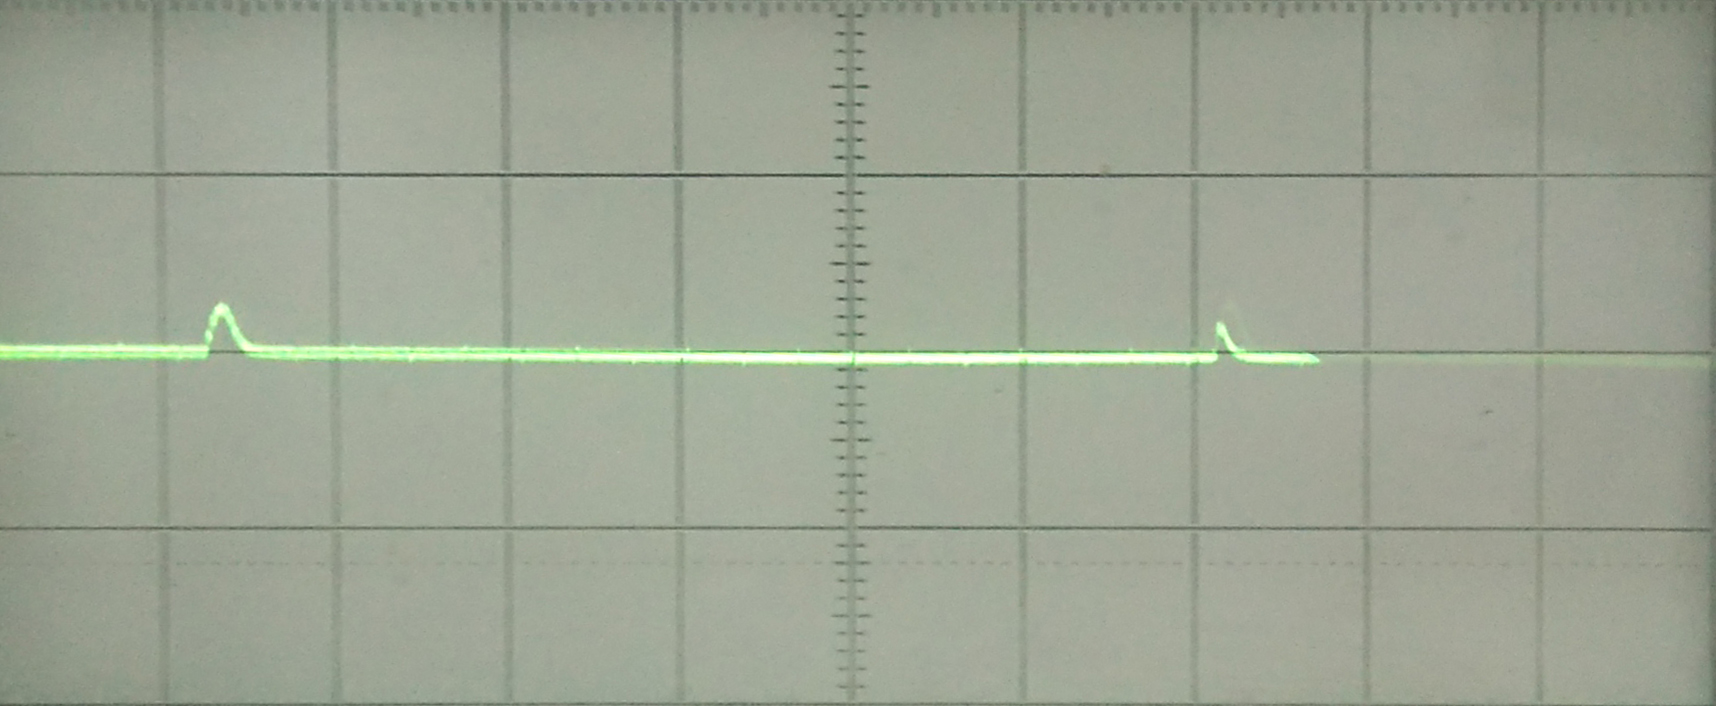
\includegraphics[width=\textwidth]{img/img6}}
    \caption{$U_{\text{уск}}=69$ В}
    \label{fig:img6}
  \end{minipage}
\end{figure}
\newpage


\begin{figure}[h]
  \begin{minipage}[h]{0.45\linewidth}
    \centering
    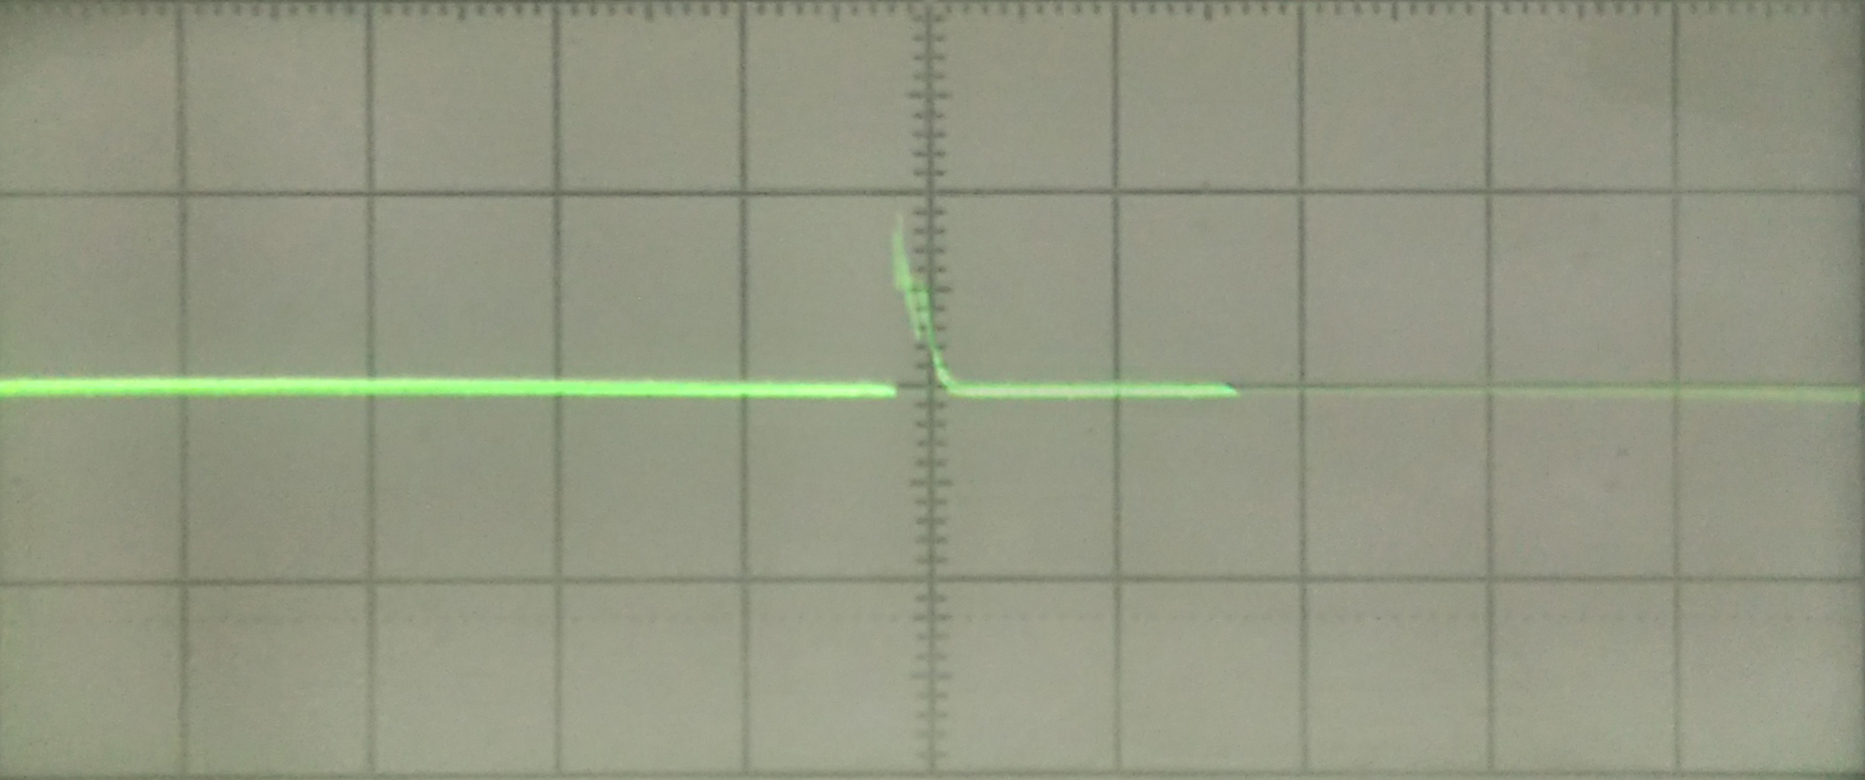
\includegraphics[width=\textwidth]{img/img7}
    \caption{$U_{\text{отр}}=108$ В}
    \label{fig:img7}
  \end{minipage}
  \hfill
  \begin{minipage}[h]{0.45\linewidth}
    \centering
    {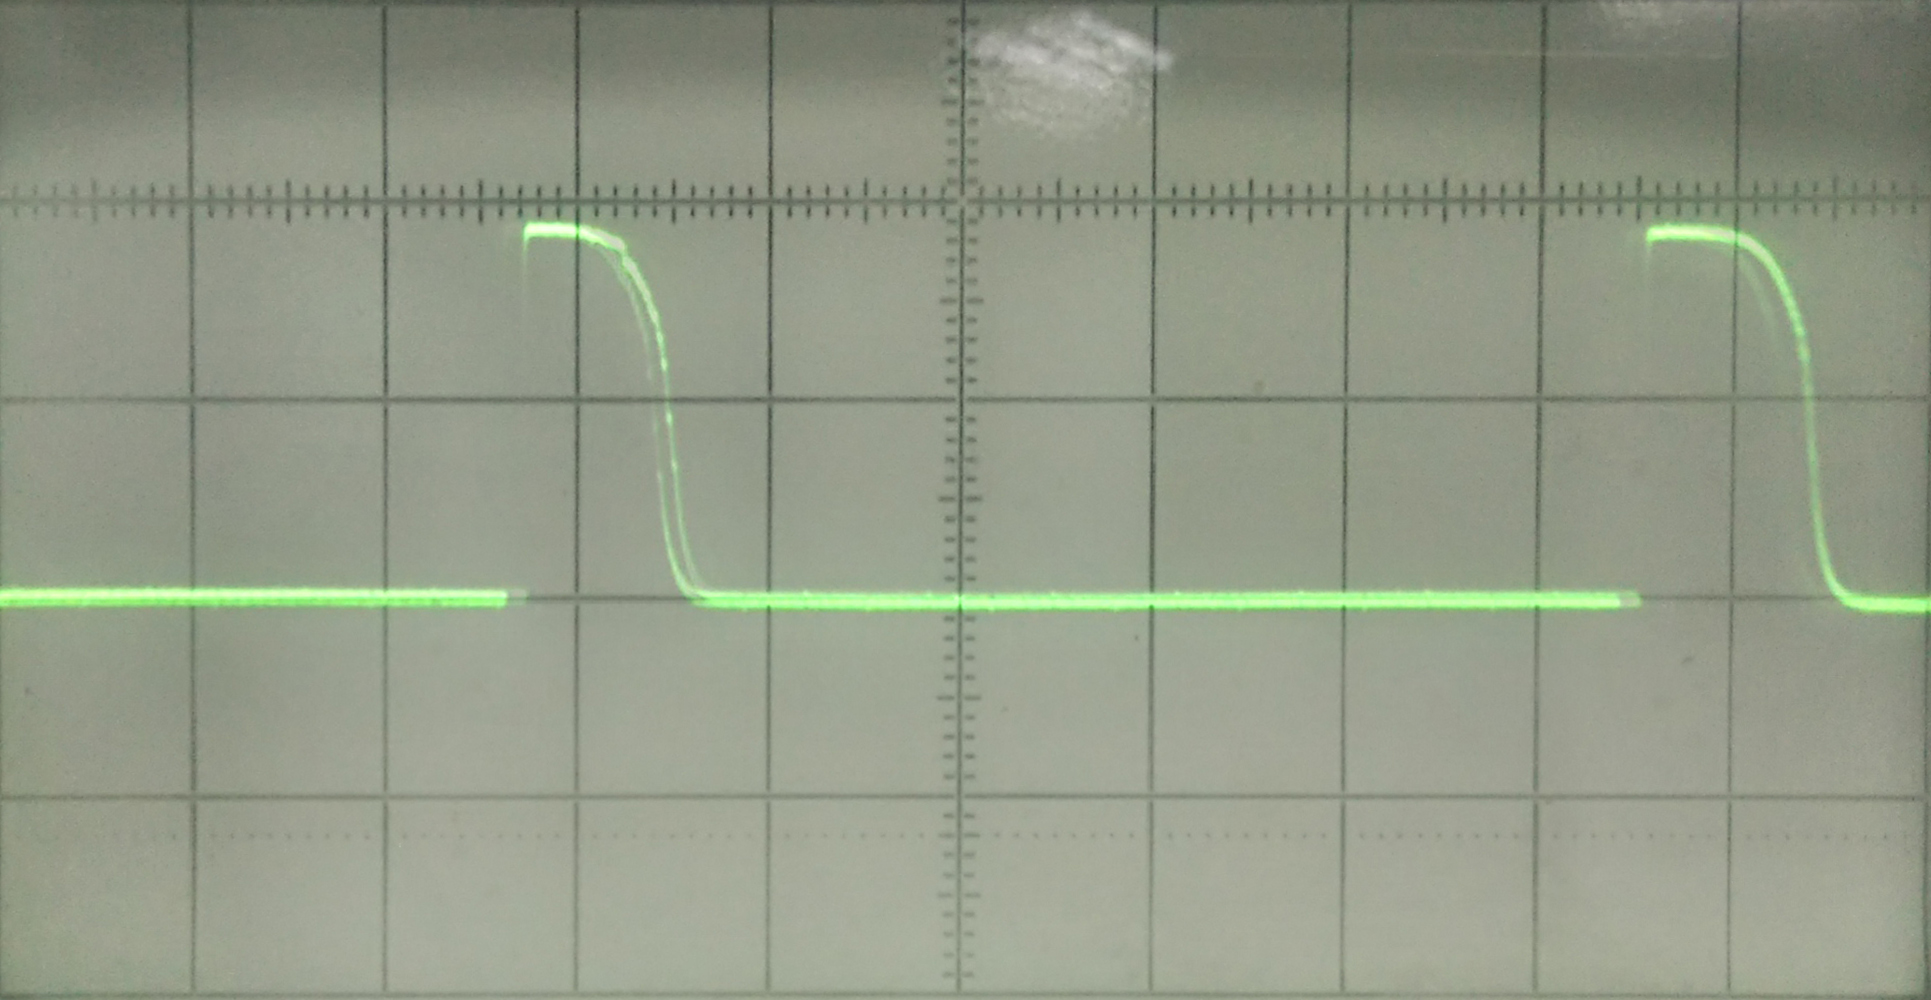
\includegraphics[width=\textwidth]{img/img8}}
    \caption{$U_{\text{отр}}=102$ В}
    \label{fig:img8}
  \end{minipage}
  \vfill
  \vspace{1em}
  \begin{minipage}[h]{0.45\linewidth}
    \centering
    {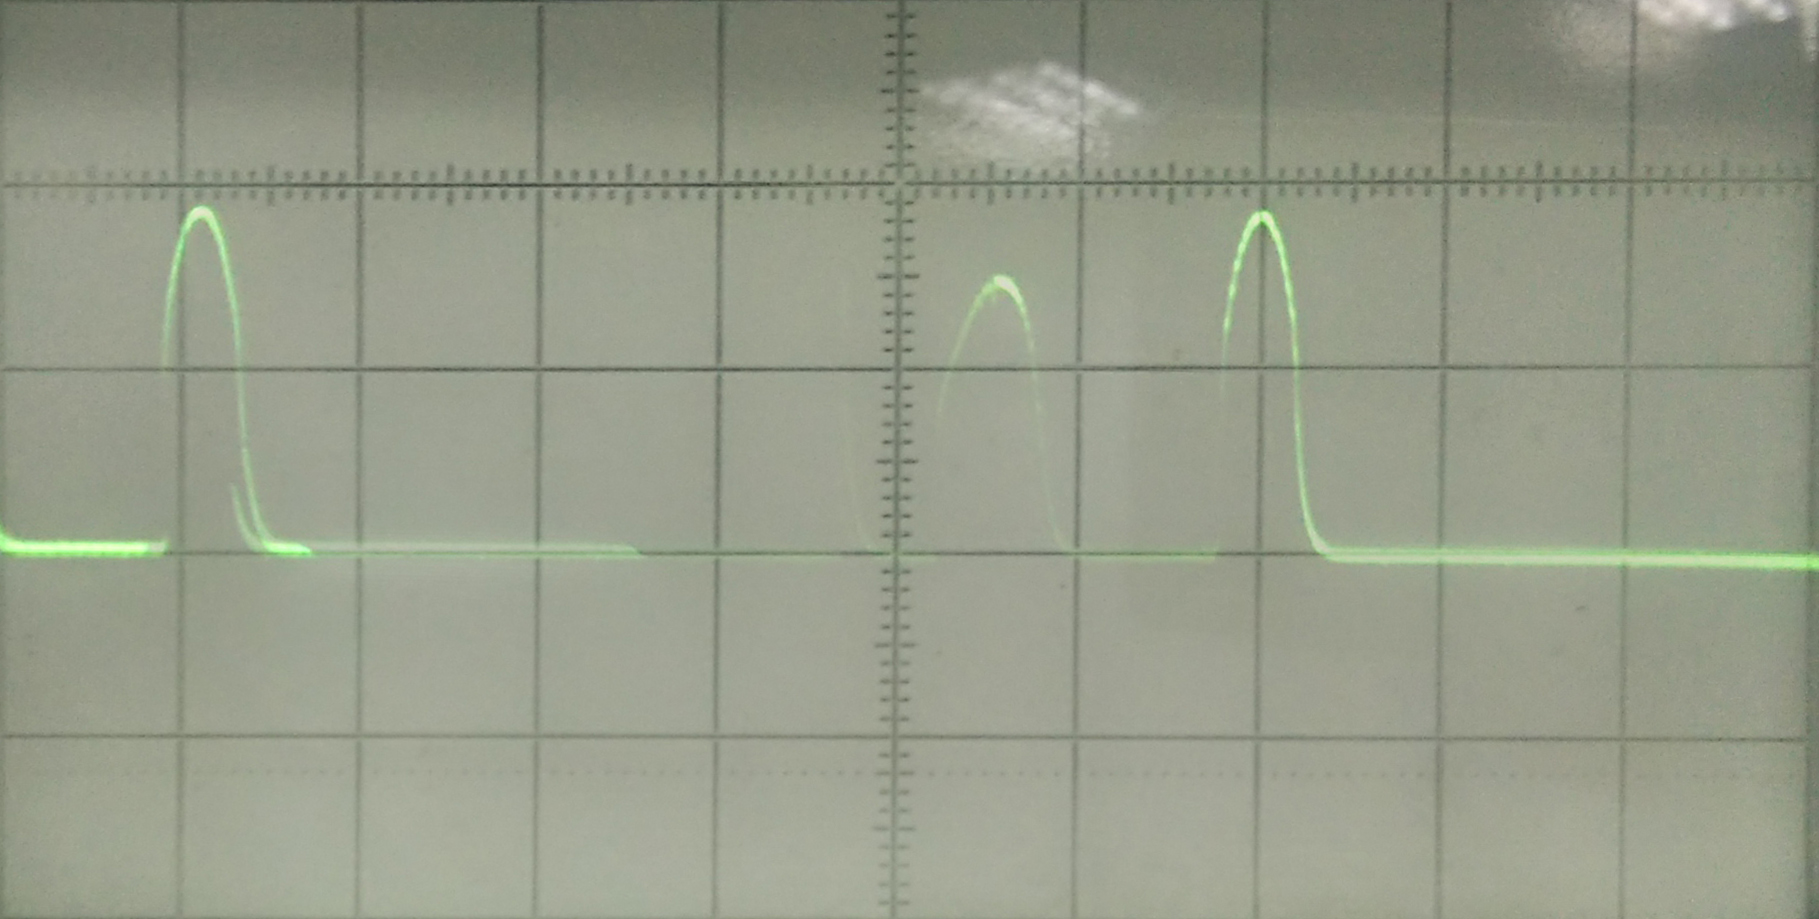
\includegraphics[width=\textwidth]{img/img9}}
    \caption{$U_{\text{отр}}=60$ В}
    \label{fig:img9}
  \end{minipage}
  \hfill
  \begin{minipage}[h]{0.45\textwidth}
    \centering
    {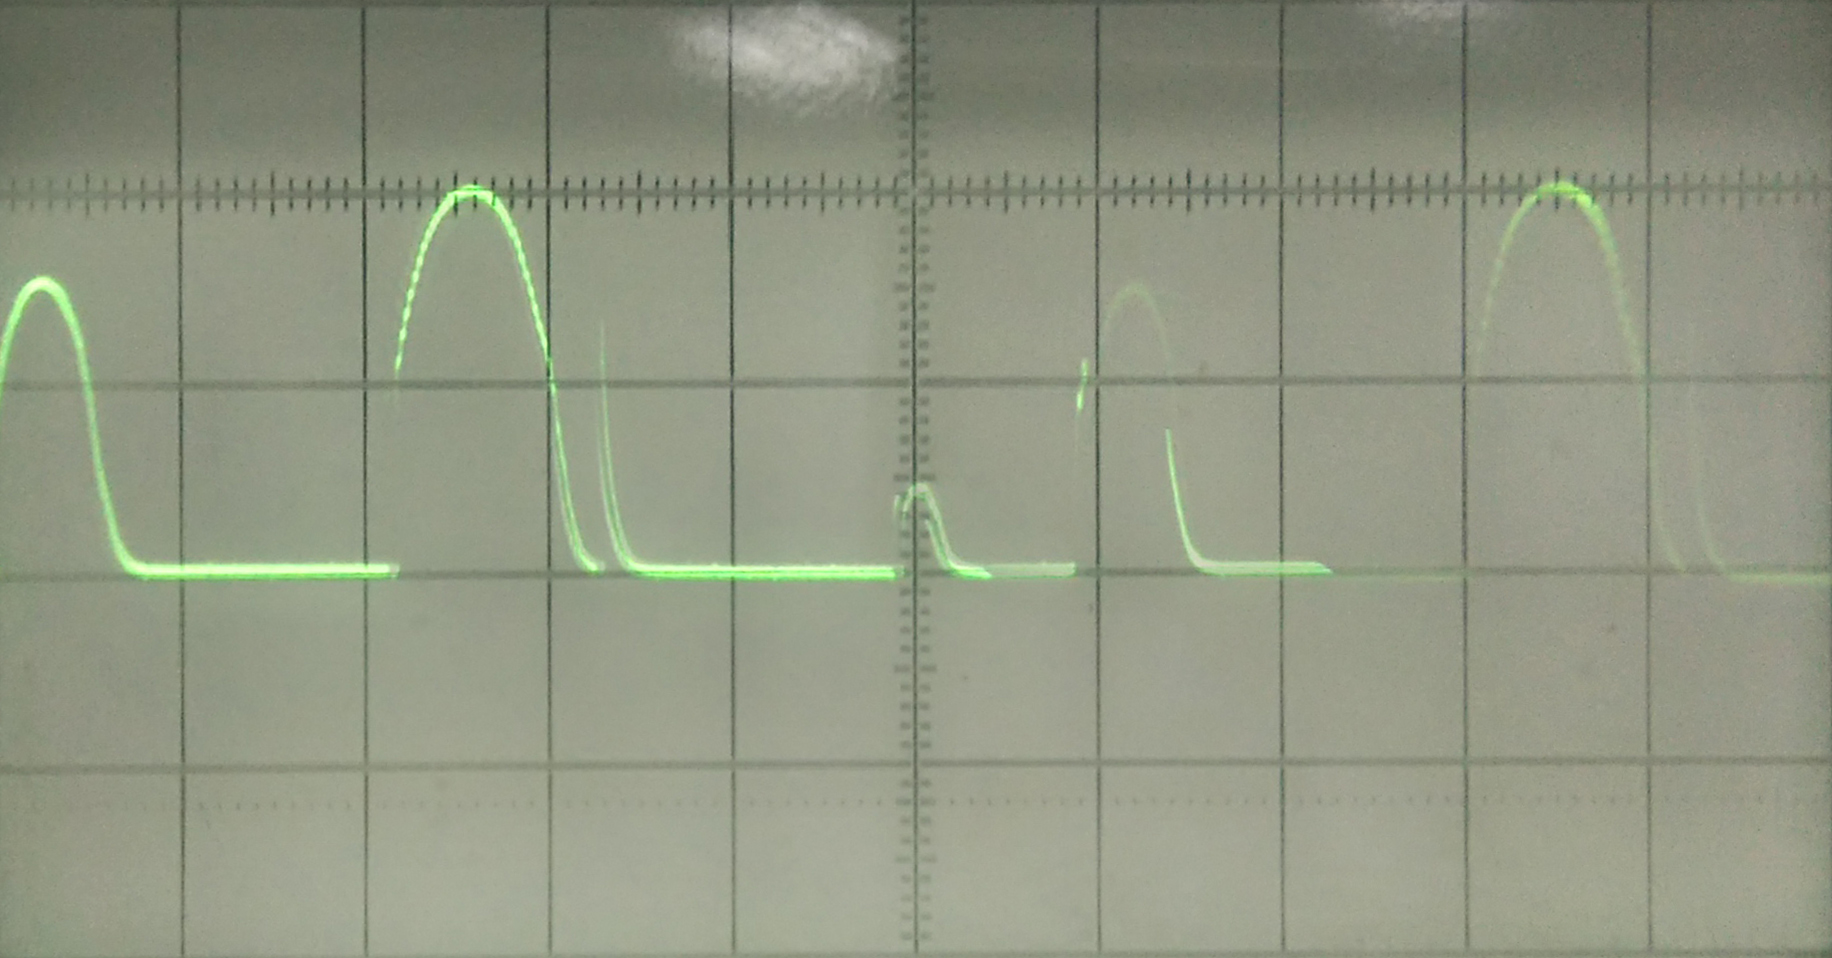
\includegraphics[width=\textwidth]{img/img10}}
    \caption{$U_{\text{отр}}=24$ В}
    \label{fig:img10}
  \end{minipage}

    \begin{minipage}[h]{0.45\textwidth}
    \centering
    {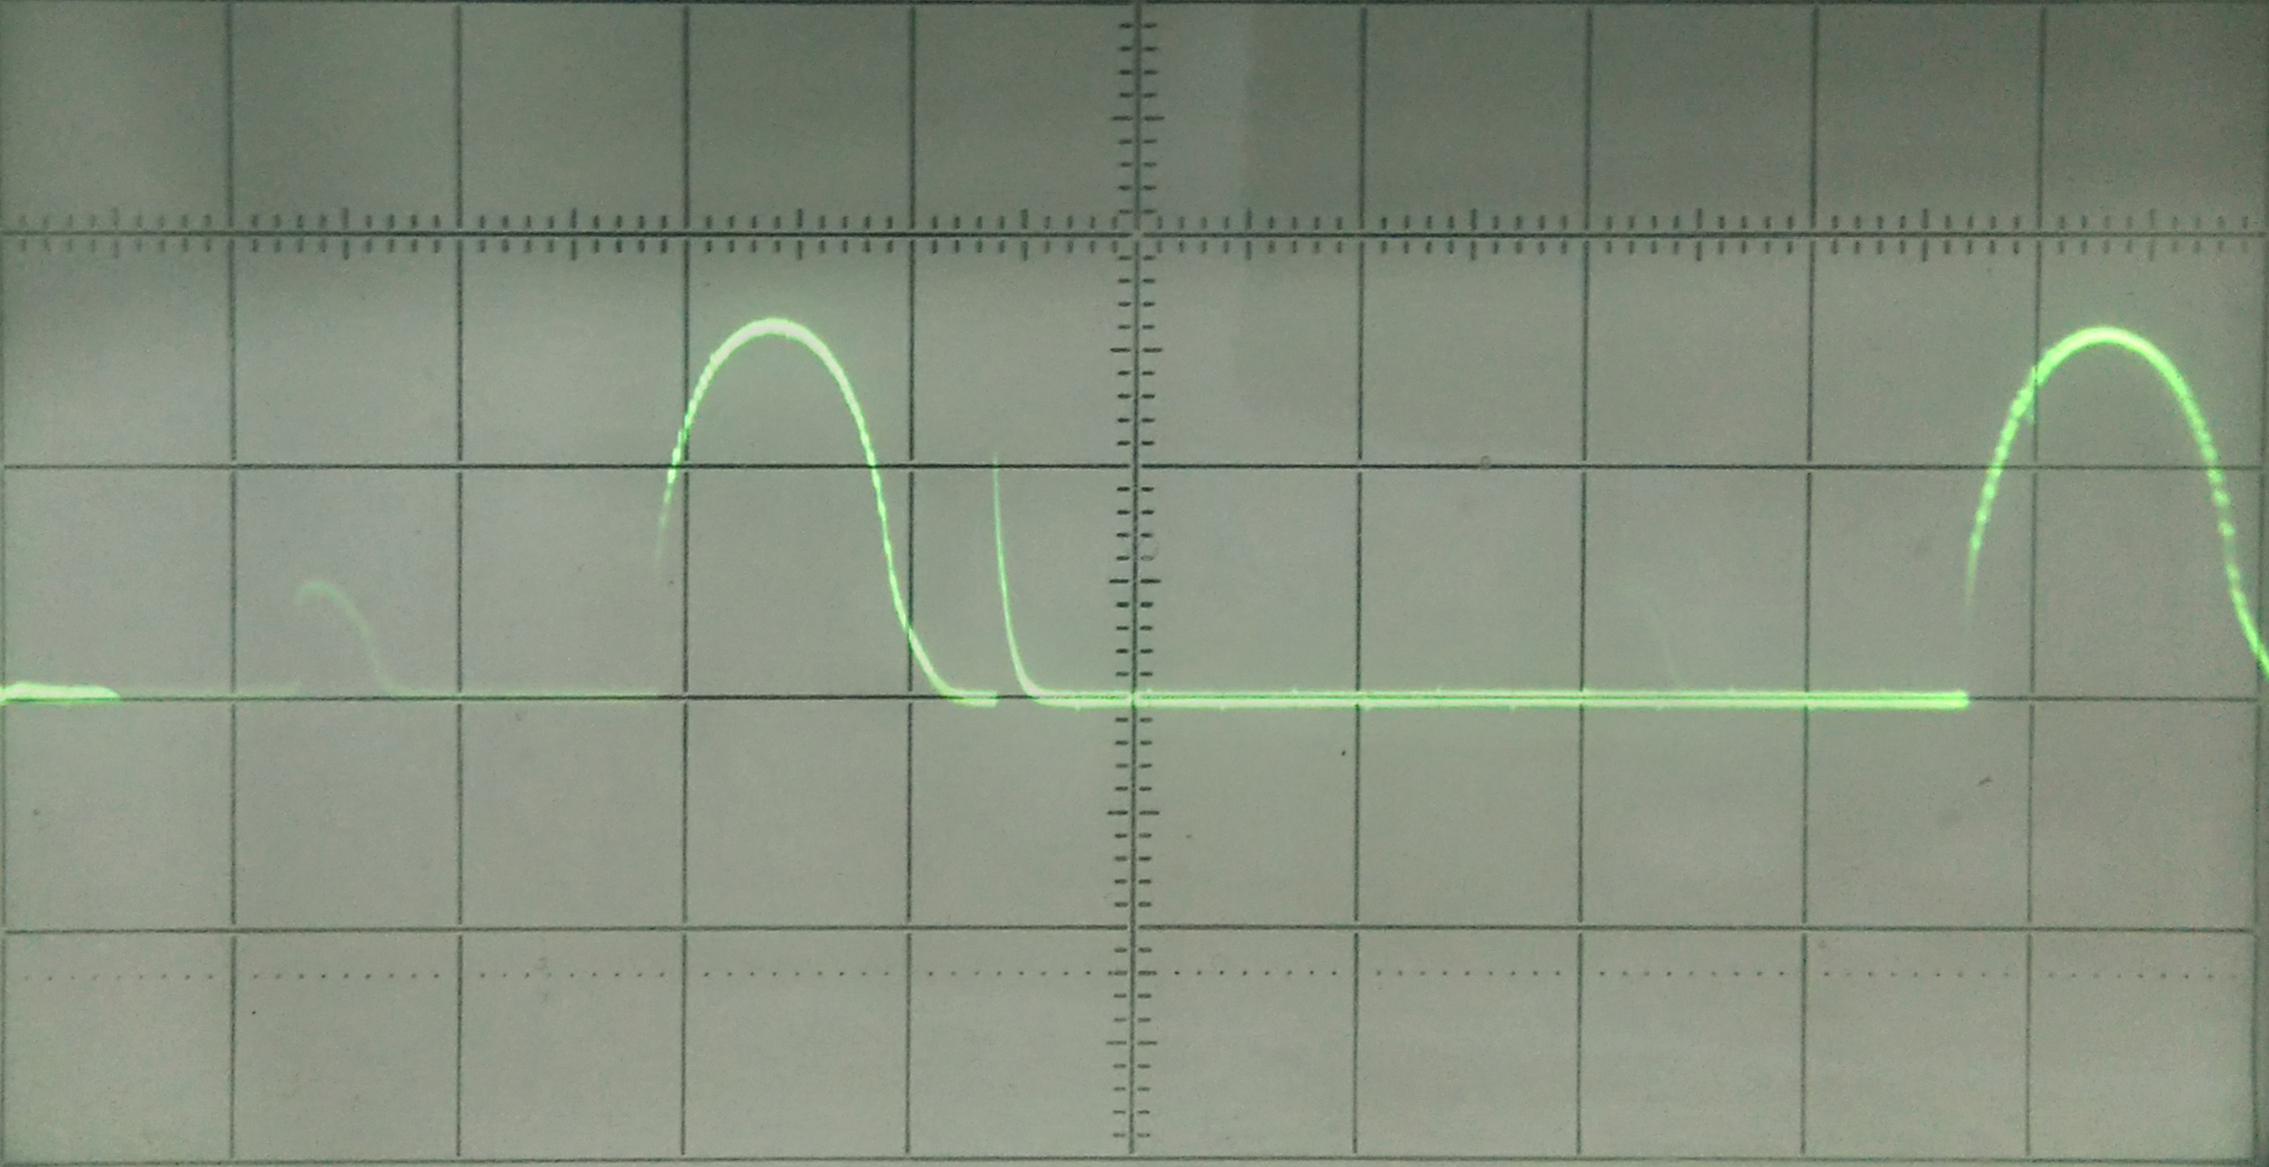
\includegraphics[width=\textwidth]{img/img11}}
    \caption{$U_{\text{отр}}=6$ В}
    \label{fig:img11}
  \end{minipage}
\end{figure}
На рис. \ref{fig:img2}-\ref{fig:img6}  и рис.\ref{fig:img7}-\ref{fig:img11} - показано, как меняются зоны при уменьшении $U_{\text{уск}}$ и $U_{\text{отр}}$ соответственно. 

%\newpage
Ширина частотной перестройки клистрона для трех зон генерации.

Для первой зоны она составила $\lambda_1=10.58-10.55=0.03$ см.

Для второй зоны -- $\lambda_2=10.6-10.515=0.085$ см.

Для третьей зоны -- $\lambda_3=10.58-10.515=0.065$ см.
\subsection{Задание 3 и 4}
% \subsubsection{Зависимость тока в цепи детектора от напряжения на отражателе}

% \begin{figure}[H]
%     \centering
%     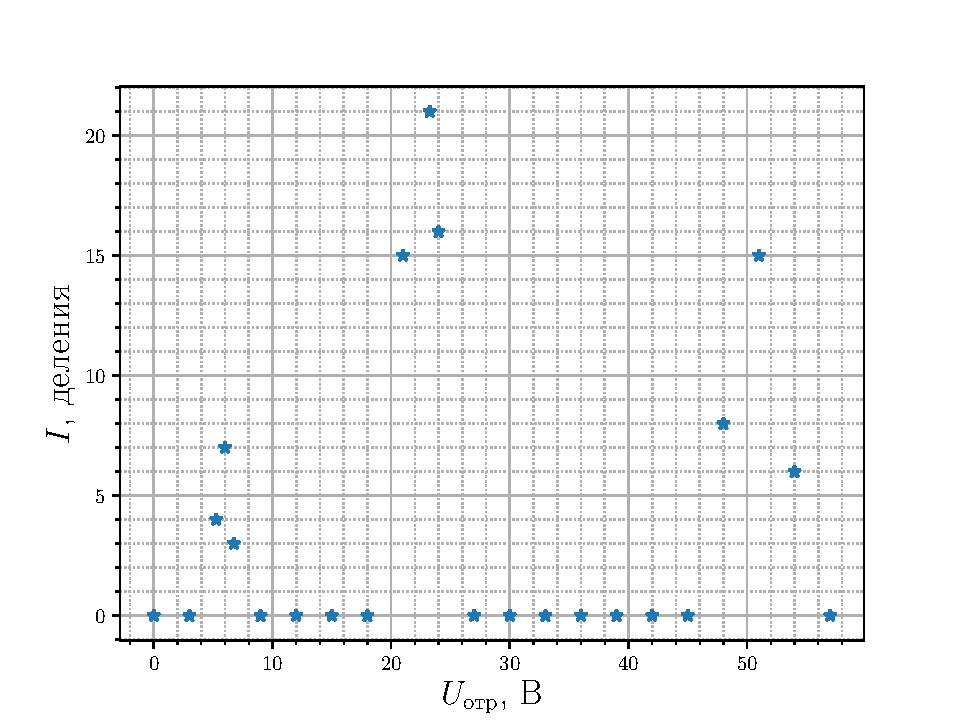
\includegraphics[height=0.4\textheight]{fig/res90V_1}
%     \caption{$U_{\text{отр}}=90$ В}
%     \label{fig:res90V_1}
% \end{figure}
% \begin{figure}[H]
%     \centering
%     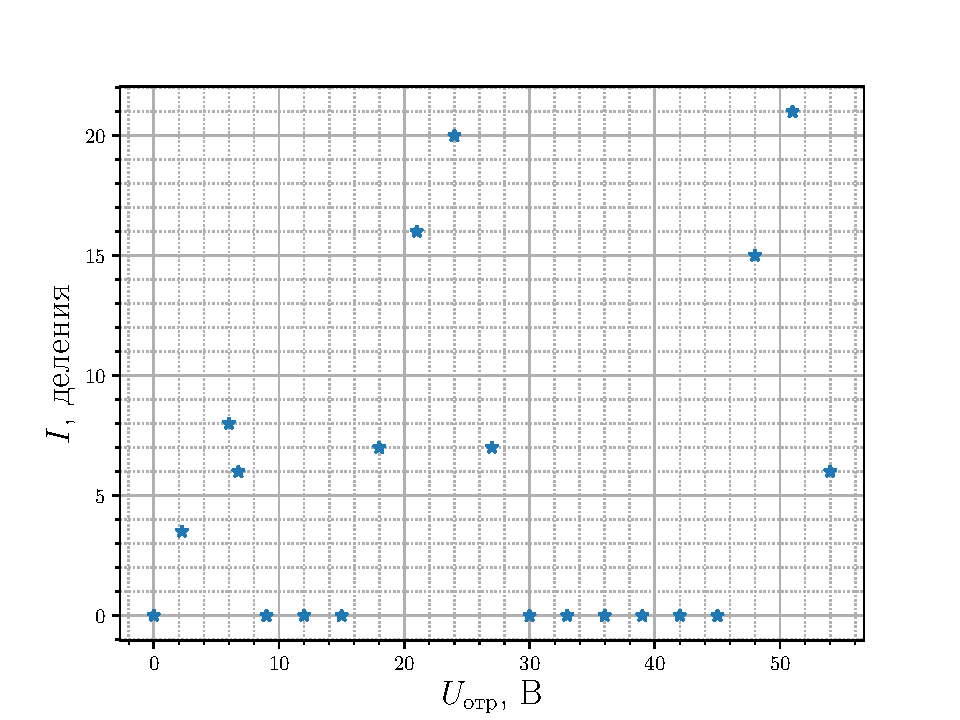
\includegraphics[height=0.4\textheight]{fig/res96V_1}
%     \caption{$U_{\text{отр}}=96$ В}
%     \label{fig:res96V_1}
% \end{figure}
% \begin{figure}[H]
%     \centering
%     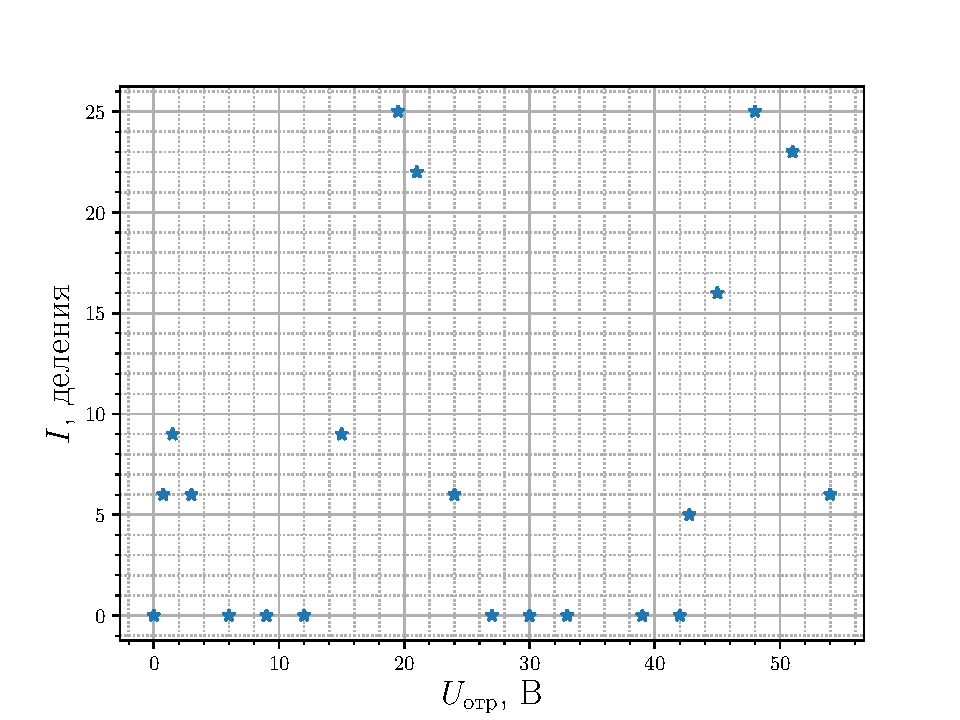
\includegraphics[height=0.4\textheight]{fig/res120V_1}
%     \caption{$U_{\text{отр}}=120$ В}
%     \label{fig:res120V_1}
% \end{figure}

\begin{figure}[H]
    \centering
    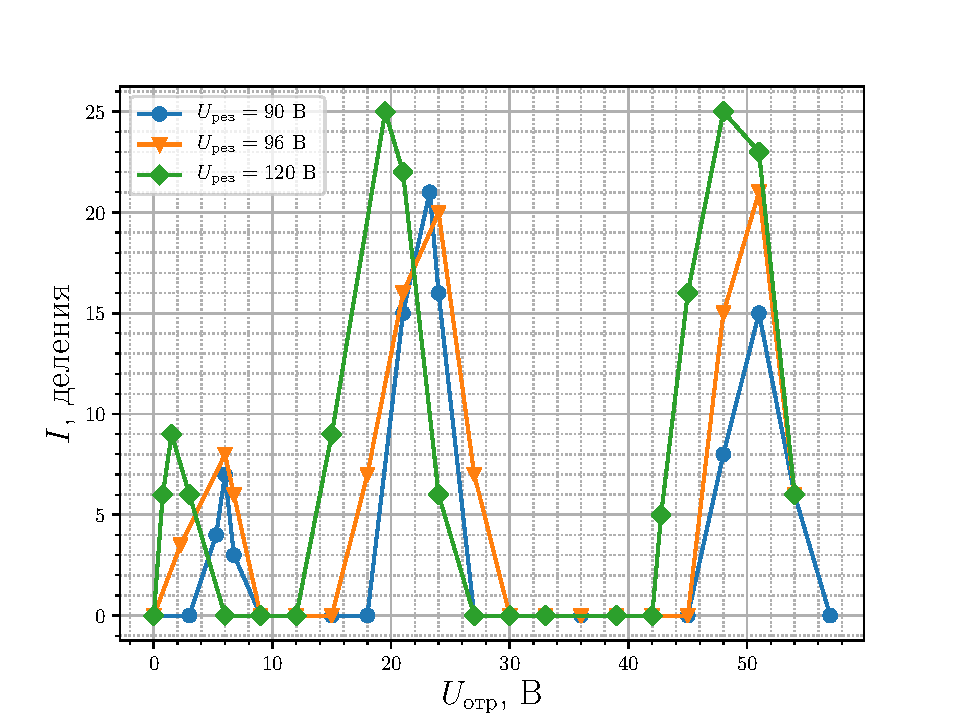
\includegraphics[width=\linewidth]{fig/task3a}
    \caption{Зависимость тока в цепи детектора от напряжения на отражателе}
    \label{fig:task3a}
\end{figure}
 
 Из графиков видно, что чем ниже номер зоны генерации, тем шире сама зона. В условии возбуждения клистрона величина $\theta _ { \text{г} }$ зависит от напряжения отражателя:

  $$\theta _ { \text{г} } = \frac { 2 m } { e } \frac { v _ { 0 } \omega L } { U _ { 0 } - U _ { \text{ oтр } } }.$$ 
  Здесь $U_{\text{отр}}<0$. Это значит, что чем больше по модулю $U_{\text{отр}}$, тем меньше $\theta _ { \text{г} }$ и больший диапазон $\theta _ { \text{г} }$ может убраться между $\pi+ 2\pi n$ и $2\pi(n+1)$.

\begin{figure}[H]
    \centering
    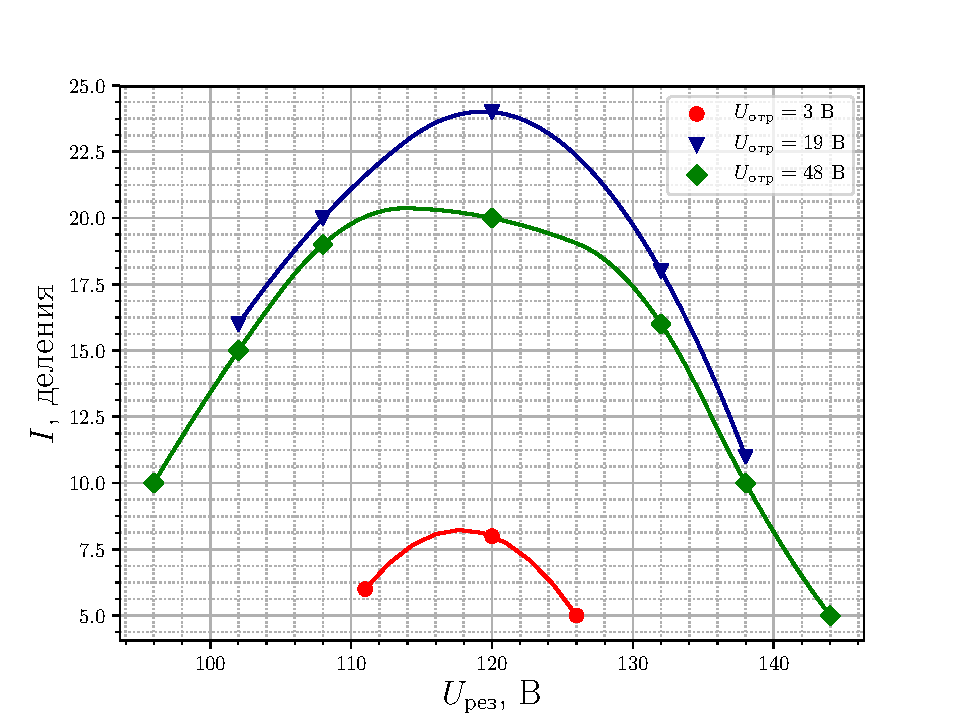
\includegraphics[width=\linewidth]{fig/task3b}
    \caption{Зависимость тока в цепи детектора от напряжения на отражателе}
    \label{fig:task3b}
\end{figure}


В центре каждой зоны генерации поток отдает резонатору наибольшую мощность $\displaystyle P_{max}\sim I_1 U_m \sim \frac{2I_0 XJ_1(X) U_0}{\theta _ { \text{г} }}$, где $J_1(X)$ - функция Бесселя первого порядка. Первая гармоника конвекционного тока достигает максимума при $X=1.84$. Следовательно, активная мощность, отдаваемая электронным потоком резонатору, достигает максимума в любой зоне генерации при $X=1.84$. Это, в частности, означает, что колебательное напряжение на зазоре $U_m$, соответствующее максимуму электронной мощности, возрастает с уменьшением номера зоны. В соответствии с выражением для максимальной мощности, с уменьшением номера зоны возрастают также и абсолютные значения максимумов электронной мощности. $$U_m=\frac{2U_0X}{M\theta _ { \text{г} }}=\frac{1.84 U_o}{\pi M(n+\frac 34)n}$$

%\newpage
% \subsubsection{Зависимость тока в цепи детектора от напряжения на резонаторе}
% \begin{figure}[H]
%     \centering
%     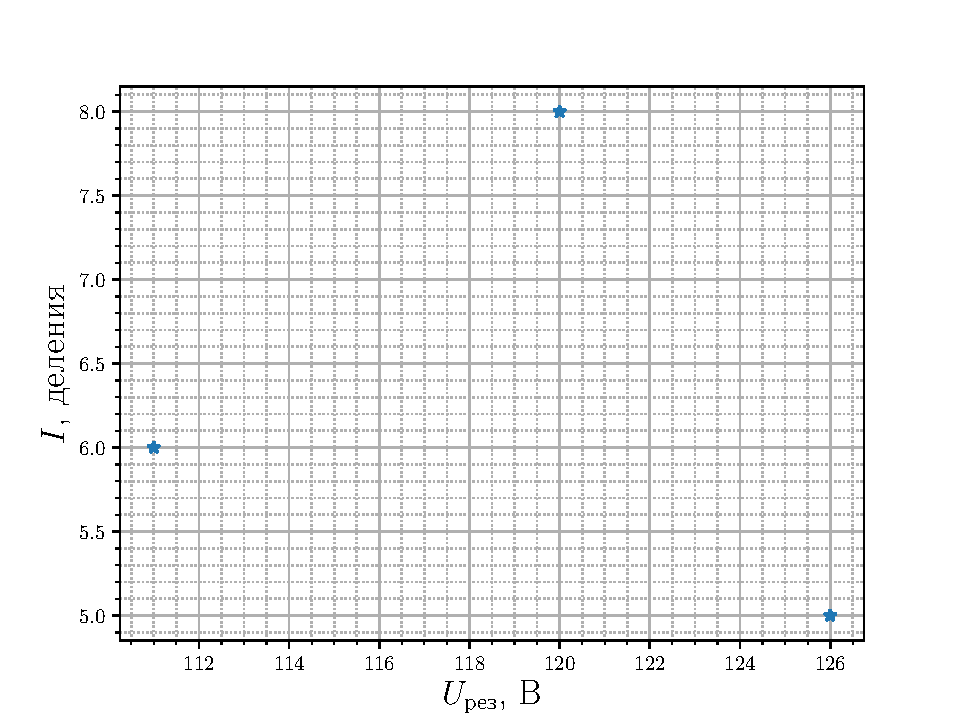
\includegraphics[height=0.4\textheight]{fig/ref3V_1}
%     \caption{$U_{\text{рез}}=3$ В}
%     \label{fig:ref3V_2}
% \end{figure}
% \begin{figure}[H]
%     \centering
%     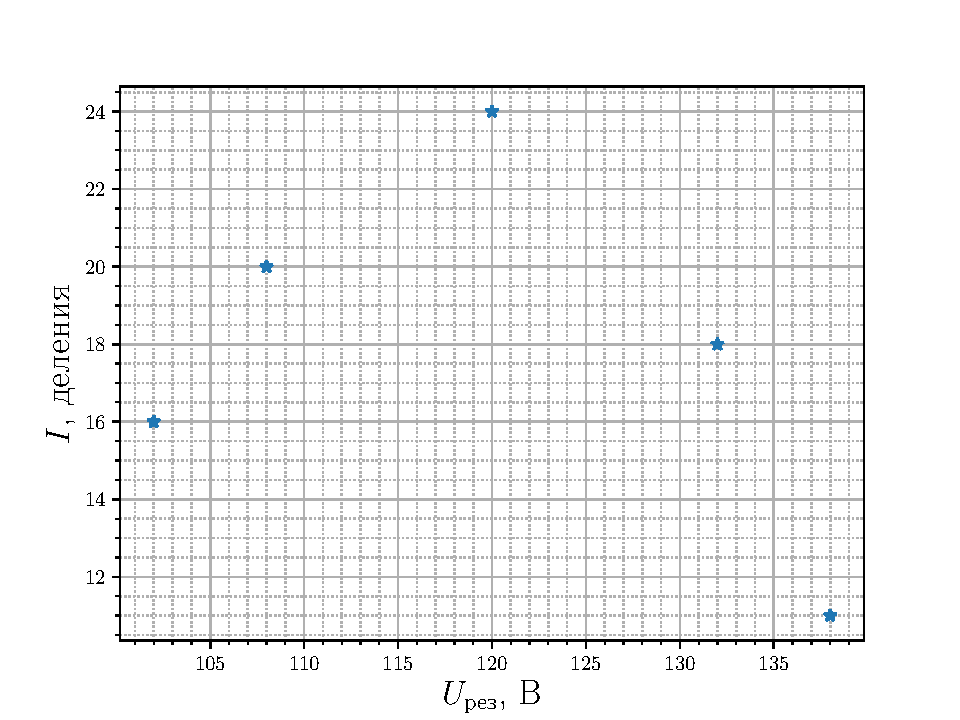
\includegraphics[height=0.4\textheight]{fig/ref19V_1}
%     \caption{$U_{\text{рез}}=19$ В}
%     \label{fig:ref19V_2}
% \end{figure}
% \begin{figure}[H]
%     \centering
%     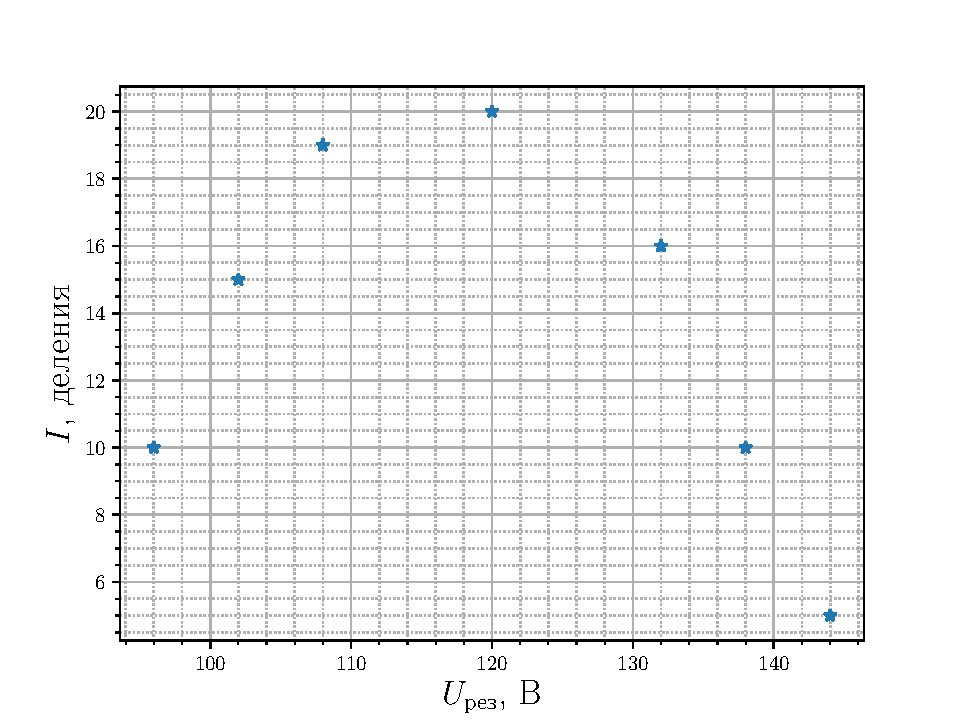
\includegraphics[height=0.4\textheight]{fig/ref48V_1}
%     \caption{$U_{\text{рез}}=48$ В}
%     \label{fig:ref48V_2}
% \end{figure}
\begin{figure}[H]
    \centering
    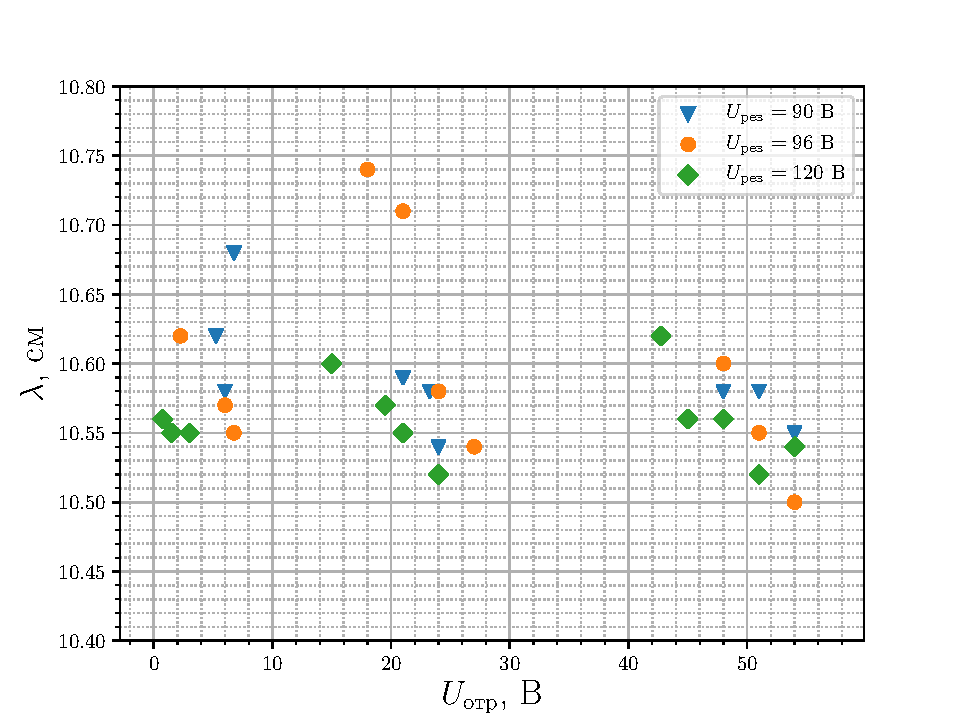
\includegraphics[width=\linewidth]{fig/task4a}
    \caption{Зависимость длины волны от напряжения на отражателе}
    \label{fig:task4a}
\end{figure}

При увеличении абсолютной величины $U_{\text{отр}}$ происходит рост частоты генерации клистрона. 

\begin{figure}[H]
    \centering
    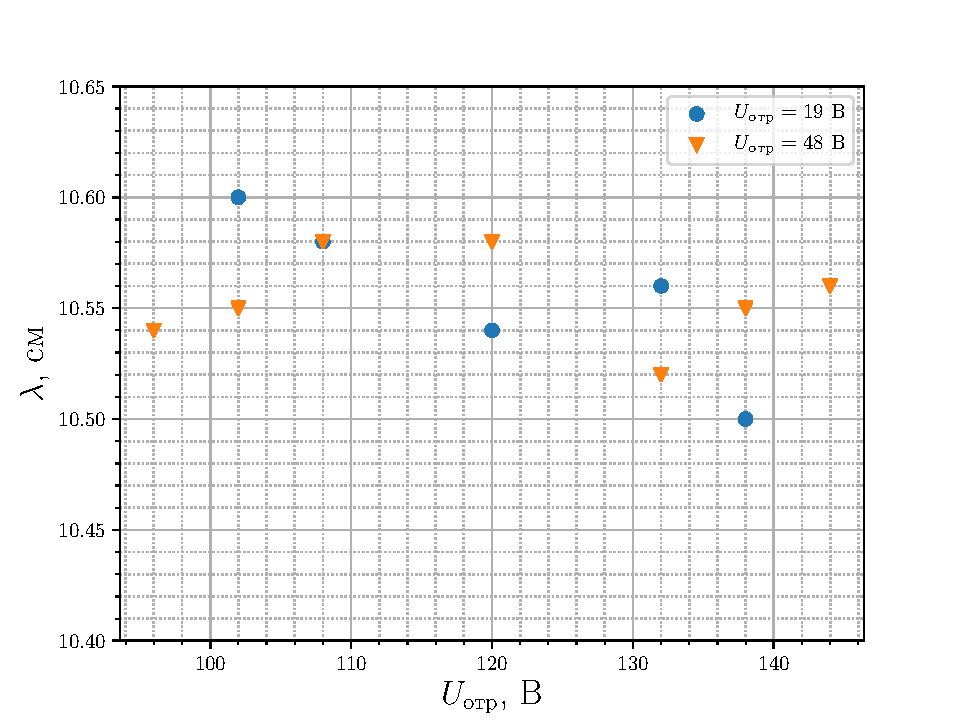
\includegraphics[width=\linewidth]{fig/task4b}
    \caption{Зависимость тока в цепи детектора от напряжения на резонаторе}
    \label{fig:task4b}
\end{figure}

% \subsection{Задание 4}
% %\newpage
% \subsubsection{Зависимость длины волны от напряжения на отражателе}

% \begin{figure}[H]
%     \centering
%     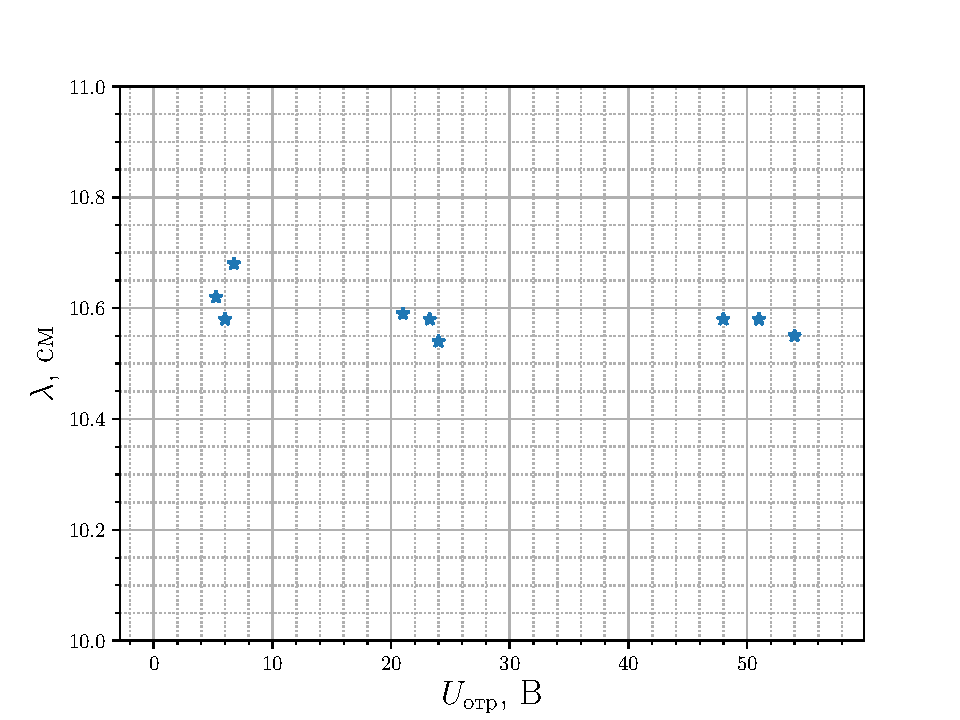
\includegraphics[height=0.4\textheight]{fig/res90V_2}
%     \caption{$U_{\text{отр}}=90$ В}
%     \label{fig:res90V_2}
% \end{figure}
% \begin{figure}[H]
%     \centering
%     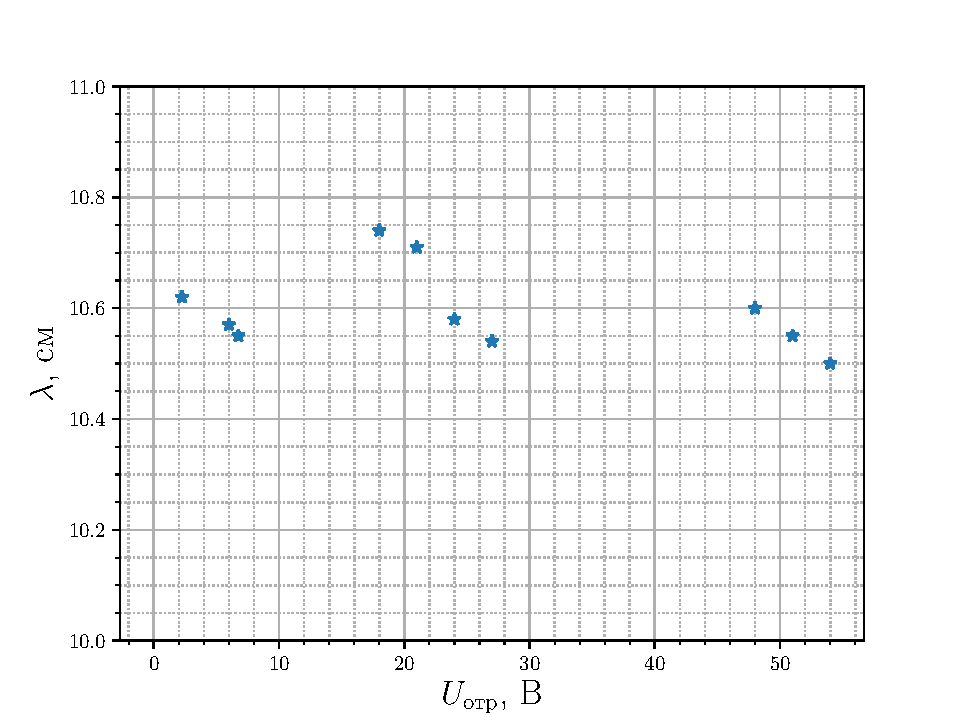
\includegraphics[height=0.4\textheight]{fig/res96V_2}
%     \caption{$U_{\text{отр}}=96$ В}
%     \label{fig:res96V_2}
% \end{figure}
% \begin{figure}[H]
%     \centering
%     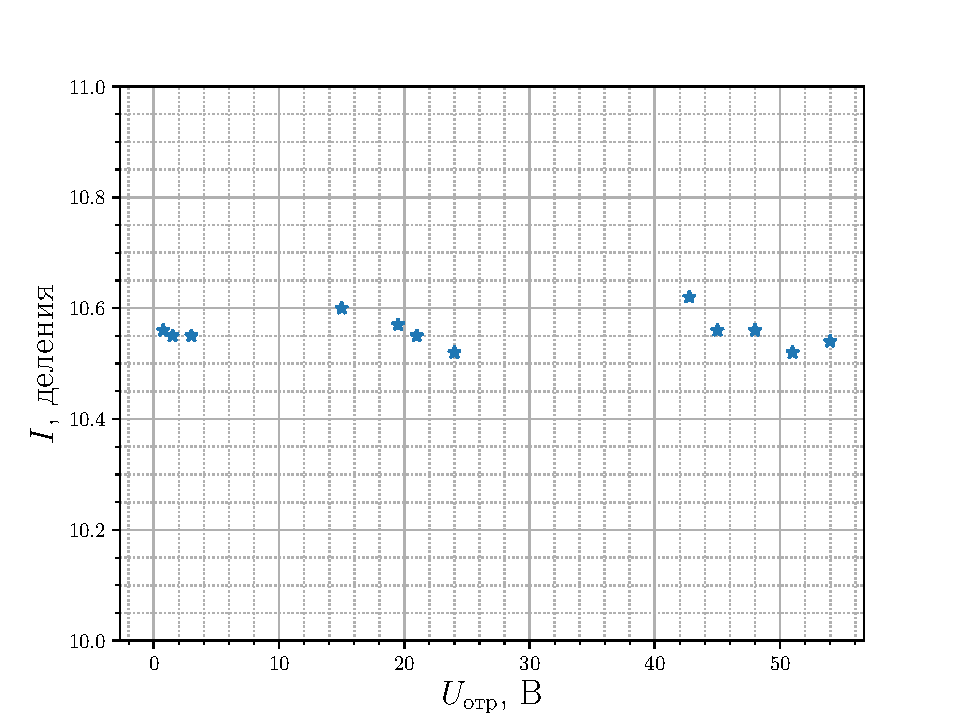
\includegraphics[height=0.4\textheight]{fig/res120V_2}
%     \caption{$U_{\text{отр}}=120$ В}
%     \label{fig:res120V_2}
% \end{figure}

%\newpage
% \subsubsection{Зависимость длины волны от напряжения на резонаторе}

% \begin{figure}[H]
%     \centering
%     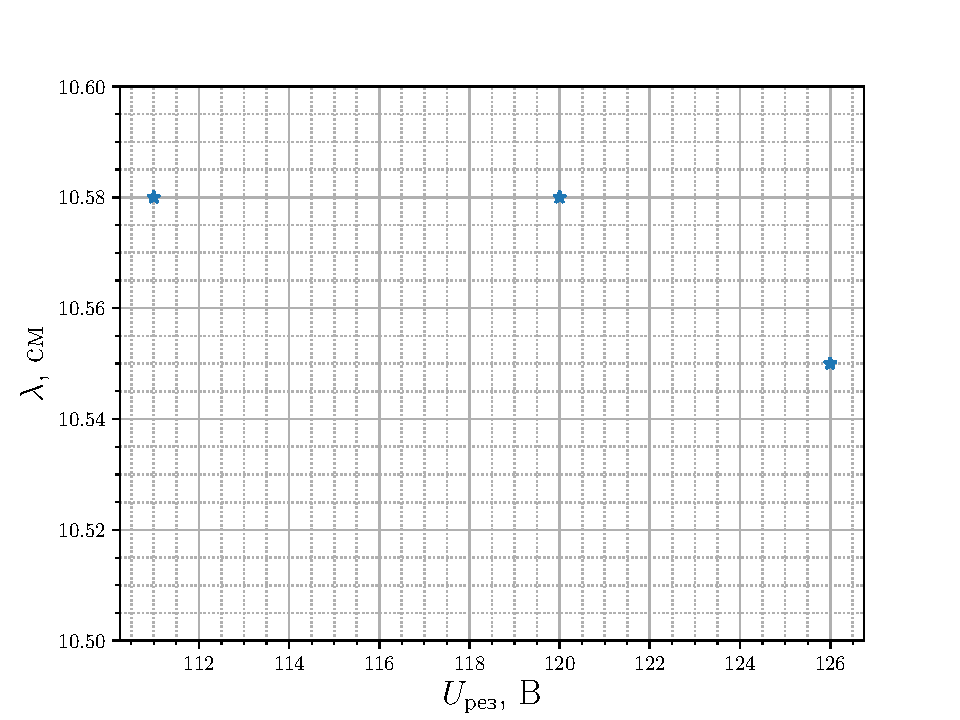
\includegraphics[height=0.4\textheight]{fig/ref3V_2}
%     \caption{$U_{\text{рез}}=3$ В}
%     \label{fig:ref3V_2}
% \end{figure}
% \begin{figure}[H]
%     \centering
%     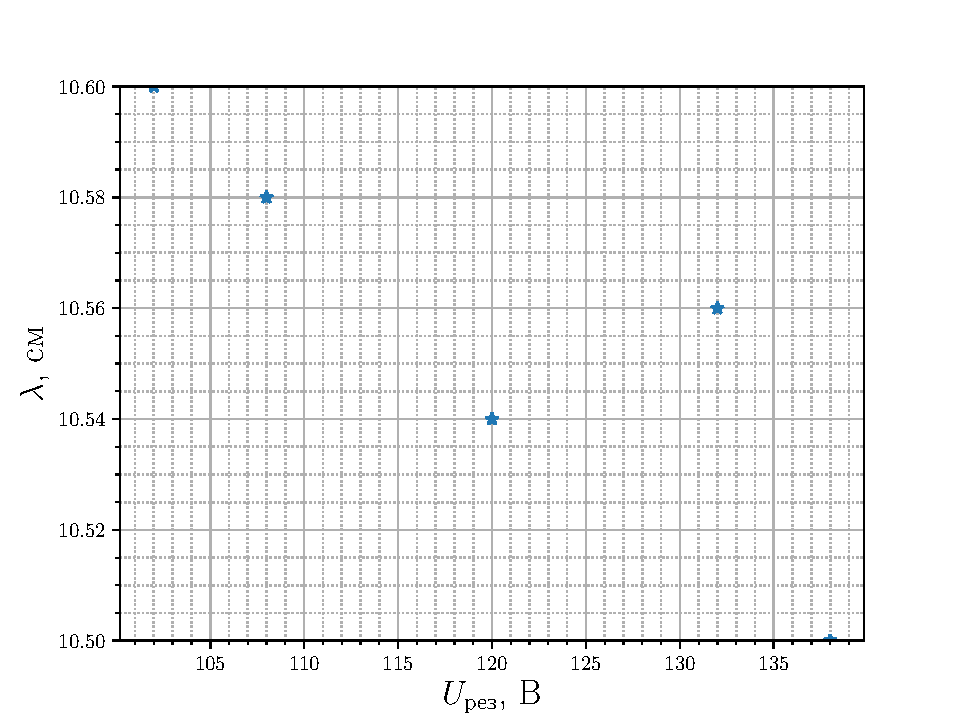
\includegraphics[height=0.4\textheight]{fig/ref19V_2}
%     \caption{$U_{\text{рез}}=19$ В}
%     \label{fig:ref19V_2}
% \end{figure}
% \begin{figure}[H]
%     \centering
%     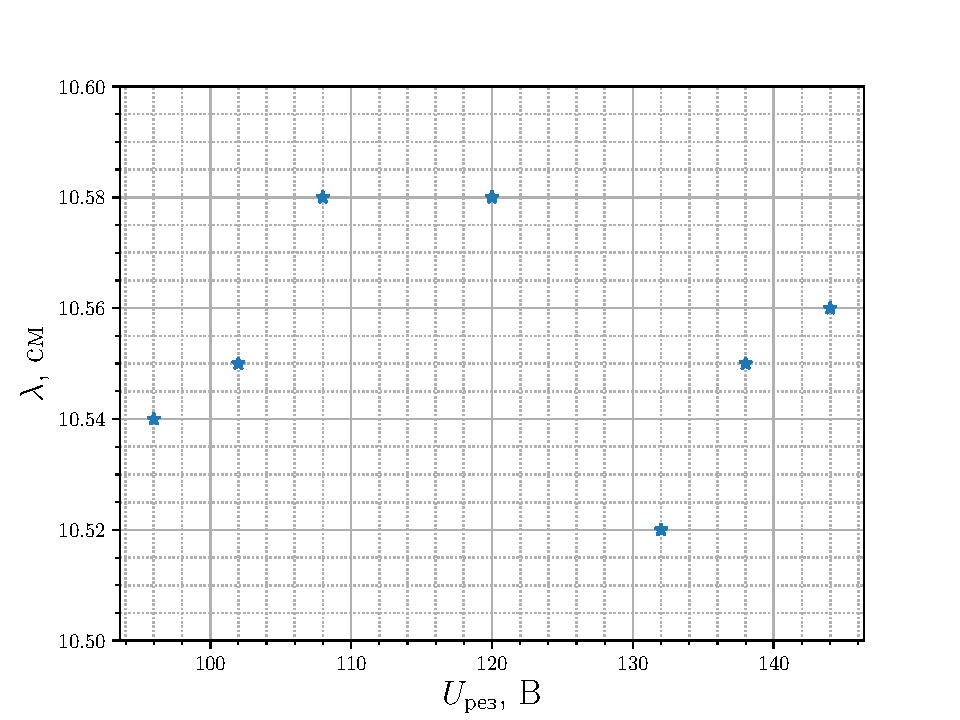
\includegraphics[height=0.4\textheight]{fig/ref48V_2}
%     \caption{$U_{\text{рез}}=48$ В}
%     \label{fig:ref48V_2}
% \end{figure}

%\newpage
\subsection{Задание 5}
% \begin{figure}[H]
%     \centering
%     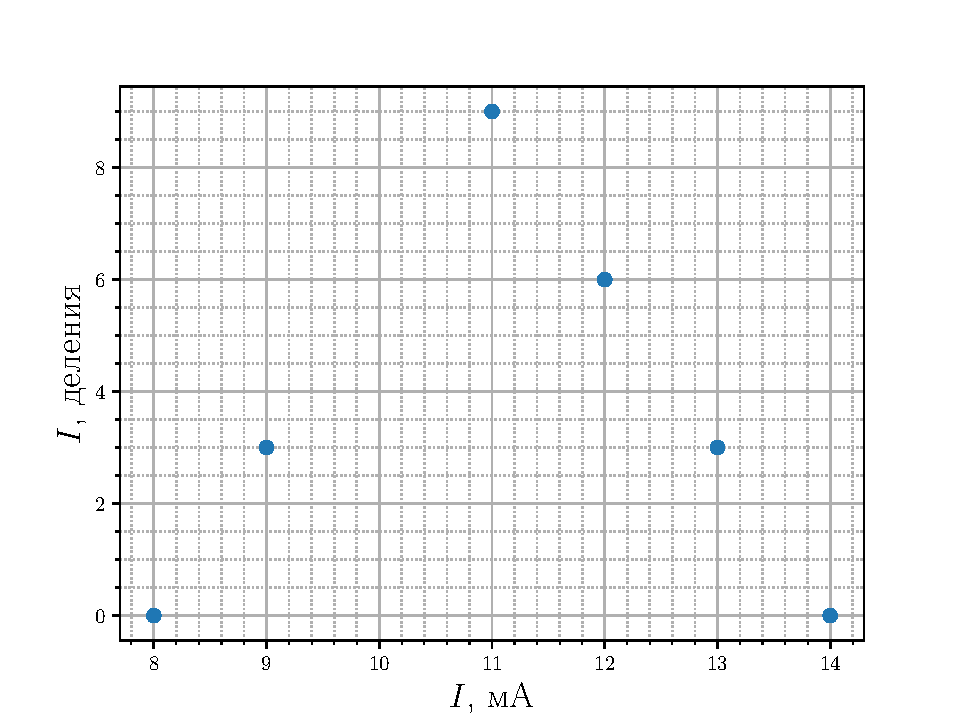
\includegraphics[height=0.4\textheight]{fig/res120Vref3V.pdf}
%     \caption{$U_{\text{рез}}=120$ В, $U_{\text{отр}}=3$ В}
%     \label{fig:res120Vref3V}
% \end{figure}
% \begin{figure}[H]
%     \centering
%     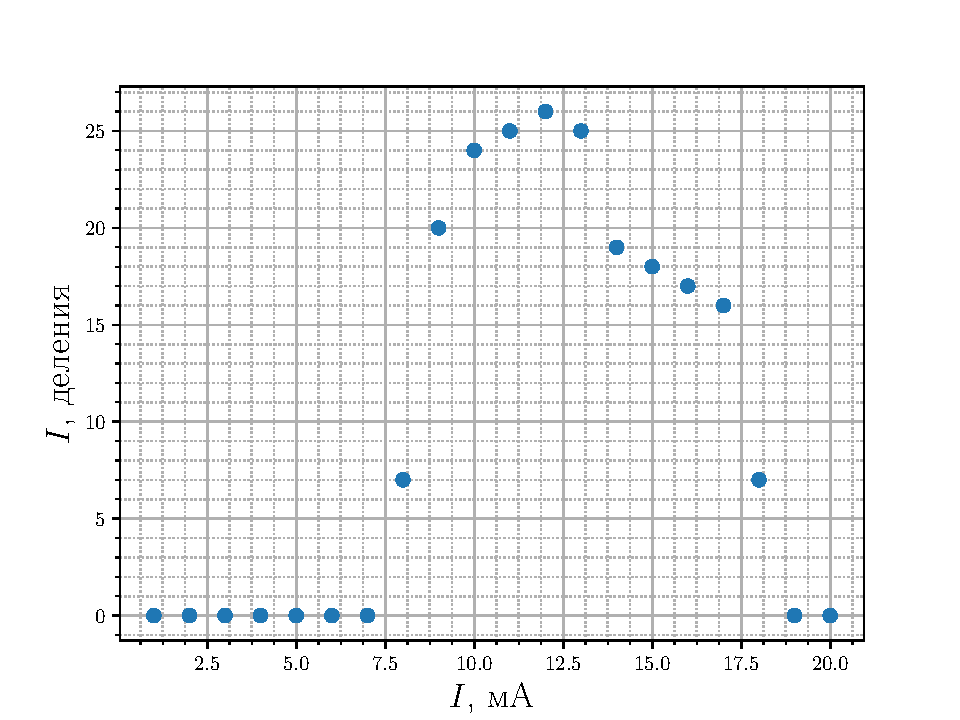
\includegraphics[height=0.4\textheight]{fig/res120Vref19V.pdf}
%     \caption{$U_{\text{рез}}=120$ В, $U_{\text{отр}}=19$ В}
%     \label{fig:res120Vref19V}
% \end{figure}
\begin{figure}[H]
    \centering
    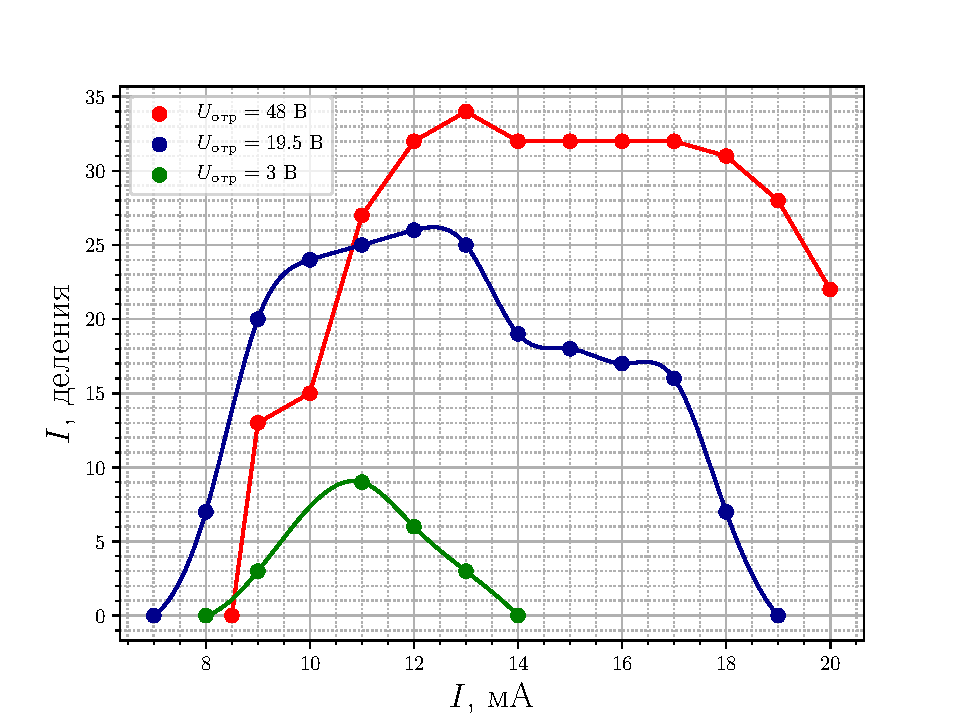
\includegraphics[height=0.4\textheight]{fig/task5}
    \caption{Зависимость тока в цепи детектора от тока пучка для трех различных зон генерации}
    \label{fig:task5}
\end{figure}

%\newpage

\section{Заключение}
В ходе работы было изучено устройство и основные принципы действия отражательного клистрона. Для математического описания использовалась теория тороидального резонатора, входящего в состав клистрона. Рассматривался процесс динамического управления плотностью в электронном пучке, возбуждение переменным конвекционным током пучка колебаний в резонаторе.  Рабочий режим соответствовал следующим напряжениям: 
\begin{itemize}
  \item $U_{\text{рез}}=96$ В
  \item $U_{\text{уск}}=126$ В
  \item $U_{\text{отр}}=42$ В
\end{itemize}

Получены зависимости тока в цепи детектора от напряжения на отражателе при постоянном напряжении на резонаторе и от напряжения на резонаторе при постоянном напряжении на отражателе. При помощи волномера измерена длина волны колебаний, создаваемых клистроном. А также, снята зависимость тока в цепи детектора от тока электронного пучка для трёх зон генератора. На основе экспериментальных данных были оценены ширина зазора в резонаторе и расстояние между резонатором и отражателем. Они получились равны соответственно 2 мм и 1 мм.
% \subsection{Контрольные вопросы}

% \begin{enumerate}
%   \item Объясните принцип работы отражательного клистрона.
%   \item Почему в приборах клистронного типа используются тороидальные ре­
%   зонаторы?
%   \item Можно ли для возвращения электронного потока в резонатор клистро­
%   на использовать не постоянное электрическое, а постоянное магнитное поле?
%   \item Что такое зоны генерации клистрона? Отличается ли структура поля
%   в резонаторе для центров различных зон генерации?
%   \item Как изменяется крутизна частотной перестройки клистрона с измене­
%   нием номера зоны и при вариации добротности резонатора?
% \end{enumerate}

\begin{thebibliography}{}
  \bibitem{litlink1}  Гапонов В.И. Электроника. 4.11. М.: Физматгиз, 1960-
  \bibitem{litlink2}  Лебедев И.В. Техника и приборы СВЧ. Ч.Н. М.: Высшая школа, 1972.
  \bibitem{litlink3}  Коетиенко А.И. Введение в электронику СВЧ. М.: Изд. МГУ, 1989.
  \bibitem{litlink4}  Градштейн И.С., Рыжик Н.М. Таблицы интегралов, сумм рядов и про­
  изведений. М., 1963. 5
  \bibitem{litlink5}  Вайнштейн Л.А. Электромагнитные волны. М.: Радио и связь, 1988.
\end{thebibliography}
\end{document}




\section*{Введение}
\addcontentsline{toc}{section}{Введение}
	Особенности движения носителей заряда в электрических и магнитных
полях определяют специфику функционирования подавляющего большинства
приборов современной микроэлектроники. Данное описание содержит краткое
изложение элементарных основ теории явлений переноса носителей заряда в 
однородном полупроводниковом материале. При этом речь пойдет как о движении
в электрических полях различной напряженности, однородно и неоднородно
распределенных в пространстве, так и о движении в скрещенных электрических
и магнитных полях, т.е. в условиях проявления эффекта Холла.

\section{Измерительная установка}

\begin{figure}[h!]
	\centering
	\includegraphics[width=\linewidth]{ris/3b.pdf}
	\vspace{-0.7em}
	\caption{Лабораторная установка}
	\label{fig:figure1}
\end{figure}

В состав лабораторной установки для исследования эффекта Холла входят (рис. \ref{fig:figure1}): 1 – источник питания образца, 2 – милливольтметр, 3 – согласующий модуль, 4 – исследуемый образец, 5 – электромагнит, 6 – источник питания электромагнита. На обзорном рисунке образец не изображен, он есть далее на рис. \ref{fig:hall} (стр. \pageref{fig:hall}).
\begin{enumerate}
\item Источник питания образца

Для питания образца используется источник питания GPS-3030D, включённый в режиме стабилизации напряжения. 

\item Милливольтметр 

Для измерения ЭДС Холла и балансировки схемы применён мультиметр APPA201N, работающий в режиме измерения постоянного напряжения на пределе 200 мВ. 

\item Согласующий модуль

Согласующий модуль обеспечивает соединение исследуемого образца, измерительных и питающих приборов в единую схему, согласование характеристик образца с параметрами источника питания, балансировку измерительной схемы.

\item Исследуемый образец

Исследуемый образец  -- полупроводниковая пластина, её размеры написаны на диамагнитном боксе, в который пластина помещена для обеспечения её экранировки, размещения в центре электромагнита, защиты от механических повреждений.
\item Электромагнит

Электромагнит создаёт постоянное магнитное поле. Конструктивно выполнен в виде катушки с обмоткой из медного провода, размещённой на Ш-образном ферромагнитном сердечнике. В центральном стержне сердечника выполнен зазор высотой 12 мм для размещения в нём образца. Максимальная напряжённость магнитного поля около 0,25 Тл. Величина магнитного поля зависит от тока, проходящего через обмотку. Расчётный коэффициент написан на электромагните.
\item Источник питания электромагнита

Для питания электромагнита используется такой же источник питания, как и у образца, но включённый в режиме стабилизации тока. 
\end{enumerate}

\subsection{Схема лабораторной установки}
Напряжение с источника питания GPS-3030D, работающего в режиме стабилизации напряжения, подаётся на образец через ограничительный резистор R1. Измерение тока образца производится стрелочным миллиамперметром, находящимся на передней панели согласующего модуля. Переключение пределов измерения миллиамперметра (10 мА – 3 мА) позволяет увеличить точность измерения тока образца. Сопротивление миллиамперметра при работе на пределе «3 мА» – 171 Ом, на пределе «10 мА» – 51 Ом. Для изменения направления тока через образец служит переключатель «Направление тока», имеющий среднее положение, в котором образец отключён от источника питания.
Для измерения ЭДС Холла используется мультиметр в режиме измерения постоянного напряжения на пределе 200 мВ. 
\begin{figure}[h!]
	\centering
	\includegraphics[scale=1.5]{ris/chem.pdf}
	\caption{Принципиальная схема включения (использовалось только направление $1\to2$)}
	\label{fig:figure2}
\end{figure}
Один из выводов мультиметра подсоединяется к контакту 3 образца, другой – к резистору R2 <<Балансировка>>.

\section{Теоретическая часть}


% \subsection{Движение носителей заряда в полупроводниках}
% Описание движения электрона в полупроводнике представляет собой достаточно сложную задачу, так как кроме внешних приложенных электрических и
% магнитных полей на электрон действует поля со стороны ионов, образующих
% кристаллическую решетку, и оставшихся электронов. Для того чтобы последующий материал был более доступен, мы последовательно рассмотрим движение
% электрона в идеальной кристаллической решетке, затем в решетке с дефектами и
% закончим данный раздел описанием движения ансамбля электронов в реальных
% полупроводниках.

% \subsubsection{Полуклассическая модель движения электронов в полупроводниках с идеальной кристаллической решеткой}

% Идеальная кристаллическая решетка представляет собой совокупность
% атомов, периодически (с периодом, равным периоду кристаллической решетки
% а) расположенных в пространстве. Потенциальная энергия электрона $V(\vec{r})$ в
% идеальной кристаллической решетке также является периодической функцией с
% периодом равным периоду кристаллической решетки: $V(\vec{r})=V(\vec{r} + \vec{a})$. Теорема
% Блоха утверждает, что собственные функции электрона, движущегося в таком
% периодическом поле, представляют собой модулированные плоские волны вида

% \begin{equation}
% 	\Psi_k (\vec{r})= e^{i(\vec{k}, \vec{r})} U_k(\vec{r}), 
% \end{equation}
% где $U_k(\vec{r})$ периодическая функция координат с периодом прямой решетки, $\vec{k}$
% - вектор, характеризующий квантовое состояние электрона в кристалле, имеющий размерность волнового вектора и поэтому названный квазиволновым вектором. Функции $\Psi_k(\vec{r})$ называют \textit{блоховскими функциями}. Можно ввести понятие квазиимпульса электрона с помощью соотношения соотношения $\vec{p} = \hbar \vec{k}$. При заданном значении $\vec{k}$ имеется много решений уравнений Шредингера, и описание энергетических уровней электрона в периодическом потенциале осуществляется посредством семейства непрерывных функций $\Psi_n(\vec{k})$ Совокупность всех электронных уровней, описываемых функцией $W_n(\vec{k})$ при фиксированном $n$, называют \textit{разрешенной энергетической зоной} с номером $n$. В дальнейшем номер разрешенном
% зоны $n$ будем опускать. Энергия электрона $W(\vec{r})$ в разрешенной зоне является
% периодической и четной функцией в пространстве обратной решетки \cite{lit1},\cite{lit2} , т.е.
% $W(\vec{k})= W(\vec{k} + \vec{G})$  (где $G$ -- вектор обратной решетки) и 
% $W(- \vec{k})=W(\vec{k})$. Заметим, что всегда можно рассматривать не бесконечное множество значений вектора $\vec{k}$, а ограничиться изменением компонент $\vec{k}$  в пределах зоны Бриллюэна, включающей в себя все физически неэквивалентные значения этого вектора.

% На уровне, заданном номером зоны п и квазиволновым вектором к электрон имеет отличную от нуля среднюю скорость
% \begin{equation}
% 	\vec{v} (\vec{k})= \frac{1}{\hbar} \nabla_{\vec{k}} W(\vec{k})
% \end{equation}

% Это очень интересный результат. Согласно ему электрон в периодическом потенциале имеет стационарные уровни, находясь на которых он, несмотря на
% взаимодействие с периодической последовательностью ионов, продолжает двигаться бесконечно долго, не теряя свое средней скорости.

% В общем случае состояние электрона описывается с помощью волнового
% пакета, состоящего и. блоховских функций. Если ширина пакета по квазиволновым векторам мала, по сравнению с зоной Бриллюэна и $W(\vec{k})$ мало меняется для
% уровней, входящих в волновой пакет, то скорость движения электрона есть ни
% что иное, как групповая скорость движения центра волнового пакета

% \begin{equation}
% 	\vec{v}_g(\vec{k})=\frac{1}{\hbar} \nabla_{\vec{k}} W(\vec{k})
% \end{equation}
% 	Если полупроводник находится во внешнем электрическом или магнитном поле
% то для описания изменения квазиволнового вектора $\vec{k}$ электрона и его координаты $\vec{r}$ можно воспользоваться полуклассической моделью. Она справедлива в
% случае, когда внешние электрические и магнитные поля медленно меняются в
% координатном пространстве на расстояниях порядка размера элементарной
% ячейки. Тогда при известной зависимости энергии электрона в разрешенной зоне
% $W(\vec{k})$ состояние электрона описывается его квазиволновым вектором $\vec{k}$, а также
% координатой $\vec{r}$. Считается, что в присутствии внешних электрических и магнитных полей $E$ и $B$

% \begin{enumerate}
% 	\item номер зоны электрона не меняется (т.е. в модели пренебрегается 
% 	возможностью межзонных переходов);
% 	\item изменения квазиволнового вектора и координаты электрона определяю icm
% уравнениями движения
% \end{enumerate}

% \begin{equation}
% 	\label{eq:1.4a}
% 	\dv{\vec{r}}{t}=\vec{v}_g (\vec{k})=\frac{1}{\hbar} \pdv{W(\vec{k})}{\vec{k}},
% \end{equation}
% \begin{equation}
% 	\label{eq:1.4b}
% 	\hbar \dv{\vec{k}}{t}= -e \qty(\vec{E}+ \qty[\vec{v}_g, \vec{B}] )
% \end{equation}

% Несмотря на сложность зависимости энергии электрона от квазиволнового
% вектора $W(\vec{k})$ в большинстве задач физики полупроводников играет роль поведение электрона в достаточно узкой области значений квазиволнового вектора в
% зоне Бриллюэна вблизи минимума или максимума энергии. Вблизи точки экстремума $\vec{k}_0$ функцию $W = W(\vec{k})$ можно разложить в ряд Тейлора, использую
% выражение
% \begin{equation}
% 	W(\vec{k})= W(\vec{k}_0)+\frac12 \sum_{i=x}^z \sum_{j=x}^z \frac{1}{m^*_{ij} }
% 	\hbar^2 (k_i-k_{i0})(k_j-k_{j0}),
% \end{equation}
% где $m_{ij}^*$ компоненты тензора \textit{эффективной массы} носителей зарядка, определяющиеся соотношением
% \begin{equation}
% 	\frac{1}{m^*_{ij}}=\frac{1}{\hbar^2} \pdv[2]{W(\vec{k})}{k_i}{k_j}\eval_{\vec{k}=\vec{k_0}}
% \end{equation}
% Выбрав соответствующую систему координат можно свести данный тензор к диагональному виду. В простейшем случае все компоненты тензора одинаковы, и тензор вырождается в скаляр, а закон дисперсии принимает параболическую форму
% \begin{equation}
% 	W(\vec{k})=W(\vec{k}_0) +\frac{1}{2m^*} \hbar^2 (\vec{k} - \vec{k} _0)
% \end{equation}
% Тогда уравнение движения электрона преобразуется к виду
% \begin{equation}
%  	\label{eq:electron_motion}
% 	m^* \vec{a} = -e \qty ( \vec{E}+ \qty[\vec{v}_g, \vec{B}] ),
% \end{equation}
% где $\vec{a}$ - ускорение электрона. Из формулы \eqref{eq:electron_motion} следует, что электрон в
% периодическом поле идеальной кристаллической решетки при воздействии
% внешнего электрического или магнитного поля ускоряется относительно решетки так, как если бы его масса была равна эффективной массе. Заметим, что
% эффективная масса электрона может принимать как положительные (около дна
% разрешенной зоны), так и отрицательные (около потолка разрешенной зоны)
% значений одной из самых впечатляющих особенностей зоной теории твердых тел
% является использование понятия дырок. Незанятые электронами (вакантные) со­
% стояния называют \textit{дырочными} состояниями или просто \textit{дырками}. Оказывается,
% что ток, получаемый при заполнении электронами совокупности определенного
% количества уровней в зоне, в точности совпадает с тем, который можно получить, если оставить эти уровни незаполненными и заполнить все остальные состояния в зоне частицами с положительным зарядом $+e$ (противоположным
% заряду электрона). Подчеркнем, что для одной и той же зоны нельзя пользоваться­ сразу двумя способами описания. Если считать, что ток переносят электроны, то незаполненные уровни не дают в него никакого вклада; если же считать, что ток переносят дырки, то отсутствует вклад от электронов Допустимо, однако, одни зоны описывать на языке электронов, а другие -- на языке дырок в зависимости от того, какой способ описания более удобен. Физические свойства дырки вытекают из факта заполненности электронами всех остальных состояний зоны.

% Они обобщены в \ref{tab:1} \cite{lit1}. Для более полного изучения свойств дырок рекомендуется обратиться к \cite{lit1} или \cite{lit2}.
% \begin{tabular}{c}
% 	\label{tab:1}
% \end{tabular}

% \subsubsection{Движение электронов  в реальных полупроводниках}

% Поле реальной кристаллической решетки не является строго периодическим из-за присутствия в полупроводнике дефектов Взаимодействие электрона с дополнительной силой, возникающей вследствие нарушения периодичности потенциала, приводит к рассеянию электрона, т.е. изменению электроном квазиволнового вектора и даже (в случае неупругого взаимодействия) энергии. В случае самой простой классификации дефекты кристаллической решетки можно от­нести к двум разным типам. Обычно рассматриваются так называемые \textit{статические} дефекты решетки, к которым относятся точечные дефекты, дислокации и т.д. и дефекты, \textit{перемещающиеся} по кристаллу.  К последним в первую очередь относятся тепловые колебания кристаллической решетки. Первый тип
% дефектов достаточно подробно был рассмотрен ранее (см. \cite{lit3}), здесь мы остановимся на особенностях второю типа дефектов кристаллическом решетки.

% \subsubsection{Колебания кристаллической решетки, фононы. Взаимодействие электронов с фононами}

% Известно, что атомы кристаллической решетки совершают хаотические
% колебания около положений устойчивого равновесия. Коллективное движение
% частиц в форме упругой волны называют нормальным колебанием кристаллической решётки. Зависимость частоты колебаний $\omega$ от волнового числа $q$ называют
% \textit{законом дисперсии} для колебаний атомов.

% В однородной струне как целом сплошном твёрдом теле могут возникать упругие волны, распространяющиеся со звуковой скоростью $v_\text{зв}$. При этом частота колебаний оказывается пропорциональной волновому числу: $\omega=q\cdot v_{\text{зв}}$.

% Абсолютная величина волнового числа может принимать значения от $0$ до $\infty$.

% Решение уравнения колебаний для линейной цепочки атомов одного сорта массой $M$ приводит к решению, соответствующему колебаниям с частотами
% \begin{equation}
% 	\omega=\pm \omega_{max} \sin{\frac{aq}{2}}.
% \end{equation}
% Здесь $\omega_{max}=2\sqrt{\frac{\beta}{M}}$, $a$--период решетки, $\beta$-- коэффициент квазиупругости, характеризующий взаимодействие между частицами при отклонении от положения равновесия. Скорость распространения упругой волны в этом случае зависит от длины волны $\lambda$, что является специфическим свойством упругих волн в среде с атомной структурой, отличающим последнюю от струны (или другого твёрдого тела) как сплошной среды. Имеем
% \begin{equation}
% 	v=\frac{\omega}{q}=\frac{\lambda}{\pi}\sqrt{\frac{\beta}{M}}\sin{\frac{\pi a}{\lambda}}
% \end{equation}
% Рассмотрим далее линейную цепочку атомов, в которой чередуются два
% типа частиц с массами $M_1$ и $M_2$ (рис. \ref{fig:1}). Расстояние между соседними атомами
% одного сорта по-прежнему равно $a$.

% Решение уравнения гармонических колебаний для такой системы будет содержать две ветви с частотами

% \begin{gather*}
% 	\omega_1^2=\frac{\omega_0^2}{2}\qty[1+\sqrt{1+ \gamma^2 \sin^2 \frac{aq}{2}	}] \\
% 	\omega_2^2=\frac{\omega_0^2}{2}\qty[1+\sqrt{1- \gamma^2 \sin^2 \frac{aq}{2}	}], 
% 	\text{ где} \\
% 	\omega_0^2=2 \beta \frac{M_1+M_2}{M_1M_2}, \gamma^2=4\frac{M_1M_2}{(M_1+M_2)^2} \\
% \end{gather*}
% \begin{figure}[h!]
% \begin{minipage}[h]{0.45\linewidth}
% 	\centering
% 	\includegraphics[width=\linewidth]{fig/11a}
% 	\caption{а) линейная цепочка с базисом из двух различных атомов}
% 	\label{fig:1.1a}
% \end{minipage}
% \hfill
% \begin{minipage}[h]{0.45\linewidth}
% 	\centering
% 	\includegraphics[width=\linewidth]{fig/11b}
% 	\caption{б) линейная цепочка с базисом из двух одинаковых атомов, при котором возникают оптические колебания}
% 	\label{fig:1.1b}
% \end{minipage}
% \vfill
% \begin{minipage}[h]{0.45\linewidth}
% 	\centering
% 	\includegraphics[width=\linewidth]{fig/11c}
% 	\caption{в) поперечные оптические колебания в линейной цепочке}
% 	\label{fig:1.1c}
% \end{minipage}
% \hfill
% \begin{minipage}[h]{0.45\linewidth}
% 	\centering
% 	\includegraphics[width=\linewidth]{fig/11d}
% 	\caption{акустические колебания}
% 	\label{fig:1.1d}
% \end{minipage}
% \end{figure}

% Колебания более высокой частоты $\omega_1$  принято называть \textit{оптическими}, а 
% с $\omega_2$-акустическими. При $q\rightarrow 0$ в оптической ветви колебаний атомы 
% решетки смещаются в противоположных направлениях, т.е. колеблются в противофазе, так что
% центр тяжести каждой пары, составляющей ячейку, остается неподвижным
% (рис. \ref{fig:1.1c}). В акустической же ветви атомы смещаются в одну сторону
% (рис. \ref{fig:1.1d}). На рис. \ref{fig:2} изображены соответствующие дисперсионные кривые колебаний.
% \begin{figure}[h!]
% 	\centering
% 	\includegraphics[width=0.5\linewidth]{fig/fig1_2}
% 	\caption{Дисперсионные кривые тепловых колебаний кристаллической решетки}
% 	\label{fig:2}
% \end{figure}

% Заметим, что выводы теории для линейной цепочки с чередующимися атомами разных масс в определенном смысле пригодны и для линейной цепочки с одинаковыми атомами, при условии, что имеются две подрешетки (рис. \ref{fig:1.1b}). В элементарной ячейке цепочки, изображенной на \ref{fig:1.1b} содержатся два атома. Оптические колебания возникают 
% в результате колебания в противофазе одной подрешётки  относительно другой. В объёмном кристалле сохраняются основные закономерности, справедливые для одномерной решетки. Поэтому оптические колебания наблюдаются, в частности, в $Si$ и $Ge$, которые сдержат один
% сорт атомов, но состоят из двух подрешеток (структура типа алмаза). Однако,
% для объемных кристаллов, имеющих в алиментарной ячейке только один атом,
% как и для простых (однородных) линейных цепочек, существуют только акустические колебания.

% Энергия каждого нормального колебания квантована. Нормальные колебания  можно рассматривать подобно линейным гармоническим осцилляторам с собственной частотой $\omega_{qj}$ и энергией
% \begin{equation}
% 	W_{qj}=\hbar \omega_{qj}\qty(n_{qj}+\frac12),
% \end{equation}
% где $n_{qj}=0,1,2,\dots$-- главное квантовое число $qj-$го осциллятора, колеблющегося с частотой
% $\omega_{qj}$, j - индекс ветви колебаний. 

% Полная энергия теплового движения атомов складывается из энергий всех нормальных колебаний
% \begin{equation}
% 	W=\sum_{q,j} W_{qj}=\sum_{q,j} \hbar \omega_{qj} (n_{qj}+\frac12),
% \end{equation}
% где волновое число $q$ имеет столько разрешенных значений, сколько в кристалле
% элементарных ячеек. При описании взаимодействия носителей заряда с тепловыми колебаниями решётки принято говорить о квазичастицах - фононах носителях квантов энергии колебаний решетки. При таком подходе изменение энергии колебаний решётки на один квант рассматривается как появление (или исчезновение) одного фонона с энергией и импульсом $ p = \hbar q$ . Процесс
% рассеяния электронов на тепловых колебаниях решетки теперь можно рассматривать как столкновение с фононом. При таком столкновении должны соблюдаться законы сохранения энергии и импульса 
% \begin{equation}
% 	\label{eq:lse}
% 	\vec{k}' = \vec{k} \pm \vec{q}, ~ W'= W\pm \hbar \omega_{qj},
% \end{equation}
% где $\vec{k}$, $\vec{q}$ - волновые векторы электрона и фонона до столкновения; $\vec{k}'$ - волновой вектор электрона после столкновения; $W$ и $W'$ - соответственно, энергия электронов до и после столкновения. Процесс, соответствующий в \eqref{eq:lse} знаку плюс, интерпретируется как поглощение, а знаку минус -- испускание электроном фонона.

% В некоторых отношениях фононы ведут себя не так, как обычные частицы. Во-первых, среднее число фононов зависит от температуры, а во-вторых, при взаимодействии, например, с электронами или друг с другом фононы возникают и исчезают. Поэтому их называют квазичастицами.

% \subsubsection{Дрейф электрона во внешнем электрическом поле}


% Рассмотрим движение электрона в реальном полупроводнике во внешнем электрическом поле. Так как в реальной кристаллической структуре присутствуют дефекты частица движется ускоренно лишь на небольшом участке пути, а затем испытывает рассеяние, теряет направленную скорость, псле чего процесс разгона начинается заново. Движение электрона между актами рассеяния по прежнему описывается уравнениями  \eqref{eq:1.4a} и \eqref{eq:1.4b}. Если время свободного пробега электрона (время между двумя процессами рассеяния) мало по сравнению со временем движения электрона от одного края зоны Бриллюэна до другого, то эффективная масса электрона мало меняется во время его свободного пробега. Тогда зависимость проекции мгновенной скорости электрона на ось, направленную против внешнего электрического поля представлена на рис. \ref{fig:3}. Линейный участок на графике соответствует ускорению электрона во внешнем поле, вертикальный -- рассеянию электрона. Благодаря наличию внешнего поля электрон обладает средней скоростью направленного движения вдоль поля, которая называется \textit{дрейфовой скоростью}.

% В слабых электрических полях дрейфовая скорость пропорциональна напряженности электрического поля:
% \begin{equation}
% \label{eq:1.14}
% 	v=\mu E
% \end{equation}

% \begin{figure}[h!]
% 	\centering
% 	\includegraphics[width=0.5\linewidth]{fig/13}
% 	\caption{Зависимость проекции мгновенной скорости носителей заряда от времени}
% 	\label{fig:3}
% \end{figure}

% Коэффициент пропорциональности между скоростью и полем $\mu$ называется подвижностью носителей заряда . Эта величина численно равна средней скорости
% направленного движения частиц в электрическом поле с единичной напряженностью.

% Интересно, что при увеличении электрического поля дрейфовая скорость
% перестает расти по линейному закону и в больших полях или стремится к установившемуся значению или уменьшается. Типичные зависимости скорости
% дрейфа носителей заряда в различных полупроводниках приведены на рис.\ref{fig:4}

% \begin{figure}[h!]
% 	\centering
% 	\includegraphics[width=0.5\linewidth]{fig/14}
% 	\caption{Экспериментальные зависимости дрейфовой скорости носителей зарада от напряженности электрического поля для $Ge$, $Si$, $GaAs$}
% 	\label{fig:4}
% \end{figure}

% Характер зависимости $v(E)$ определяется как структурой зоны проводимости полупроводника, так и механизмами рассеяния. В валентных материалах основной причиной ограничения дрейфовой скорости является рассеяние на оптических фононах. В отличие от почти упругого рассеяния на акустических фононах, рассеяние на оптических фононах является резко неупругим, т. е. про­
% исходит существенное изменение энергии носителей заряда. Как только энергия
% электрона становится выше энергии оптического фонона (см. рис. \ref{fig:2}), резко
% возрастает количество актов столкновений, сопровождающихся возбуждением
% фонона. Таким образом, электрон активно отдаёт энергию кристаллической
% решетке, что препятствует дальнейшему росту скорости его направленного движения. В режиме насыщения скорости вся энергия, набираемая электроном в электрическом поле за время свободного пробега, отдаётся им в кристаллическую решётку посредством возбуждения фононов.

% В полупроводниковых соединениях ($GaAs$, $InP$ и др.) на зависимость сред­ней скорости электронов от напряженности электрического поля существенно влияет переход электронов из $\Gamma$-долины с низкой эффективной массой носителей
% заряда в верхние $L$ и $X$ долины со значительно большей массой и меньшей подвижностью (средней дрейфовой скоростью) электронов \cite{lit4}-\cite{lit5}. Как правило, такой
% процесс происходит при столкновении с оптическим фононом. После столкновения направленная скорость электрона в среднем теряется. В результате этих
% процессов на зависимости средней скорости электронов от напряженности электрического поля появляется экстремум, а количество электронов, находящихся в
% верхних долинах, (заселенность долин) растет с увеличением напряженности по­
% ля.

% \subsubsection{Движение носителей зарядка в плавно изменяющихся во времени или в пространстве электрических полях}


% Наиболее общей системой уравнений, описывающей перемещение во
% внешнем электрическом поле ансамбля электрически заряженных частиц в случае, когда электрические поля медленно меняются во времени\footnote{по сравнению со временем релаксации энергии электронов $\tau_W$} или в пространстве\footnote{по сравнению с длиной релаксации энергии электронов $l_W=\tau_W\cdot v_T$, где $v_T$-- тепловая скорость электрона при температуре T}, является система уравнений, включающая в себя

% \begin{itemize}
% 	\item \textbf{уравнение Пуассона} (полученное из предположения о малости скорости дрейфа носителей заряда в полупроводниковом материале по сравнению со скоростью света, когда справедливо выражение $\vec{E}=-\nabla \varphi $)
% \begin{equation}
% 	\label{eq:1.15}
% 	\Delta \varphi =- \frac{1}{\epsilon \epsilon_0} \rho(x,y,z),
% \end{equation}
%  где $\vec{E}$ - напряженность электрического поля, $\varphi$- потенциал, $\epsilon$-диэлектрическая проницаемость материала, $\rho(x,y,z)$- объемная плотность зарядка (включает в себя подвижные заряды электронов и дырок, а также неподвижные заряженные структурные дефекты полупроводника, в том числе, ионизированные примеси);

%  	\item \textbf{выражения для плотности электронного и дырочного токов}

%  	\begin{gather}
%  		\vec{j}_n = -en \vec{v}_n + e\cdot \nabla(D_n n) \\ 
%  		\label{eq:1.16a}
%  		\vec{j}_p = ep \vec{v}_p - e\cdot \nabla(D_p p), \\
%  		\label{eq:1.16b}
%  	\end{gather}
%  	n,p - концентрации, а $\vec{v}_n$ $\vec{v}_p$ - дрейфовые скорости электронов и дырок, соответственно; $e$- абсолютная величина заряда электрона; $D_n$, $D_p$- коэффициенты диффузии носителей заряда; каждое из выражений \eqref{eq:1.16b} и \eqref{eq:1.16a} для плотности тока содержит \textit{дрейфовую} (которая определяется движением носителей в электрическом поле) и \textit{диффузионную} (которая возникает из-за теплового движения подвижных зарядов) составляющие.

%  	\item \textbf{уравнения непрерывности для электронов и дырок}, которые в отсутствие генерации и рекомбинации частиц записываются в виде
%  	\begin{equation}
%  		\label{eq:1.17}
%  		\pdv{n}{t}=\frac{1}{e}\div{\vec{j}_n}, ~ \pdv{p}{t}=-\frac{1}{e}\div{\vec{j}_p}
%  	\end{equation}

% \end{itemize}
%  	Система уравнений \eqref{eq:1.15}-\eqref{eq:1.17} дополняется \textit{соотношением Эйнштейна}, описывающим связь между подвижность и коэффициентом диффузии
%  	\begin{equation}
%  		D=\frac{kT}{e}\mu
%  	\end{equation}
%  	и выражением для дрейфовой скорости носителей зарядка как функции электрического поля
%  	\begin{equation}
%  		v_n=v_n(E) \text{ и } v_p=v_p(E)
%  	\end{equation}
%  	Тогда выражение для полной плотности тока в полупроводнике записывается в виде
%  	\begin{equation}
%  		\vec{j} = \vec{j}_n +\vec{j}_p +\pdv{E}{t},
%  	\end{equation}
%  	где третье слагаемое описывает ток смещения.


%  	\subsubsection{Движение носителей заряда в резко изменяющихся во времени или пространстве электрических полях}


% Для описания движения носителей заряда в полупроводниковых структурах при резко изменяющихся полях используется система уравнений, которая,
% помимо уравнений \eqref{eq:1.15} - \eqref{eq:1.17} включает в себя уравнение баланса импульса
% \eqref{eq:1.23}, уравнение баланса энергии \eqref{eq:1.24} и выражение для плотности потока
% энергии \eqref{eq:1.26}. В случае транспорта электронов полная система уравнений имеет
% следующий вид:
% \begin{gather}
% 	\label{eq:1.21}
% 	\Delta  \varphi = -\frac{e}{\epsilon \epsilon_0} \qty(N_d-n)  \\
% 	\label{eq:1.22}
% 	\pdv{n}{t}=\frac{1}{e} \div{\vec{j}_n}\\
% 	\label{eq:1.23}
% 	\dv{ \qty (m^*\vec{v}) }{t}= -e\vec{E} - \frac{m^*}{\tau_p} \vec{v} \\
% 	\label{eq:1.24}
% 	\pdv{(Wn)}{t}=\div{\vec{j}_W}+ \qty(\vec{j}_n, \vec{E})-\frac{n\qty(W-W_0)}{\tau_W} \\
% 	\label{eq:1.25}
% 	\vec{j}_n = - en\vec{v} + e\cdot \grad{(D_n n)} \\
% 	\label{eq:1.26}
% 	\vec{j}_W= -nW \vec{v} +\grad{(D_n n W)} \\ 
% 	\label{eq:1.27}
% 	\vec{j} = \vec{j}_n + \pdv{\vec{E}}{t} \\
% 	\label{eq:1.28} 
% 	\vec{E}=-\grad{\varphi}
% \end{gather}
% Здесь $N_d$ - концентрация доноров; 
% $m^*$- эффективная масса электронов;
% $\vec{j}_W$- плотность потока энергии электронов;
% $\tau_p, \tau_W$- \textit{времена релаксации} импульса и энергии носителей;
% $W_0=\frac32 kT$- средняя тепловая энергия электронов.

% Уравнения баланса \eqref{eq:1.26} и \eqref{eq:1.24} выражают, по сути, законы сохранения
% импульса и энергии частиц. Импульс направленного движения электронов может
% увеличиваться за счет разгона в электрическом поле (первое слагаемое в правой
% части \eqref{eq:1.23} и уменьшаться из-за рассеяния носителей на дефектах структуры
% (второе слагаемое). Энергия носителей в некотором замкнутом объеме, помимо
% тех же причин, может изменяться за счет втекания или вытекания горячих (т е.,
% высокоэнергетических) или холодных носителей, что отражает первое слагаемое
% в правой части \eqref{eq:1.24}.
% В стационарном состоянии $\dv{(m^*v)}{t}=0, ~ \pdv{W}{t}=0$ уравнения \eqref{eq:1.23} и
% \eqref{eq:1.24} принимают следующий вид:
% \begin{gather}
% 	\label{eq:1.29}
% 	\tau_p=\frac{m^*v_s}{eE} \\
% \label{eq:1.30}
% 	\tau_W=\frac{W_s-W_0}{eEv_s},
% \end{gather}

% где индекс <<s>> означает стационарное значение. Выражения \eqref{eq:1.29}, \eqref{eq:1.30}
% связывают времена релаксации со стационарными значениями скорости и энергии.
% Время релаксации по импульсу, как правило, много меньше времени релаксации
% по энергии, т.к. упругие столкновения не изменяют энергию, но могут существенно изменить импульс частицы. На рис. \ref{fig:5} приведены графики зависимости
% времени релаксации энергии и импульса в кристаллах $Si$ и $GaAs$ от величины
% средней энергии носителей заряда.
% \begin{figure}[h!]
% 	\centering
% 	\includegraphics[width=0.7\linewidth]{fig/15}
% 	\caption{Зависимость времени релаксации энергии и импульса от разницы между средней 
% 	($W$) и тепловой энергией ($W_0$) электронов в кристаллах $Si$ и $GaAs$}
% 	\label{fig:5}
% \end{figure}
% Из \eqref{eq:1.14} и \eqref{eq:1.29} следует, что 
% \begin{equation}
% \label{eq:1.31}
% 	\mu =\frac{e \tau_p}{m^*}
% \end{equation}
% Даже в случае полупроводников с высокой подвижностью носителей заряда,
% максимальная стационарная дрейфовая скорость частиц не превышает I-
% $3\cdot 10^7\frac{\text{см}}{\text{с}}$, что, казалось бы, накладывает принципиальное ограничение на быстродействие твердотельных приборов. Однако в динамическом режиме и в коротких образцах можно получить дальнейшее увеличение дрейфовой скорости электронов. Суть этого явления состоит в следующем. Когда носители попадают в
% область резкого скачка поля, скорость направленного движения начинает быстро
% расти у всех частиц одновременно. Поэтому средняя скорость носителей заряда в
% течение короткого периода времени может быть существенно выше ее стационарного значения (\textit{эффект всплеска скорости во времени}). Затем столкновения электронов с дефектами структуры приводят к сбросу средней скорости частиц и через некоторое время (порядка нескольких времен релаксации импульса) устанавливается стационарное значение средней по ансамблю скорости носителей для данного значения поля. Таким образом, если не <<дожидаться>>
% установления стационарной скорости, а использовать нестационарное значительное увеличение дрейфовой скорости частиц на временах $\sim \tau_p$, то можно получить значительное увеличение дрейфовой скорости частиц, что существенно сказывается на параметрах полупроводниковых приборов. На рис. \ref{fig:6} приведены расчетные зависимости $v(t)$ для 
% $GaInAs$\footnote{$GaInAs$ -- тройное полупроводниковое соединение, отличающиеся от $GaAs$ тем, что часть атомов галлия замещена индием}, $InP$  и $GaAs$.
% \begin{figure}[h!]
% 	\centering
% 	\includegraphics[width=0.7\linewidth]{fig/16}
% 	\caption{Изменение дрейфовой скорости электронов во времени после мгновенного включения электрического поля $E=40$ кВ/см. Кривые и точки соответствуют различным методам счета \cite{lit6}}
% 	\label{fig:6}
% \end{figure}

% Характерные размеры активной области современных диодов и транзисторов имеют значения порядка 10-100 нм. В таких условиях длина прибора может стать сравнимой со средней длиной свободного пробега носителей в полупроводнике, а время пролета может оказаться примерно равным или меньше среднего времени релаксации энергии и импульса носителей заряда. В таких условиях равновесное распределение носителей не успевает установиться, и средняя дрейфовая скорость электронов во всей активной области прибора может существенно превосходить значения насыщенной скорости в длинных образцах. Это увеличение скорости за счет нестационарных эффектов получило название \textit{эффект всплеска скорости в пространстве}. На рис. \ref{fig:7} приведены рассчитанные максимальные значения дрейфовой скорости для коротких образцов $GaAs$. Как видим, даже у образцов 300-500 нм величина скорости остается много больше максимального стационарного значения $v_s \approx 3\cdot 10^7$ см/с.
% \begin{figure}[h!]
% 	\centering
% 	\includegraphics[width=0.7\linewidth]{fig/17}
% 	\caption{Зависимости максимального значения средней дрейфовой скорости в образцах с различной длиной l, рассчитанные для $GaAs$ при двух значениях концентрации примеси: 1- $N_d=0$; 2 - $N_d=3\cdot 10^{17} \text{см}^{-3}$. $T=293 K$}
% 	\label{fig:7}
% \end{figure}

% В многодолинных полупроводниках, как и в стационарном случае, на динамику дрейфовой скорости на коротких отрезках времени существенно влияет междолинного переброса. Если в многодолинных материалах эффект всплеска скорости обычно сопровождается переходом в верхние долины, то в полупроводниках типа $Si$ и $Ge$ всплеск скорости не так явно выражен, но тем не менее, увеличение скорости может составлять 1.5-3 раза.

\subsection{Элементарная теория эффекта Холла}
Анализ транспорта носителей в полупроводниковых структурах, представленный в предыдущем разделе, требует знания концентрации носителей заряда и их подвижности в материале. Эти характеристики являются важными физическими величинами, определяющими многие свойства полупроводников, например, электропроводность, теплопроводность, термо-ЭДС и др.

Концентрацию и подвижность в отдельности можно определить, зная соотношение между ними. В данной работе это соотношение устанавливается экспериментально при помощи эффекта Холла.

Эффект Холла представляет собой поперечный гальваномагнитный эффект, суть которого заключается в следующем: если поместить полупроводниковую пластину во внешнее магнитное поле $\vec{B}$ (рис. \ref{fig:8}) и пропустить вдоль нее ток, то вследствие смещения движущихся зарядов к одной из граней пластины возникает поперечная разность потенциалов, называемая \textit{ЭДС Холла}. При этом (см. рис. \ref{fig:8}.б, \ref{fig:8}.в), носители различных знаков смещаются к одной и той же боковой грани полупроводника, поэтому с изменением типа электропроводности меняется и знак ЭДС.

С помощью эффекта Холла можно экспериментально определить тип носителей, концентрацию и подвижность в данном полупроводниковом образце. Другим важным практическим приложением этого эффекта являются измерения силы тока и мощности в цепях постоянного и переменного тока  (вплоть до очень высоких частот), напряженности постоянных и переменных магнитных полей, преобразование сигналов, анализ спектров и т.д.

\begin{figure}[h!]
\begin{minipage}[h]{0.329\linewidth}
		\centering
	\includegraphics[width=\linewidth]{fig/21a}
\end{minipage}
\begin{minipage}[h]{0.329\linewidth}
		\centering
	\includegraphics[width=\linewidth]{fig/21b}
\end{minipage}
\begin{minipage}[h]{0.329\linewidth}
		\centering
	\includegraphics[width=\linewidth]{fig/21c}
\end{minipage}
	\caption{Возникновение ЭДС Холла: схема эксперимента (а); смещение носителей заряда в дырочном (б) и электронном (в) полупроводниках, соответственно}
	\label{fig:8}
\end{figure}

Разберем эффект Холла более подробно. На рис. \ref{fig:8}.а показан полупроводник, две плоскости которого подключены через омические (т.е. невыпрямляющие) контакты к внешней батарее. Обозначим $\vec{j}$ плотность тока в направлении Ox. Магнитное поле $\vec{B}$ приложено в направлении Oy. Рассмотрим электрон, двигающийся в отрицательном направлении оси Ox со средней скоростью $\vec{V}$. На движущийся в магнитном поле электрон действует магнитная составляющая силы Лоренца:
$$\vec{F} = -e [\vec{v}, \vec{B}].$$
В результате действия этой силы траектория электрона будет искривляться  в направлении оси z, и, поскольку в этом направлении ток протекать не может, электроны будут накапливаться на боковой поверхности ($z=\pm a$, см. рис. \ref{fig:8}) до тех пор, пока не установится электрическое поле $\vec{E}_H$, достаточное для создания силы. равной магнитной составляющей силы Лоренца, но направленной противоположно. Приравнивая эти силы, получим: 
\begin{equation}
\label{eq:2.1}
	\vec{E}_H=[\vec{v}, \vec{B}]
\end{equation}

Воспользуемся законом Ома в дифференциальной форме:
\begin{equation}
\label{eq:2.2}
	\vec{j} = \sigma \vec{E},
\end{equation}
где $\sigma = e \cdot n \cdot \mu_n$ - удельная проводимость образца, $\mu_n = \frac{v}{E}$ - подвижность носителей. Соотношение \eqref{eq:2.2} перепишем в следующем виде:
\begin{equation}
\label{eq:2.3}
	\vec{j} = e \cdot n \cdot \mu_n \cdot \vec{E} = -e \cdot n \cdot \vec{v}
\end{equation}

Исключая $v$ из соотношения \eqref{eq:2.1}, получим:
\begin{equation}
\label{eq:2.4}
	\vec{E}_H = -\frac{1}{en} [\vec{j}, \vec{B}]=R[\vec{j}, \vec{B}]
\end{equation}

Учитывая, что полный ток через образец $I=jab$, а поперечная ЭДС $U_H=E_Ha$, получим соотношение, связывающее ЭДС Холла с величиной электрического тока:
\begin{equation}
\label{eq:2.5}
	U_H=R \cdot \frac{I\cdot B}{b}
\end{equation}

Величина R называется \textit{постоянной Холла} и определяется как

\begin{equation}
\label{eq:2.6}
	R=-\frac{1}{e\cdot n}
\end{equation}

Поперечную ЭДС $U_H$, ток I, напряженность магнитного поля B (для немагнитных образцов) и толщину b полупроводникового образца можно измерить. Это позволяет найти численное значение постоянной Холла.

В действительности, произведенный элементарный вывод коэффициента Холла \eqref{eq:2.6} неточен: в нем не учтена разница между мгновенной скоростью электронов, входящей в выражение магнитной составляющей силы Лоренца, и дрейфовой скоростью, которую электрон приобретает под действием электрического поля. Кроме того, не учитывается распределение электронов по скоростям и механизмы рассеяния носителей. Формула \eqref{eq:2.6} оказывается справедливой только для металлов и вырожденных полупроводников (вырожденным называется полупроводник с очень высокой, порядка $10^{19}$ атом/$\text{см}^3$, концентрацией примеси). Более строгий анализ дает для невырожденных полупроводников значение R, которое отличается от выражения \eqref{eq:2.6} множителем А. Если учитывать рассеяние носителей только на кристаллической решетке (взаимодействие с фононами), то $A=\frac{3\pi}{8}$. В общем виде постоянная Холла может быть записана как:
\begin{gather}
	R=-\frac{A}{n\cdot e} \text{(для полупроводника n-типа)} \notag \\
	R=\frac{A}{p\cdot e} \text{(для полупроводника p-типа)}
\label{eq:2.7}
\end{gather}
где множитель А может принимать значения от 1 до 1.7. Знак минус в формуле \eqref{eq:2.7} демонстрирует, что ЭДС Холла для электронного полупроводника имеет полярность, противоположную полярности для дырочного полупроводника.

Знание электропроводности и постоянной Холла позволяет найти как концентрацию носителей, так и их подвижность.

Обозначим через холловский угол $\theta_H$ малый угол, который образует с осью х вектор напряженности суммарного электрического поля (см. рис. \ref{fig:8}):
\begin{equation}
\label{eq:2.8}
	\theta_H \cong \tg{\theta_H}=\frac{E_H}{E}
\end{equation}


Из \eqref{eq:2.8} с учетом \eqref{eq:2.2} и \eqref{eq:2.4} получим:
\begin{equation}
\label{eq:2.9}
	\theta_H = \mu_{nH} \cdot B
\end{equation}
где $\theta_H$-холловский угол в проводнике n-типа, а $\mu_{nH}$ - так называемая \textit{холловская подвижность} электронов (индекс H указывает на метод определения подвижности). Численное значение холловской подвижности может расходиться с величиной подвижности, определенной другими методами (например, прямым способом, основанным на измерении времени распространения носителей тока по полупроводнику на определенное расстояние с известным ускоряющим полем). Последняя называется дрейфовой подвижностью. Дрейфовую подвижность можно определить из выражения \eqref{eq:2.4}, если, используя выражение \eqref{eq:2.7}, преобразовать его к виду:
\begin{equation}
\label{eq:2.10}
	\vec{E}_H = -\frac{A}{en}\cdot\dotvec[j,B]=-A\cdot \mu_{nd} \cdot [\vec{E},\vec{B}],
\end{equation}
где индекс d при $\mu_{nd}$ указывает, что это дрейфовая подвижность электронов.

Из выражений \eqref{eq:2.8}-\eqref{eq:2.10} следует, что для электронов $\mu_{nH}=A\cdot \mu_{nd}$, а для дырок $\mu_{pH}=A\cdot \mu_{pd}$. Используя выражения \eqref{eq:2.2} и \eqref{eq:2.7}, получим:
\begin{equation}
\label{eq:2.11}
	\mu_{(n,p)H}=R\cdot \sigma.
\end{equation}

Приведенные выше выражения относились к полупроводникам, у которых концентрация неосновных носителей пренебрежимо мала по сравнению с концентрацией основных (униполярная проводимость). Расчет постоянной Холла для материала со смешанной проводимостью приводит к формуле:
\begin{equation}
\label{eq:2.12}
	R= \frac{A}{e}\cdot \frac{n\mu^2_{nd}-p\mu^2_{pd}}{(n\mu_{nd}+p\mu_{pd})^2}.
\end{equation}
для собственного полупроводника $(n=p=n_i)$ получим:
\begin{equation}
\label{eq:2.12}
	R= \frac{A}{e}\cdot \frac{\mu^2_{nd}-\mu^2_{pd}}{\mu_{nd}+\mu_{pd})}\cdot \frac{1}{n_i}.
\end{equation}

% У собственных полупроводников R обычно отрицательна, т.к. подвижность электронов чаще всего больше подвижности дырок. На рис. \ref{fig:9} показаны зависимости подвижности электронов и дырок от концентрации примесей в наиболее распространенных полупроводниках.

% \begin{figure}[h!]
% 	\centering
% 	\includegraphics[width=0.7\linewidth]{fig/22}
% 	\caption{Зависимость дрейфовой подвижности электронов и дырок в $Si$ и $Ge$ и холловской подвижности в $GaAs$ от концентрации атомов легирующей примеси (T=300 K)}
% 	\label{fig:9}
% \end{figure}

% 
% \subsection{Измерительная установка и методика измерений}

% В данной работе измерение постоянной Холла производится на переменном токе (см. блок-схему на рис.\ref{fig:10}). Этот метод дает возможность предельно упростить схему, т.к. использование переменного тока позволяет применять в качестве индикаторов ЭДС Холла широко распространенные измерительные приборы (ламповые вольтметры, осциллографы и др., имеющие достаточно большое входное сопротивление) вместо обычно используемых схем компенсации. Кроме того, при работе на переменном токе легко устраняется паразитная разность потенциалов, которая возникает между холловскими контактами вследствие их несимметричного расположения.

% Схема работает следующим образом: переменное напряжение подается со звукового генератора I через трансформатор Тр, регулировочный потенциометр $R1$, который выведен на переднюю панель установки (на лабораторной установке - ручка "ток образца") и миллиамперметр II подается на образец. Величина тока через образец устанавливается потенциометром $R1$. На одной из боковых поверхностей образца вместо одного холловского контакта установлены два (4,5), потенциал одного из которых заведомо выше, а другого заведомо ниже потенциала 3, расположенного на противоположной поверхности. Потенциометр $R3$ легко позволяет найти точку с потенциалом, равным потенциалу контакта 3, т.е. произвести балансировку холловских контактов. Для этого оправку с образцом устанавливают на опорную площадку вне магнитного поля и, установив ток через образец в пределах 5-6 мА, вращением ручки потенциометра $R3$ (он расположен на оправке) добиваются минимального отклонения луча осциллографа, подключенного вертикальным усилителем к выходному разъему IV установки (усилитель при этом выводится на предельное усиление). После проведения балансировки по осциллографу производится ее проверка на милливольтметре. Балансировка считается удовлетворительной, если сигнал на милливольтметре не превышает 0.5 мВ. 
% \begin{figure}[h!]
% 	\centering
% 	\includegraphics[width=\linewidth]{example-image-a}
% 	\caption{Блок-схема измерительной установки}
% 	\label{fig:10}
% \end{figure}

% % После этой проверки оправка с образцом переносится в зазор с магнитным полем и фиксируется на нижнем полюсном наконечнике. При этом надо избегать резких ударов и толчков, т.к. можно сбить балансировку. Выходной разъем V установки служит в качестве источника сигнала, имеющего ту же фазу, что и напряжение на контакте 2 относительно контакта 1. Это опорное напряжение необходимо при определении типа носителей в данном образце. Для определения типа носителей сигнал с выхода IV подается на вертикальный усилитель, а с выхода V - на горизонтальный (при этом ручка осциллографа <<диапазон частот>> должна находится в положении <<выкл.>>). Установив ток через образец 5-7 мА, а усилители осциллографа в режим усиления, наиболее удобный для наблюдения, легко определить разность фаз между контактами 2 и 3 относительно <<земли>>, по которой, зная направление магнитного поля, можно установить тип носителей. Величина магнитного поля может меняться путем изменения расстояния между полюсными наконечниками. 
% \subsection{Измерительная установка}

% В состав лабораторной установки для исследования эффекта Холла входят (\ref ): 1 – источник питания образца, 2 – милливольтметр, 3 – согласующий модуль, 4 – исследуемый образец, 5 – электромагнит, 6 – источник питания электромагнита, 7 – соединительные провода.
% \begin{enumerate}
% \item Источник питания образца

% Для питания образца используется источник питания GPS-3030D, включённый в режиме стабилизации напряжения. 

% \item Милливольтметр 

% Для измерения ЭДС Холла и балансировки схемы применён мультиметр APPA201N, работающий в режиме измерения постоянного напряжения на пределе 200 мВ. 

% \item Согласующий модуль

% Согласующий модуль обеспечивает соединение исследуемого образца, измерительных и питающих приборов в единую схему, согласование характеристик образца с параметрами источника питания, балансировку измерительной схемы.

% \item Исследуемый образец

% Исследуемый образец (рис. 3.3 а, 3.3 б) – полупроводниковая пластина, её размеры написаны на диамагнитном боксе, в который пластина помещена для обеспечения её экранировки, размещения в центре электромагнита, защиты от механических повреждений.
% \item Электромагнит

% Электромагнит создаёт постоянное магнитное поле. Конструктивно выполнен в виде катушки с обмоткой из медного провода, размещённой на Ш-образном ферромагнитном сердечнике. В центральном стержне сердечника выполнен зазор высотой 12 мм для размещения в нём образца. Максимальная напряжённость магнитного поля около 0,25 Тл. Величина магнитного поля зависит от тока, проходящего через обмотку. Расчётный коэффициент написан на электромагните.
% \item Источник питания электромагнита

% Для питания электромагнита используется источник питания GPS-3030D, включённый в режиме стабилизации тока. 
% \end{enumerate}
 
\subsection*{Описание работы установки}
Напряжение с источника питания GPS-3030D, работающего в режиме стабилизации напряжения, подаётся на образец через ограничительный резистор R1. Измерение тока образца производится стрелочным миллиамперметром, находящимся на передней панели согласующего модуля. Переключение пределов измерения миллиамперметра (10 мА – 3 мА) позволяет увеличить точность измерения тока образца. Сопротивление миллиамперметра при работе на пределе «3 мА» – 171 Ом, на пределе «10 мА» – 51 Ом. Для изменения направления тока через образец служит переключатель «Направление тока», имеющий среднее положение, в котором образец отключён от источника питания.
Для измерения ЭДС Холла используется мультиметр в режиме измерения постоянного напряжения на пределе 200 мВ. Один из выводов мультиметра подсоединяется к контакту 3 образца, другой – к резистору R2 «Балансировка». Необходимость балансировки обусловлена тем, что при подсоединении измерительных контактов к образцу невозможно их расположить абсолютно точно друг напротив друга, в результате чего между этими выводами появится паразитная разность потенциалов, обусловленная током образца, которая будет давать систематическую ошибку измерения ЭДС Холла. Чтобы её уменьшить, с одной из сторон делаются два контакта (4 и 5), к которым подсоединяются крайние выводы переменного резистора R2. Изменяя положение движка резистора R2, можно найти точку с потенциалом, равным потенциалу контакта 3. При этом показания мультиметра в идеале должны быть равны нулю, а в реальной жизни будут минимальны.
Для создания магнитного поля используется электромагнит, ток через который обеспечивается источником питания GPS-3030D, работающим в режиме стабилизации тока. Диод, включённый во встречном направлении параллельно обмотке электромагнита, предназначен для уменьшения ЭДС самоиндукции, которая может возникнуть при резких скачках тока электромагнита (например, при разрыве цепи или выключении источника питания). Величина этой ЭДС в зависимости от скорости изменения тока может на несколько порядков превышать напряжение на обмотке в стационарном режиме, что представляет опасность для оператора и оборудования.

\section{Практическая часть}
%Внимание!
%Большинство расчетов в данной лабе выполнены pythontex'ом, потому если копируете куски кода, то будьте внимательны к инородному синтаксису :) 
\subsection{Измерение ВАХ образца и паразитного напряжения на контактах}

\begin{figure}[h!]
\begin{minipage}[h]{0.49\linewidth}
	\centering
	\includegraphics[scale=1]{plot/current-voltage}
	\caption{ВАХ образца}
	\label{fig:5.2}
\end{minipage}
\hfill
\begin{minipage}[h]{0.49\linewidth}
	\centering
	\includegraphics[scale=1]{plot/current-excess_hall_voltage.pdf}
	\caption{Паразитное напряжение}
	\label{fig:5.3}
\end{minipage}
\end{figure}

На рис. \ref{fig:5.2} изображена ВАХ образца. По переменным напряжения и тока построена линейная регрессия таким образом, чтобы минимизировать сумму квадратов ошибок\footnote{Использовался Curve Fitting Tool из пакета MatLab}. На полученную прямую ложатся прямоугольники погрешностей:
\begin{equation}
	\Delta U_\text{пит} = \pm (0.5\%+0.2) \text{ В}, \quad
	\Delta I_\text{обр} = I_{\max}\cdot 2.5\% \text{ мА}
\end{equation}
Исходя из полученной линейной зависимости, учитывая погрешность измерительных приборов, найдено полное сопротивление цепи. В цепи, согласно схеме установки, последовательно включено сопротивление $R_1=1570$ Ом, отсюда
\begin{equation}
	R_\text{цепи}=2600\pm27 \text{ Ом}, \quad
	R=1030\pm27 \text{ Ом} \quad
\end{equation}
Исходя из \textit{a priori} известных размеров образца: длины $l=2.2\cdot 10^{-2}$ м, ширины  $d=1.9\cdot 10^{-3}$ м и толщины $b=3.3\cdot 10^{-4} $ м, получены удельные сопротивление и проводимость материала образца:
\begin{equation}
	\rho=\frac{R\cdot S}{l}=\frac{R\cdot d \cdot b}{l}=
	0.029\pm 0.001 \text{ Ом$\cdot$м}, \quad
%
	\sigma=\frac{1}{\rho}=34.1\pm0.1 \text{ Ом$^{-1}\cdot$м$^{-1}$}
\end{equation}

Погрешности здесь рассчитаны без учета неточности измерения образца. 
Кроме того, могла возникнуть систематическая ошибка за счет 
неидеальности контактов проводов с образцом, временного дрейфа 
характеристик измеряющих приборов и т.п. Без дополнительных
изысканий может быть разумно полагаться только на порядок измеренных величин.  


На рис. \ref{fig:5.3} изображена зависимость паразитного напряжения на образце от тока, протекающего через образец. Кривая паразитного напряжения на контактах при токе в диапазоне $0\ldots10$ мА хорошо аппроксимируется кривой
\begin{equation}
	\label{eq:exc_approx}
	U_\text{пар}=0.01192\cdot I^3 - 0.3959\cdot I^2 + 1.575\cdot I
\end{equation}
Результаты ложатся на аппроксимирующую кривую в пределах прямоугольников ошибок:
\begin{equation}
	\Delta U_\text{пар} = \pm (0.5\%+0.2) \text{ мВ}, \quad
	\Delta I_\text{обр} = I_{\max}\cdot 2.5\% \text{ мА}
\end{equation}
В последующих экспериментах из снятого напряжения на контактах везде вычитались значения паразитного напряжения, рассчитанные по формуле \eqref{eq:exc_approx}.


 




\subsection{Определение типа основных носителей в образце}

\begin{figure}[H]
	\centering
	\includegraphics[width=\linewidth]{fig/effect.pdf}
	\caption{Эффект Холла при дырочной и электронной проводимости \cite{lit0}}
	\label{fig:hall}
\end{figure}

Зная направление магнитного поля и схему включения образца, можно найти тип носителей полупроводника.

Согласно схеме подключения, поле электромагнита направлено в плоскость рисунка, ток течет от контакта 1 к контакту 2, а милливольтметр подключен клеммой <<->> к нижней грани образца (через балансировочную цепь к контактам 4 и 5) и клеммой <<+>> к верхней грани (контакт 3). 

Сила, действующая на заряд в магнитном поле, вызывает разделение зарядов по боковым граням полупроводника, при этом на гранях возникает разность потенциалов (для дырочного и электронного случая на рис. \ref{fig:hall} показано разделение зарядов)

В нашем случае милливольтметр снимал положительное напряжение при данных условиях, а значит, согласно рисунку, носители заряда -- дырки.

\subsection{Расчёт постоянной Холла и подвижности основных носителей}
Согласно формуле \eqref{eq:2.5}, в линейном приближении можно, зафиксировав одну из переменных (поле магнита или ток), и снимая зависимость от другой переменной, найти постоянную Холла.
\subsubsection{Фиксированный ток в образце}
 % зная величину тока или магнитного поля , можно найти  из рисунков \ref{fig:5.5} и \ref{fig:5.6} отношение постоянной Холла к его поперечному размеру.

\begin{figure}[H]
	\centering
	\includegraphics[scale=1.2]{plot/field-hall_voltage-without_excess.pdf}
	\caption{Зависимость ЭДС Холла от магнитного поля при нескольких фиксированных значениях тока образца. График построен с учётом паразитного напряжения на контактах.}
	\label{fig:5.5}
\end{figure}

В данном эксперименте мы фиксировали четыре значения тока и при них снимали зависимость холловского напряжения от поля магнита. Полученные зависимости построены на графике \ref{fig:5.5}. 
\begin{gather}
	\Delta V_\text{холл} = \pm (0.5\%+0.2) \text{ мВ}, \quad
	\Delta B = \pm0.808\cdot(0.5\%+0.2)\text{ Гс},\\
	\Delta I_\text{обр} = I_{\max}\cdot 2.5\% \text{ мА}
\end{gather}
Каждый набор экспериментальных точек был аппроксимирован линейной функцией, исходя из неё и инструментальных погрешностей были найдены соответствующие значения постоянной Холла:
\begin{gather}
	R_1= (9.9\pm0.4)\cdot10^{-4} \Rdim, 	\quad
R_2= (9.4\pm0.4)\cdot10^{-4} \Rdim,\\
R_{4.5}= (9.1\pm0.5)\cdot10^{-4} \Rdim, 	\quad
R_7= (8.8\pm0.5)\cdot10^{-4} \Rdim
\end{gather}

\subsubsection{Фиксированное поле в образце}
\begin{figure}[H]
	\centering
	\includegraphics[scale=1.2]{plot/current-hall_voltage-without_excess.pdf}
	\caption{Зависимость ЭДС Холла от тока образца при нескольких фиксированных значениях магнитного поля. График построен с учётом паразитного напряжения на контактах.}
	\label{fig:5.6}
\end{figure}

В данном эксперименте расчет постоянной Холла аналогичен предыдущей. Отличие в том, что при повышении тока через образец появляются нелинейные эффекты, и элементарная терия эффекта Холла перестает работать. Поэтому подбор линейной регрессии осуществлялся таким образом, чтобы прямая наилучшим образом аппроксимировала экспериментальные точки на линейном участке (см. рис. \ref{fig:5.6}). В результате расчетов получили
	     % R1=0.011715
	     % R2=0.0106425
	     % R3=0.01039499
	     % R4=0.00970199
\begin{gather}
	R_{200}= (11.7\pm0.3)\cdot10^{-4} \Rdim, 	\quad
R_{500}= (10.6\pm0.3)\cdot10^{-4} \Rdim,\\
R_{600}= (10.3\pm0.4)\cdot10^{-4} \Rdim, 	\quad
R_{1000}= (9.0\pm0.4)\cdot10^{-4} \Rdim
\end{gather}

\subsection{Усредненные характеристики}
Из полученных данных можем найти среднее значение постоянной Холла:
\begin{equation}
	\mean{R\hspace{0.1em}}=(9.85\pm0.4)\cdot10^{-4} \Rdim
\end{equation}
Посчитав значение постоянной Холла и удельной проводимости, можем оценить подвижность основных носителей в образце:
\begin{equation}
	\mean{\mu_{\hspace{-0.1em}H}}= \mean{R\hspace{0.1em}}\cdot \sigma=(3.4\pm0.2)\cdot10^{-2} \,\,\frac{\text{м}^2}{\text{В}\cdot \text{c}}
\end{equation}
%% ВНИМАНИЕ!!! На самом деле в этом опыте значение R получилось в 100 раз больше. Стоит разобраться почему так
А из формулы \eqref{eq:2.7} можем оценить концентрацию носителей:

\begin{equation}
	\mean{n} \sim 10^{22} \frac{1}{\text{м}^3}
\end{equation}

% section  (end)



\section{Результаты}
В данной работе был изучен эффект Холла, определен тип носителей заряда исходного образца. 
Определена постоянная Холла 
\begin{equation}
	\mean{R\hspace{0.1em}}=(9.85\pm0.4)\cdot10^{-4} \Rdim
\end{equation}
Оценена концентрация носителей в образце
\begin{equation}
 	n\sim 10^{22} \text{ м$^{-3}$}
\end{equation}
Оценена подвижность носителей 
\begin{equation}
	\mean{\mu_{\hspace{-0.1em}H}}= \mean{R\hspace{0.1em}}\cdot \sigma=(3.4\pm0.2)\cdot10^{-2} \,\,\frac{\text{м}^2}{\text{В}\cdot \text{c}}
\end{equation}
А также получена удельная проводимость образца
\begin{equation}
	\sigma=34.1\pm0.1 \text{ Ом$^{-1}\cdot$м$^{-1}$}
\end{equation}


\begin{thebibliography}{}
	\bibitem{lit0} Сарафанов Ф.Г. Блог <<\href{http://fedorsarafanov.github.io}{Physics \& other}>>. Н.Новгород: РФФ ННГУ, 2019.

	\bibitem{lab1} Сарафанов Ф.\,Г., Понур К.\,А., Сидоров Д.\,А. \href{https://github.com/FedorSarafanov/HallEffect}{Отчет по работе <<эффект Холла>>} (\href{https://github.com/FedorSarafanov/HallEffect}{https://github.com/FedorSarafanov/HallEffect})

	\bibitem{lab2} Понур К.\,А., Карусевич А.\,А. \href{https://github.com/FedorSarafanov/HallEffect}{Отчет по работе <<Движение носителей заряда в электрических и магнитных полях>>} (\href{https://github.com/KirillPonur/quant-hall-effect}{https://github.com/KirillPonur/quant-hall-effect})

	\bibitem{met} Битюрин Ю.\,А. и др. Движение носителей заряда в электрических и магнитных полях. Эффект Холла: описание к лабораторной работе. -- Н.Новгород: ННГУ, 2004 -- 32 с.

	\bibitem{lit3} Битюрин Ю.А. и др. Измерение ширины запрещенной зоны. Описание к лабораторной работе. Н.Новгород: ННГУ, 2004
\end{thebibliography}


\end{document}